%%%%%%%%%%%%%%%%%%%%%%%%%%%%%%%%%%%%%%%%
%% MCM/ICM LaTeX Template %%
%% 2022 MCM/ICM           %%
%%%%%%%%%%%%%%%%%%%%%%%%%%%%%%%%%%%%%%%%
\documentclass[12pt]{article}
\usepackage{geometry}
\geometry{left=1in,right=0.75in,top=1in,bottom=1in}
% \usepackage{subfigure}
\usepackage{subcaption}
%%%%%%%%%%%%%%%%%%%%%%%%%%%%%%%%%%%%%%%%
% Replace ABCDEF in the next line with your chosen problem
% and replace 1111111 with your Team Control Number
\newcommand{\Problem}{C}
\newcommand{\Team}{2202067}
%%%%%%%%%%%%%%%%%%%%%%%%%%%%%%%%%%%%%%%%
\usepackage[english]{babel}
\usepackage[T1]{fontenc}
\usepackage[utf8]{inputenc}

\usepackage{booktabs} % To thicken table lines

\usepackage{newtxtext}
\usepackage{amsmath,amssymb,amsthm}
\usepackage{newtxmath} % must come after amsXXX
\usepackage{listings}
\usepackage{color}
\usepackage[linesnumbered,ruled,vlined]{algorithm2e}
\SetKwInput{KwInput}{Input}                % Set the Input
\SetKwInput{KwOutput}{Output}
\definecolor{dkgreen}{rgb}{0,0.6,0}
\definecolor{gray}{rgb}{0.5,0.5,0.5}
\definecolor{mauve}{rgb}{0.58,0,0.82}

\lstset{frame=tb,
  language=Python,
  aboveskip=3mm,
  belowskip=3mm,
  showstringspaces=false,
  columns=flexible,
  basicstyle={\small\ttfamily},
  numbers=none,
  numberstyle=\tiny\color{gray},
  keywordstyle=\color{blue},
  commentstyle=\color{dkgreen},
  stringstyle=\color{mauve},
  breaklines=true,
  breakatwhitespace=true,
  tabsize=3
}
\usepackage[pdftex]{graphicx}
\usepackage{xcolor}
\usepackage{fancyhdr}
\lhead{Team \Team}
\rhead{}
\cfoot{}
% \setlength{\parskip}{-1em} 
\newtheorem{theorem}{Theorem}
\newtheorem{corollary}[theorem]{Corollary}
\newtheorem{lemma}[theorem]{Lemma}
\newtheorem{definition}{Definition}
\setlength{\parindent}{2em}
%%%%%%%%%%%%%%%%%%%%%%%%%%%%%%%%
\begin{document}
\graphicspath{{.}}  % Place your graphic files in the same directory as your main document
\DeclareGraphicsExtensions{.pdf, .jpg, .tif, .png}
\thispagestyle{empty}
\vspace*{-16ex}
\centerline{\begin{tabular}{*3{c}}
	\parbox[t]{0.3\linewidth}{\begin{center}\textbf{Problem Chosen}\\ \Large \textcolor{red}{\Problem}\end{center}}
	& \parbox[t]{0.3\linewidth}{\begin{center}\textbf{2022\\ MCM/ICM\\ Summary Sheet}\end{center}}
	& \parbox[t]{0.3\linewidth}{\begin{center}\textbf{Team Control Number}\\ \Large \textcolor{red}{\Team}\end{center}}	\\
	\hline
\end{tabular}}
%%%%%%%%%%% Begin Summary %%%%%%%%%%%
% Enter your summary here replacing the (red) text
% Replace the text from here ...
\begin{center}
    \section*{
% \textcolor{red}{%
% Use this template to begin typing the first page (summary page) of your electronic report. This \newline
% template uses a 12-point Times New Roman font. Submit your paper as an Adobe PDF \newline
% electronic file (e.g. 1111111.pdf), typed in English, with a readable font of at least 12-point type.	\\[2ex]
% Do not include the name of your school, advisor, or team members on this or any page.	\\[2ex]
% Papers must be within the 25 page limit.	\\[2ex]
% Be sure to change the control number and problem choice above.	\\
% You may delete these instructions as you begin to type your report here. 	\\[2ex]
\textbf{Best Trading strategy: Predicting future prices and exploring maximum return portfolio
}}
% }
\end{center}
% to here
\paragraph{}
According to the \emph{Hong Kong Exchange (HKEX)}\cite{ref5}, the daily trading volume in the exchange market can reach up to 3.35 million. The trading market is a volatile market, and recently the trader wants to invest in \textbf{gold and Bitcoin (BTC) portfolio investment} plans by initial investment funds of \$1000. Our team needed to analyze the given datas to provide the trader with a more appropriate investment strategy with lower risk. Also, our team made some suggestions and analysis for the investment strategy. 
\paragraph{} 
% \newline                                                                                   
Every year, there are always a few days when the gold market is closed, resulting in the missing of some gold data. Given that gold is not traded on those days, our team filled the data gaps with the latest trading day price. In addition, our team derived the daily price volatility and return on investment based on actual historical prices to better compute the forecast data.

\paragraph{}
Since every day when we make trading strategies, the future prices of gold and BTC are unknown. To better adjust our trading portfolio, we need to refer to the next day’s predicted price. When constructing the prediction model, our team did a case by case discussion. At the very beginning, we had a very limited amount of supporting data for data prediction, so we decided to choose the \textbf{Binomial Option Pricing Model (BOPM)}. And when it comes to the interim and late stage of the whole trading period, we can then use the \textbf{Monte Carlo Model} for price prediction. Since the data requirement of the Monte Carlo Model is comparatively high, we selected the 500th day as the dividing line. For the first 500 days, we use BOPM, and for every round of prediction, our model only predicts the price on the next day instead of the coming few days. When the quantity of real price data reaches 500, we change to the Monte Carlo method for more accurate predicting, so that each day's trades are made based on a relatively accurate prediction price.

\paragraph{}
After price prediction, our team used the \textbf{Markowitz Mean-Variance Model (MMVM)} to prove the optimal  strategy model. By changing the commision rate of transaction cost, we can see how the value of final earning fluctuates, thus determining the sensitivity of our strategy. 

\paragraph{}
% \newline
Moreover, based on historical data analysis and model building, our team analyzed the strengths and weaknesses of the models. Last but not least, our team gave some suggestions to the trader that may assist him in making portfolio strategies.
\paragraph{}
\textbf{Keywords:} Gold,\  BTC,\ Portfolio Investment,\  Binomial Option Pricing Model,\  Monte Carlo Model,\  Markowitz Mean-Variance Model.
%%%%%%%%%%% End Summary %%%%%%%%%%%

%%%%%%%%%%%%%%%%%%%%%%%%%%%%%%
\clearpage
\pagestyle{fancy}
% Uncomment the next line to generate a Table of Contents
\tableofcontents 
\newpage
\setcounter{page}{1}
\rhead{Page \thepage\ }
%%%%%%%%%%%%%%%%%%%%%%%%%%%%%%
\section{Introduction}
\subsection{Problem Background}
\paragraph{}
According to \emph{Statista} \cite{ref1}, he average daily trading volume of Bitcoin since 2017-2021 is about 280,000 times and the average daily trading volume of gold is \$145.5 billion. This information shows that gold and Bitcoin have a large percentage of the market share and are two popular commodities among investors. Therefore, we need to analyze this portfolio for the trader and give the best trading strategy. We make daily trading decisions based on daily price changes in gold and Bitcoin. Note that gold is only traded when the market is open, and the trader has an initial investment capital of \$1000. In addition, trading days begin on 9/11/2016 and end on 9/10/2021.
\subsection{Cogitation and Analysis of the Problem}
The price fluctuation of gold is relatively stable compared with bitcoin. Based on the above information and data, we can provide traders with appropriate investment strategies. Therefore, we need to use this data to:
\begin{itemize}
    \item find out the volatility of gold and BTC,
    \item identify the weight allocation of gold and BTC,
    \item build models to predict future prices and achieve the optimal portfolio investment,
    \item find out the correlation between transaction costs and earnings yield,
    \item write a memorandum to the trader by summarizing the strategy, model, and earning values.
\end{itemize}
% \begin{figure}[h]
%     \centering
%     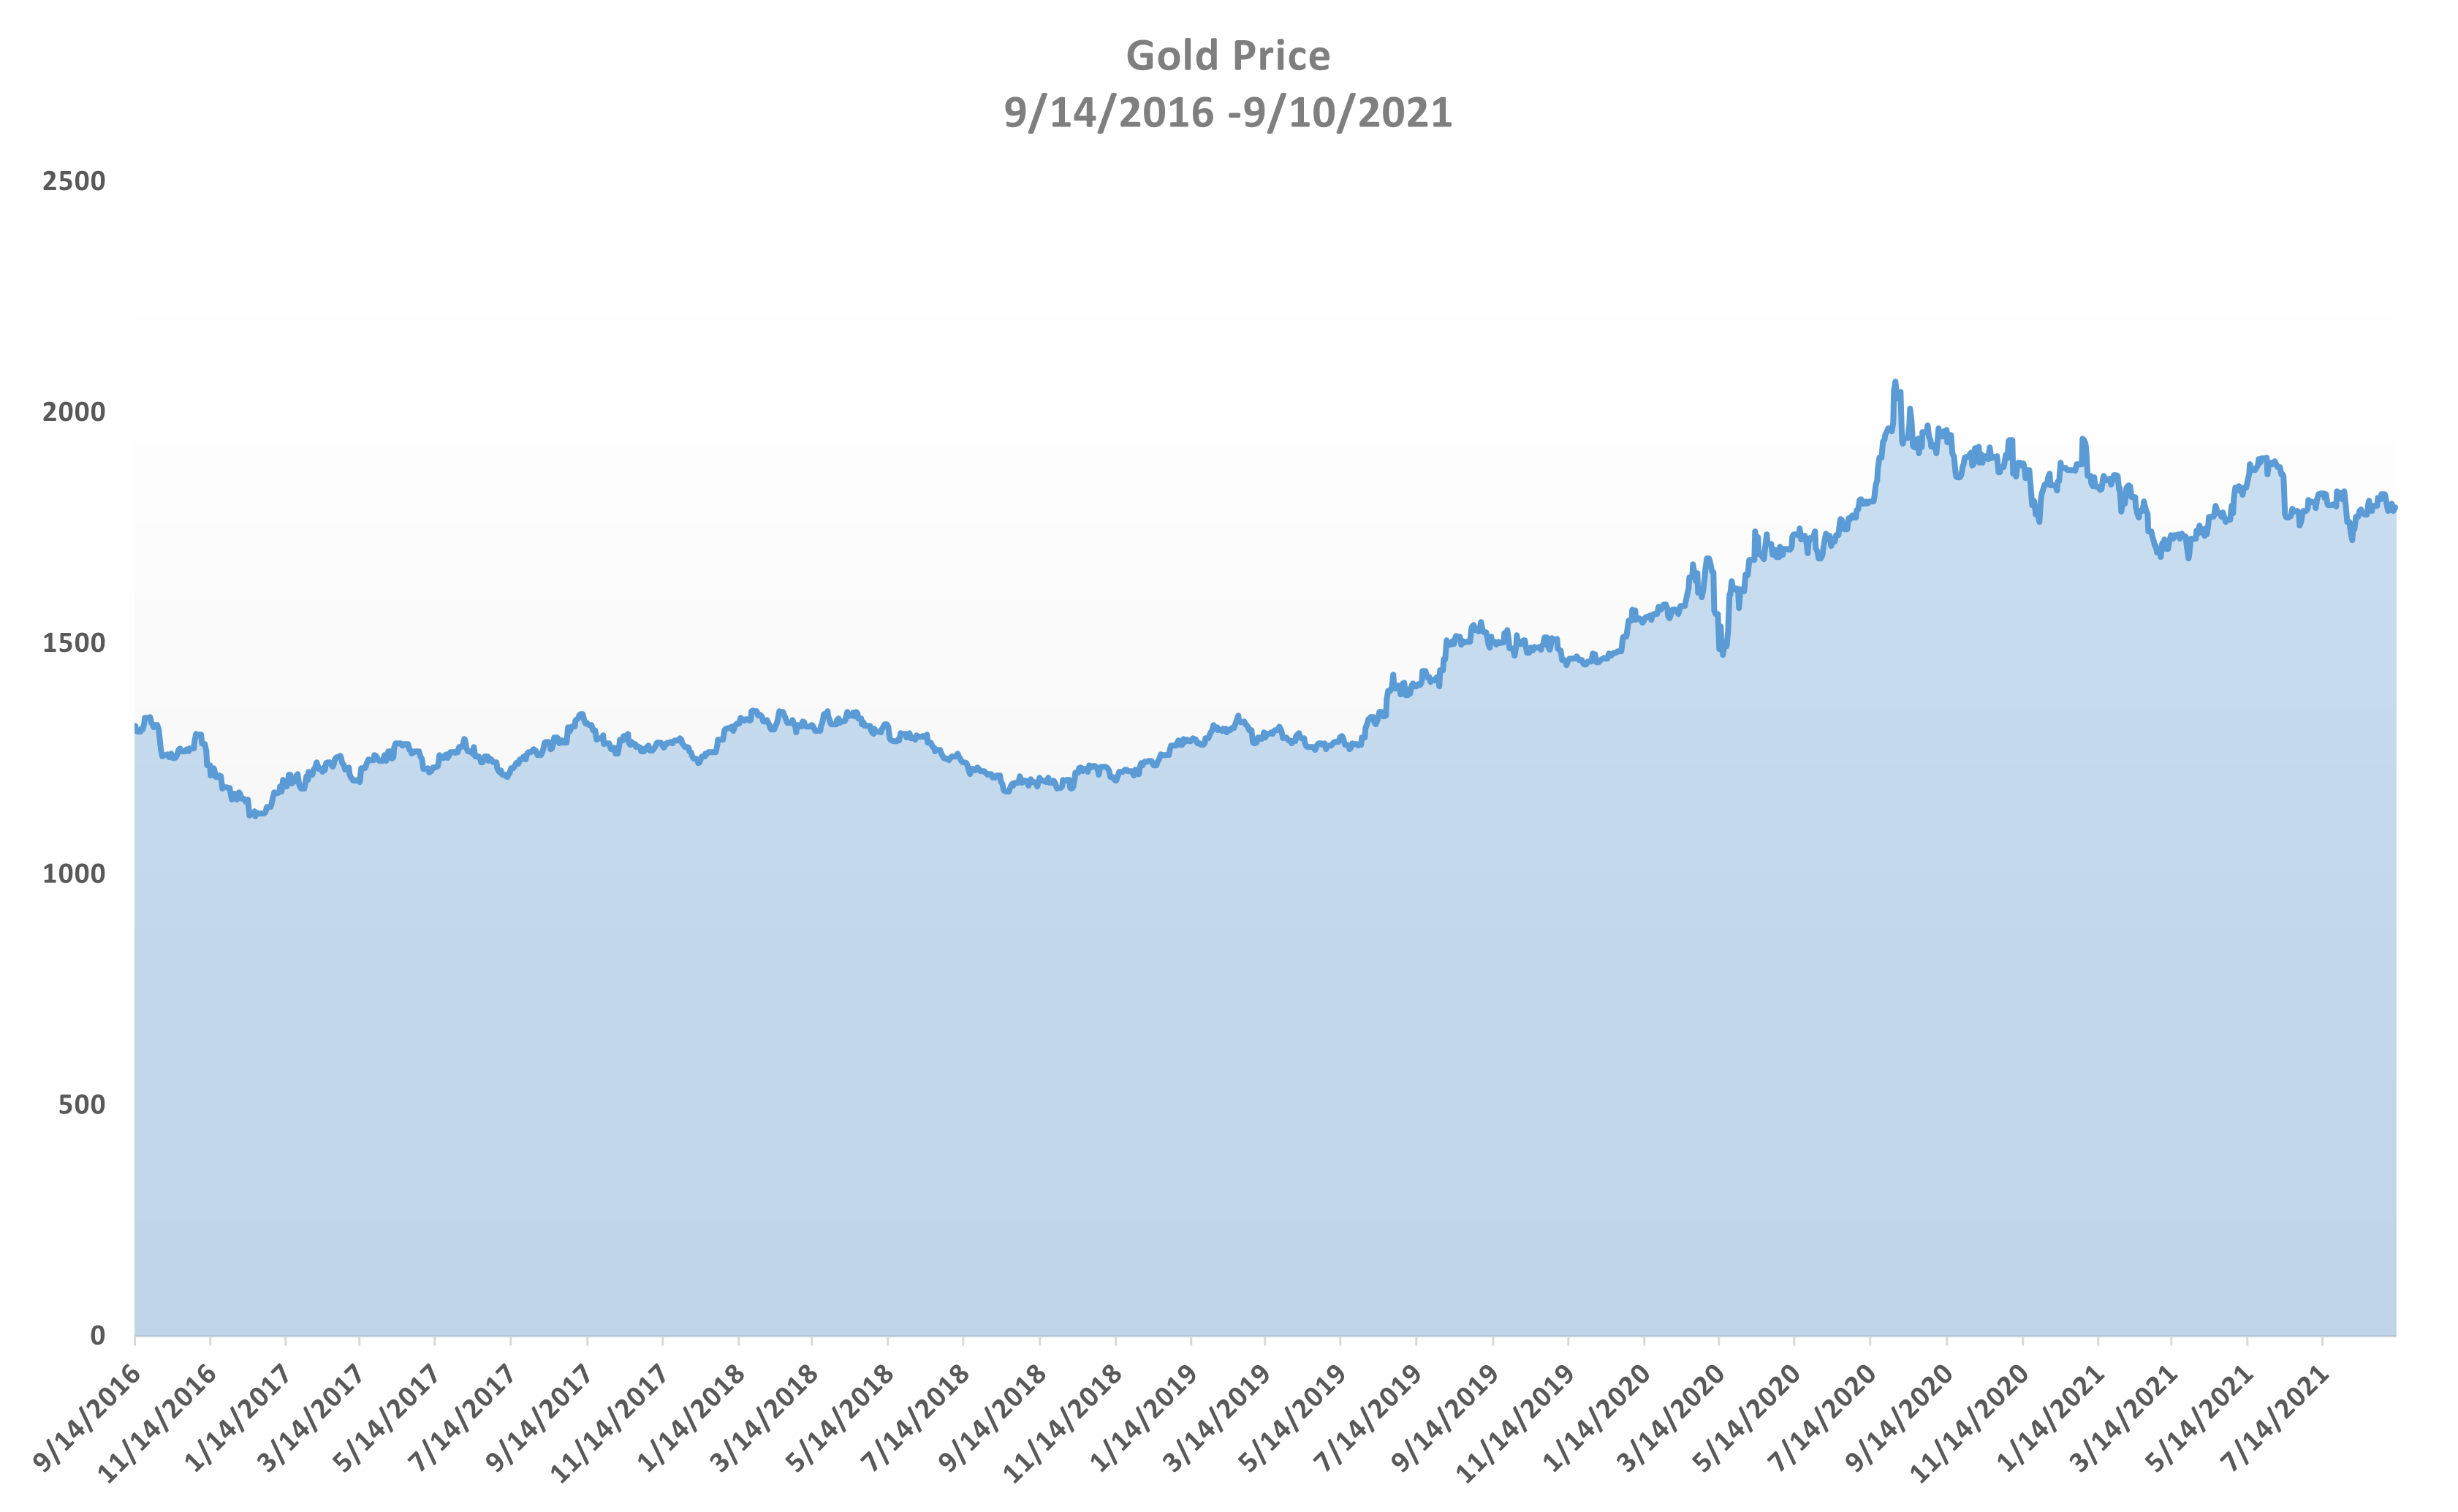
\includegraphics[[width=0.7\textwidth]{figures/fig1.png}
%     \caption{The name of figure} \label{fig:aa}
% \end{figure}
\begin{figure}[htp]
    \begin{subfigure}{.5\textwidth}
        \centering
        % include first image
        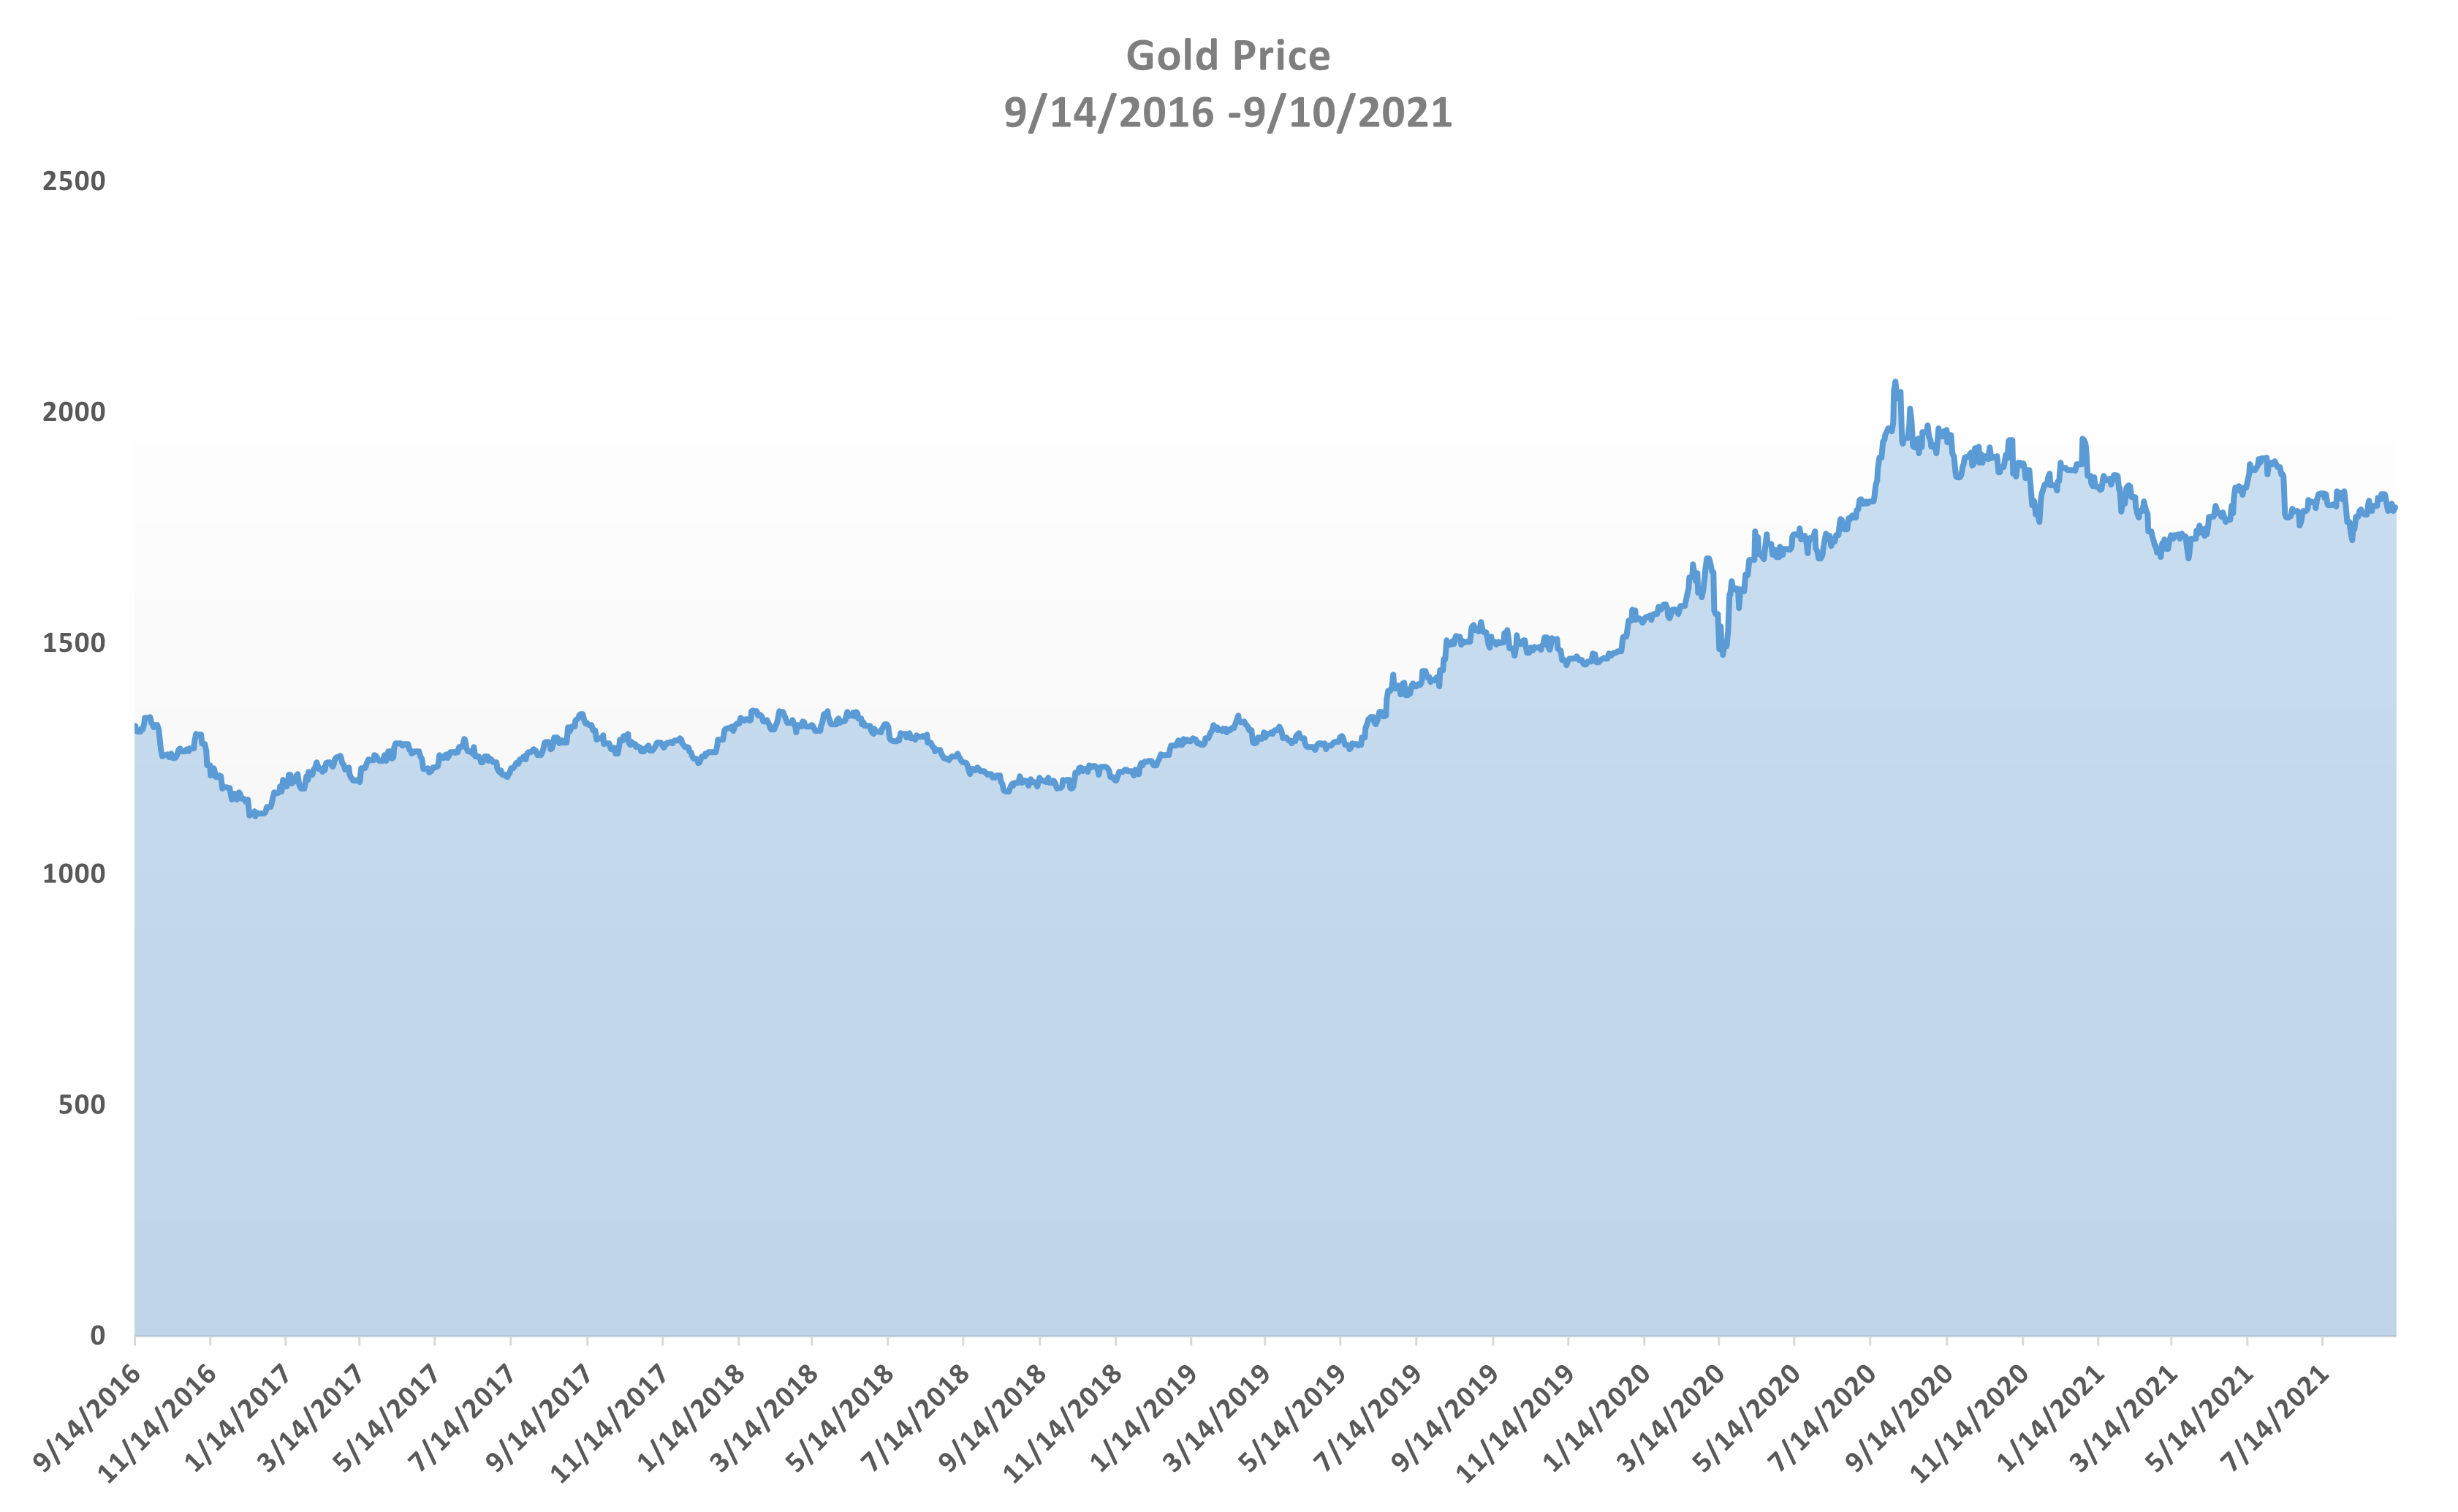
\includegraphics[width=.9\linewidth]{figures/fig1.png}  
        \caption{Gold Price}
        \label{fig1:1}
      \end{subfigure}
      \begin{subfigure}{.5\textwidth}
        \centering
        % include second image
        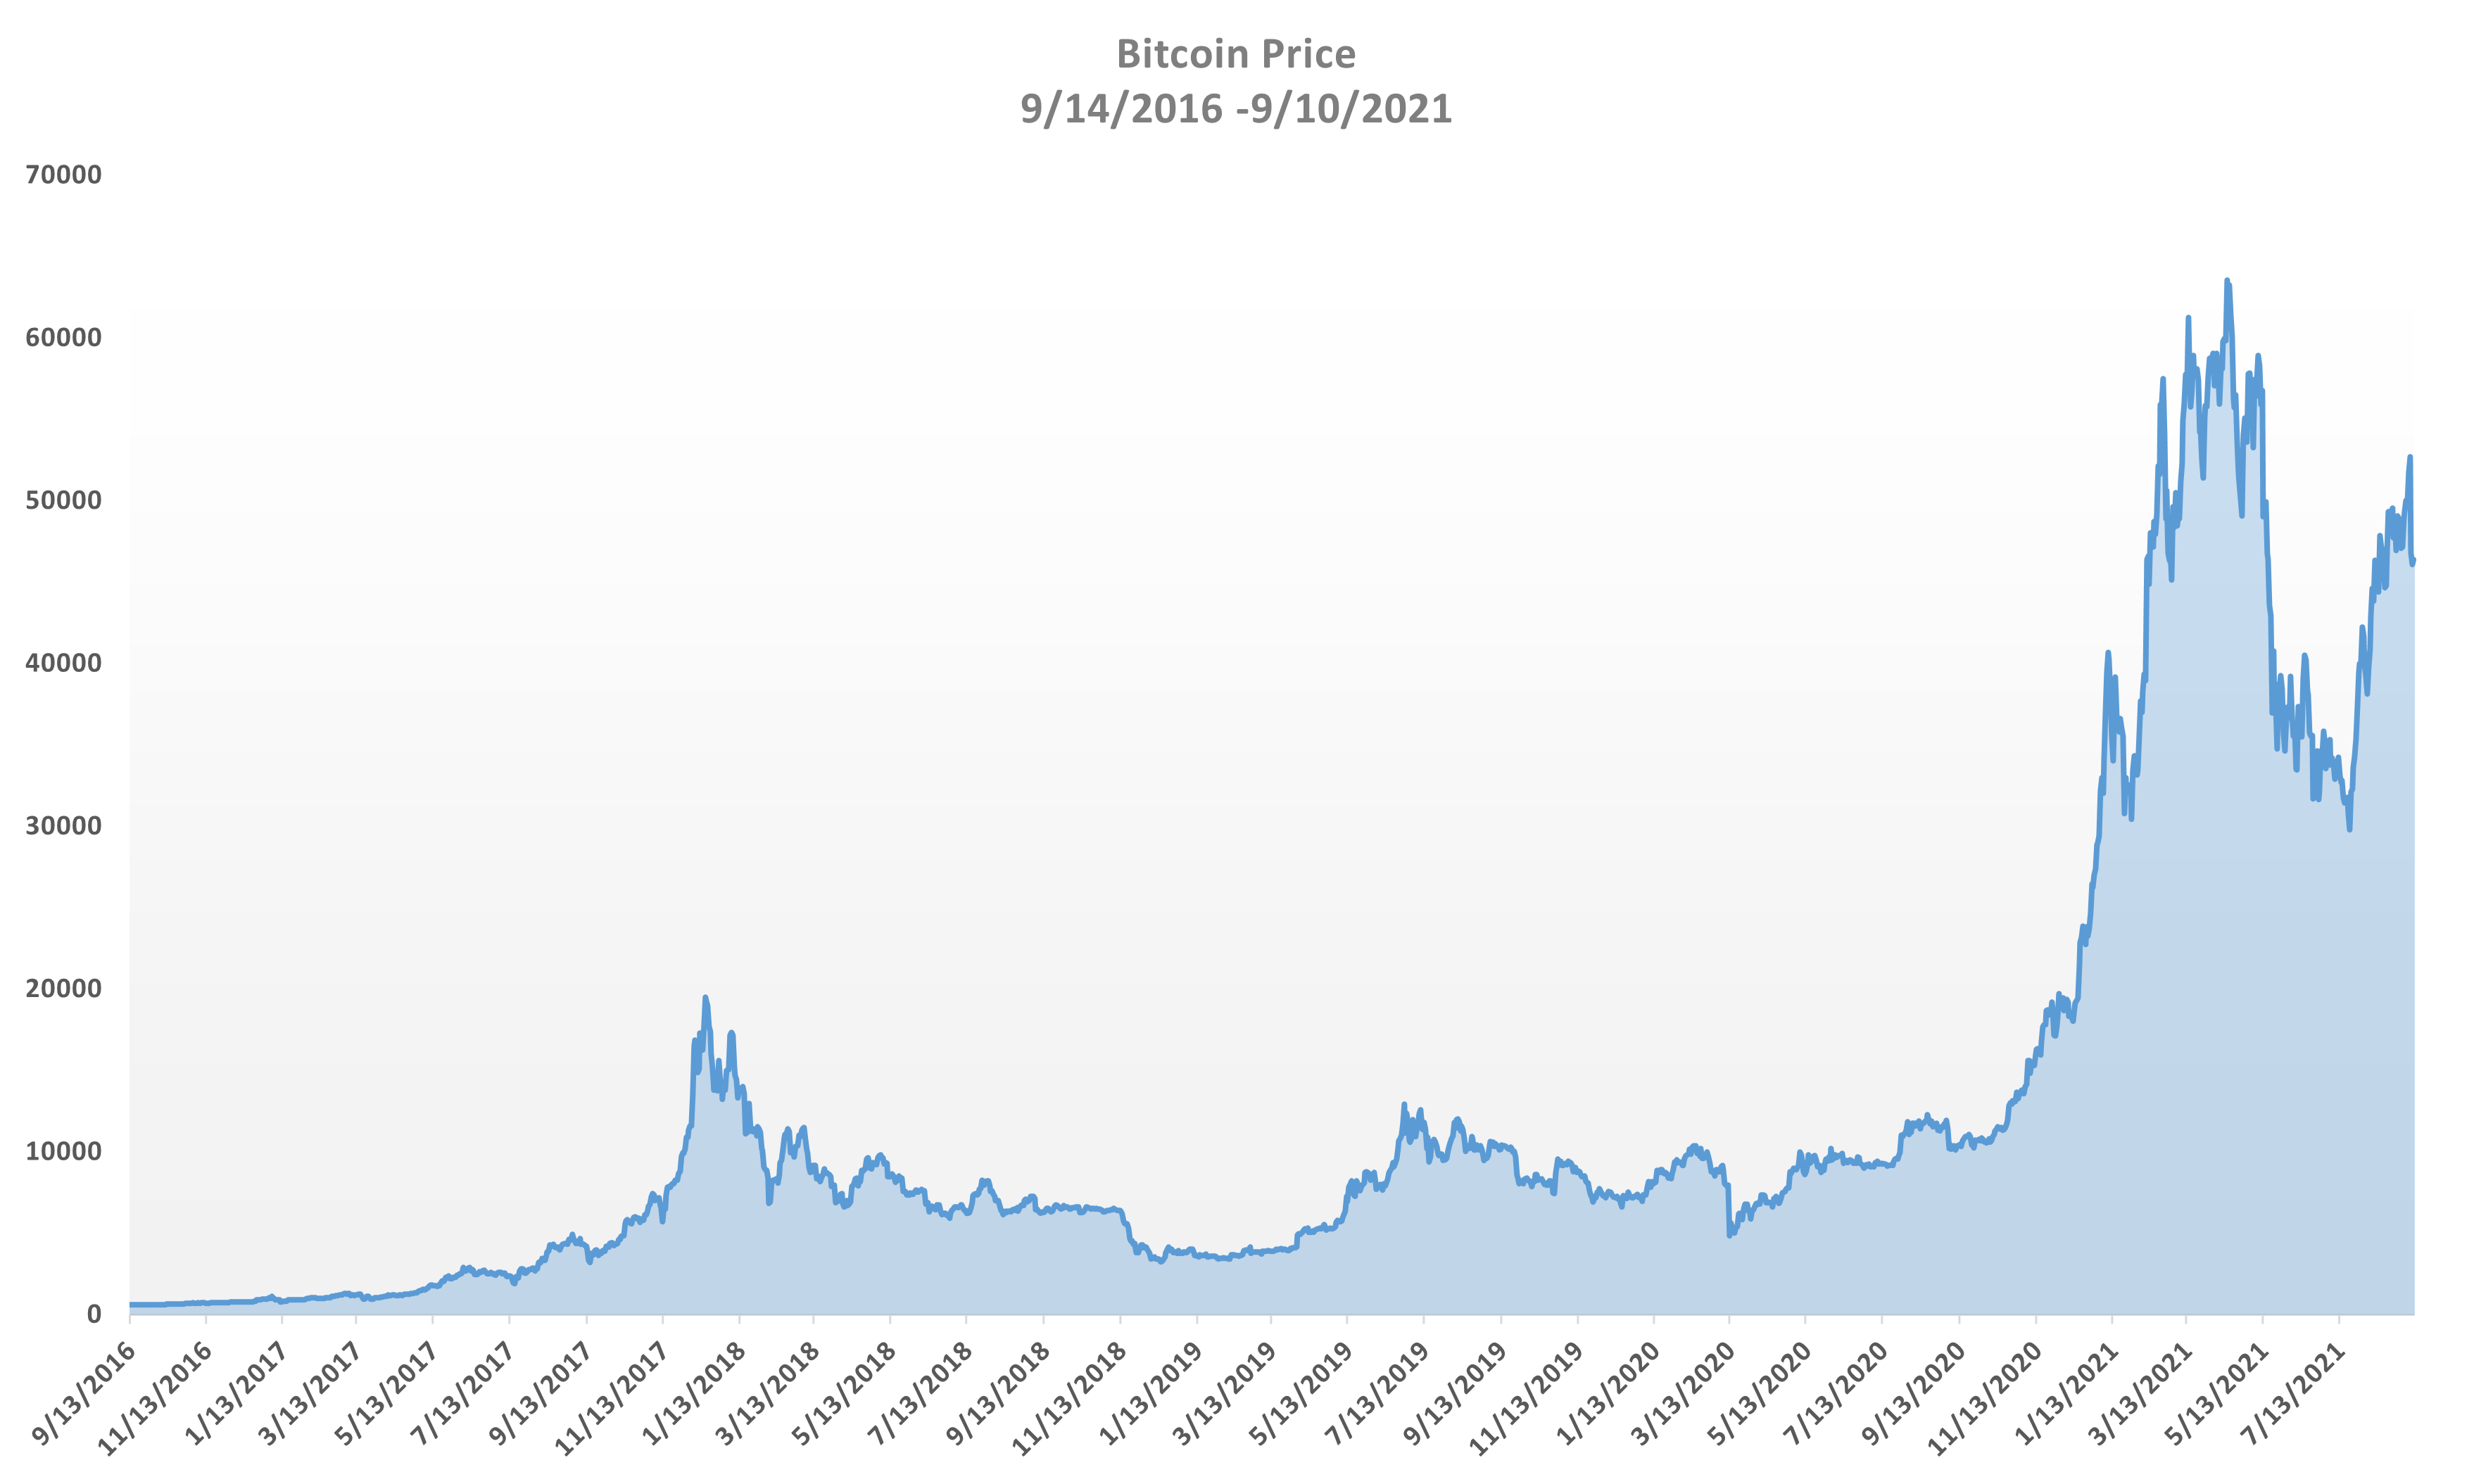
\includegraphics[width=.9\linewidth]{figures/fig2.png}  
        \caption{Bitcoin Price}
        \label{fig1:2}
      \end{subfigure}
      \caption{Price}
      \label{fig:fig1}
\end{figure}
\newpage
\subsection{Overview of Working Process}
Our team based on the following work map to solve this problem:
\begin{figure}[htp]
    \centering
        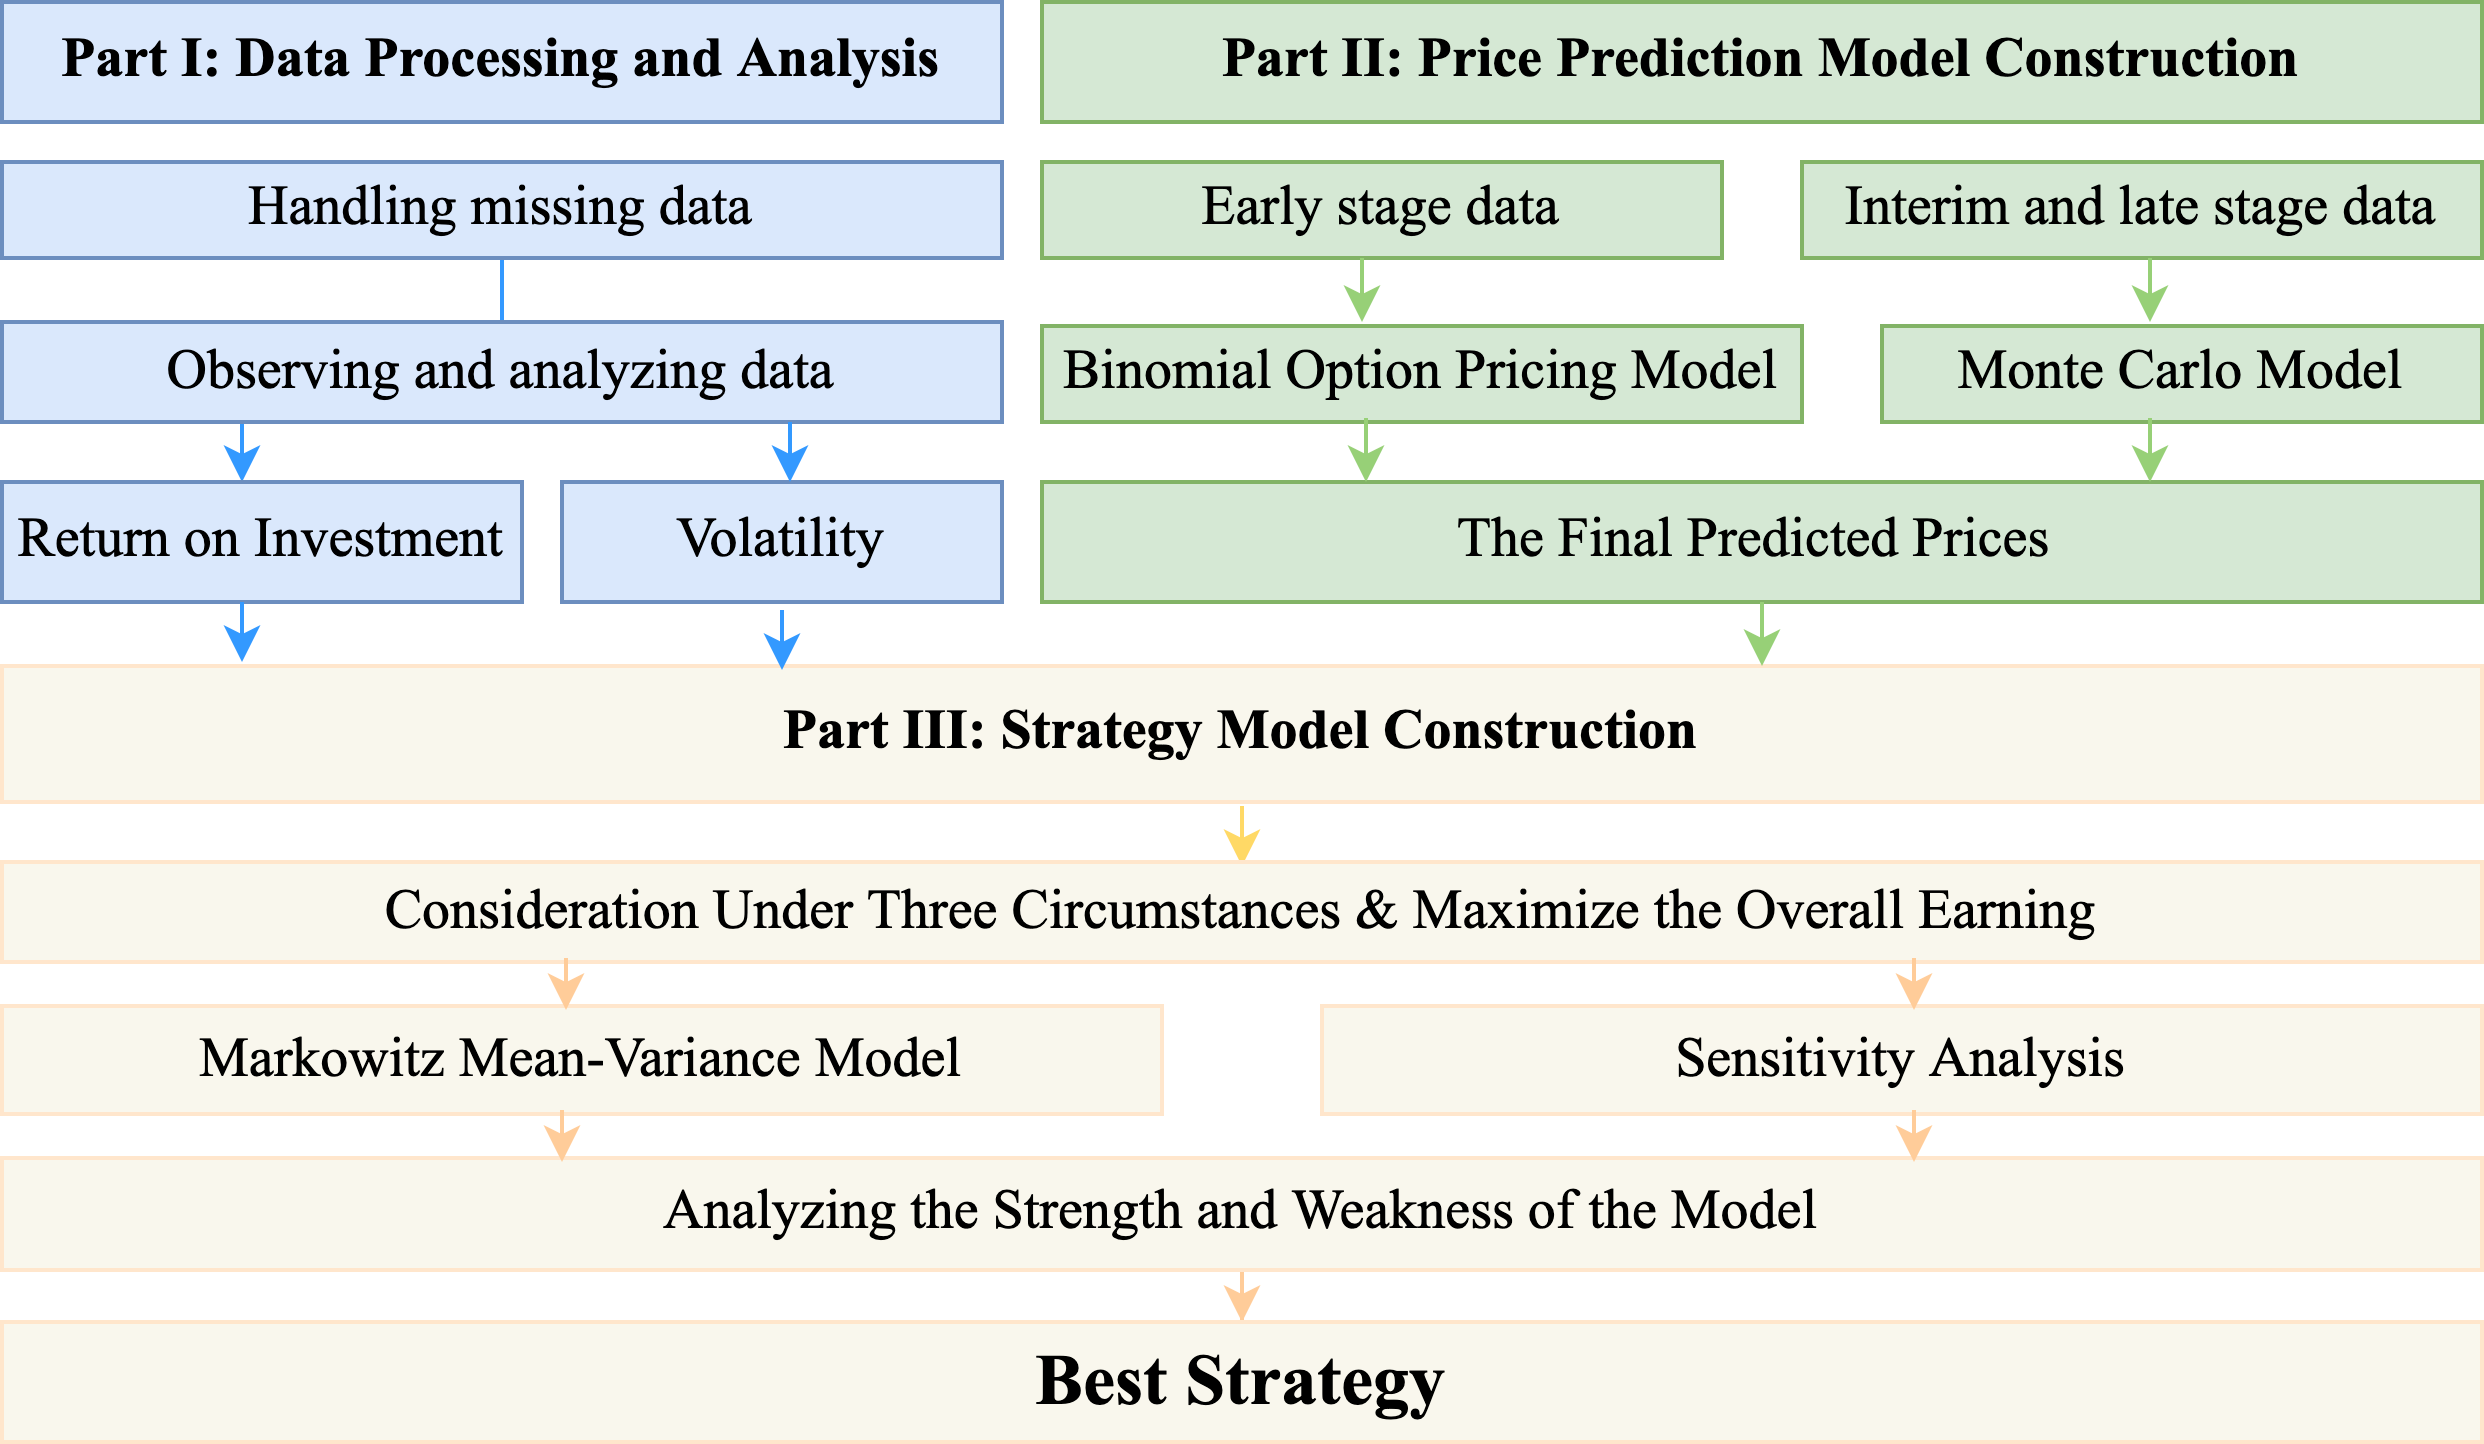
\includegraphics[width=.8\linewidth]{figures/process.png}  
        \caption{Working Process}
        \label{fig:fig2}
\end{figure}
\paragraph{}
In part I, we did simple processing to the prices of gold and bitcoin, and then analyzed the return on investment, volatility, and standard deviation of daily volatility.
\paragraph{}
In part II, we built the price prediction models to predict the next day's price. 
\begin{itemize}
    \item We used the Binomial Option Pricing model to predict the prices of gold and bitcoin for the first 500 days
    \item When the quantity of predicted prices of gold and bitcoin reaches 500, we change the binomial option pricing model into Monte Carlo method. 
\end{itemize}
Thus, we get a complete set of predicted prices for the entire five years.
\paragraph{}
In part III, by applying the Markowitz model to optimize our portfolio, we choose the strategy with the lowest risk rate under certain return conditions as the final result.
Finally, we used the above models to analyze the data that we obtained to get the sensitivity of the model. Based on the sensitivity, we give some suggestions for this solution to the trader. 
\section{Analysis of Data Sets }
\subsection{Handling Missing Values}
Gold trading is determined by the opening and closing of the market. From Figure 3, we can see that some data are missing.  To handle this issue, our team decided to use the latest trading day's gold price as the predicted gold price for that closing day, thus making the data continuous.
\begin{figure}[htp]
    \centering
        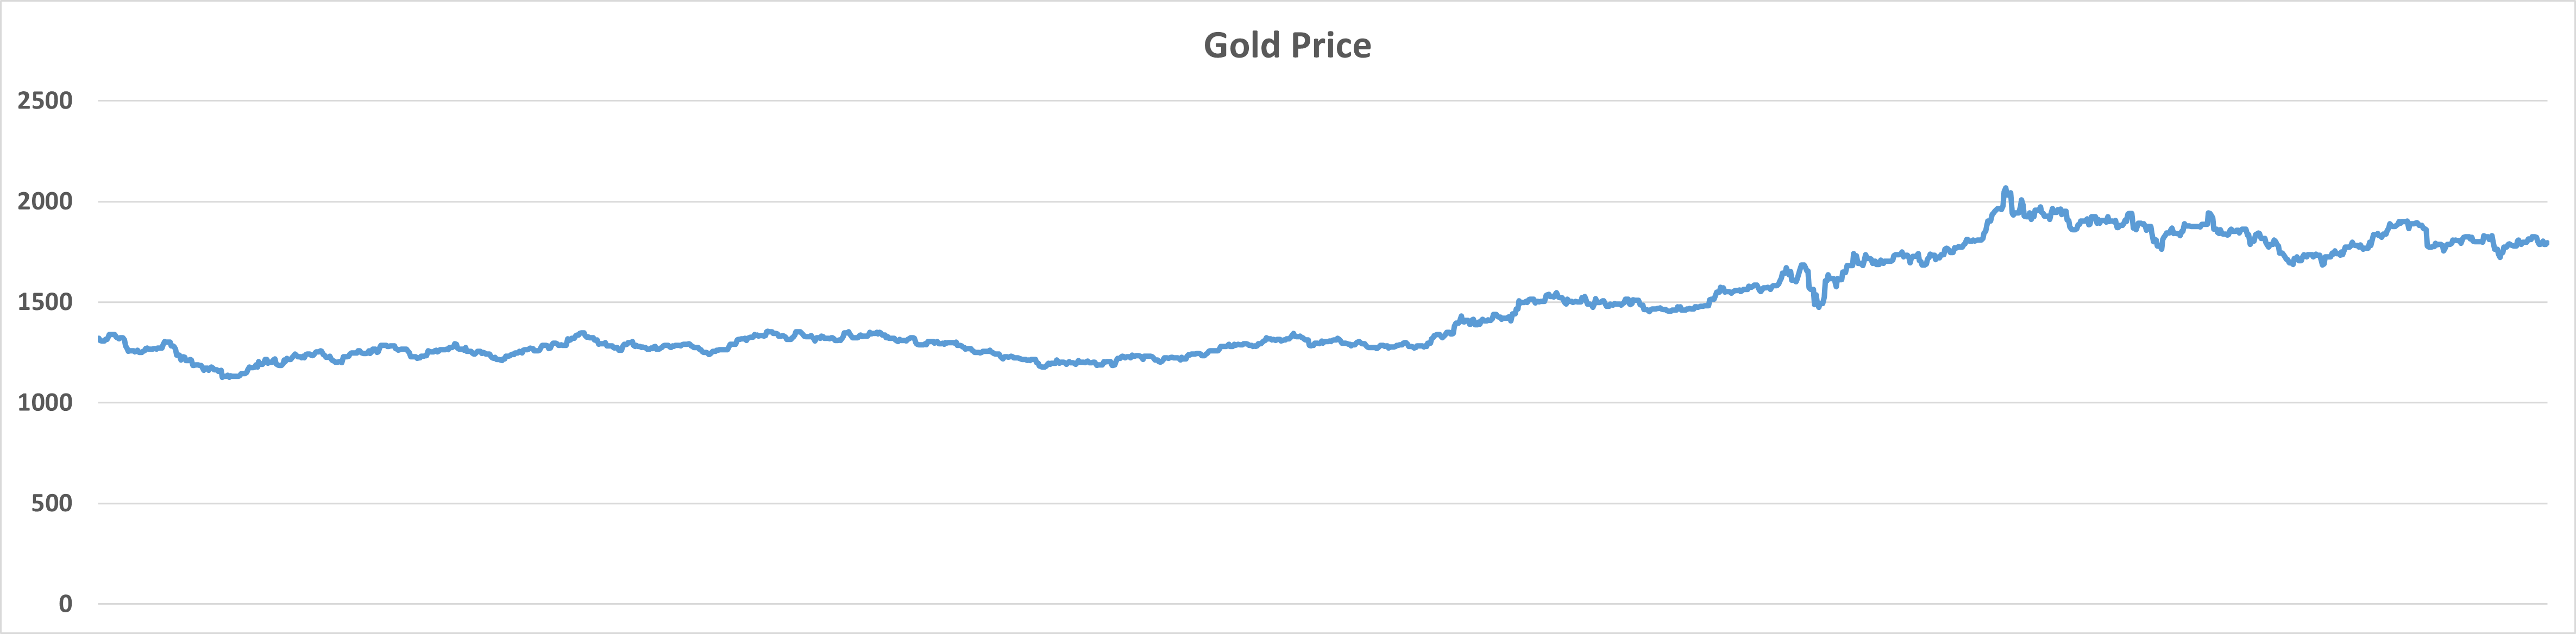
\includegraphics[width=.8\linewidth]{figures/gold_price_value.png}  
        \caption{Gold Price After Data Filling}
        \label{fig:gold_price}
\end{figure}
% \newpage
\subsection{Volatility of Gold and Bitcoin}

    \paragraph{}
    Volatility is the degree of fluctuation of the price in a financial asset and can reflect the level of risk of a financial asset. The higher the volatility, the greater the uncertainty of the asset's return. For this reason, volatility can define the riskiness of gold and BTC investments.The daily volatility is defined by

    \begin{equation}
        \nu_i=(\frac{p_i}{p'_i}-1)\times 100\%
    \end{equation}
    Because of instability of daily volatility, we decide the standard deviation (stdev) to determine the fluctuation of gold and BTC prices. 
    The standard deviation of daily volatility is defined by 
 
    \begin{equation}
        \sigma_i=\sqrt{\frac{(p_i-\overline{p})^2}{n-1}}.
    \end{equation}
    where $\overline{p}$ is the expected value of the known historical data, \emph{i.e.}, all data from $9/11/2016$ to the $(i-1)$-th day.
    \paragraph{}
    Return on investment (ROI) is defined by
    \begin{equation}
        \mu_i=\frac{\rho_i-\Omega_i-(\Omega_i+\rho_i)\times \alpha_i}{\Omega_i}\times 100\%.
    \end{equation}
    The ROI $\mu_i$ clearly shows that trading in a certain time period is the most profitable at that time. 
    \begin{table}
        \begin{center}
        \begin{tabular}{p{80pt}p{280pt}}
        \toprule
        Symbol       & Definitions \\
        \midrule
        $\nu_i$       &  Daily volatility of $i$-th day. \\
        % \midrule
        $\sigma_i$    & Standard deviation of daily volatility before $i$-th day. \\
        $p_i$     & The price of $i$-th day. \\
        $p'_i$& The price of $i-1$-th day,\emph{i.e.} $p_i$. \\
        $\alpha_{G},\alpha_{B}$& Commission fee rate per transaction of gold and Bitcoin.\\
        $\mu_i$&Return on investment(ROI) of $i$-th day.\\
        $\Omega_i$ & Initial investment cost of $i$-th day.\\
        $\rho_i$&Recovery of investment quantity of $i$-th day.\\
        \bottomrule 
        \end{tabular}
        \end{center}
        \end{table}
    % \begin{figure}[htp]
    %     \centering
    %         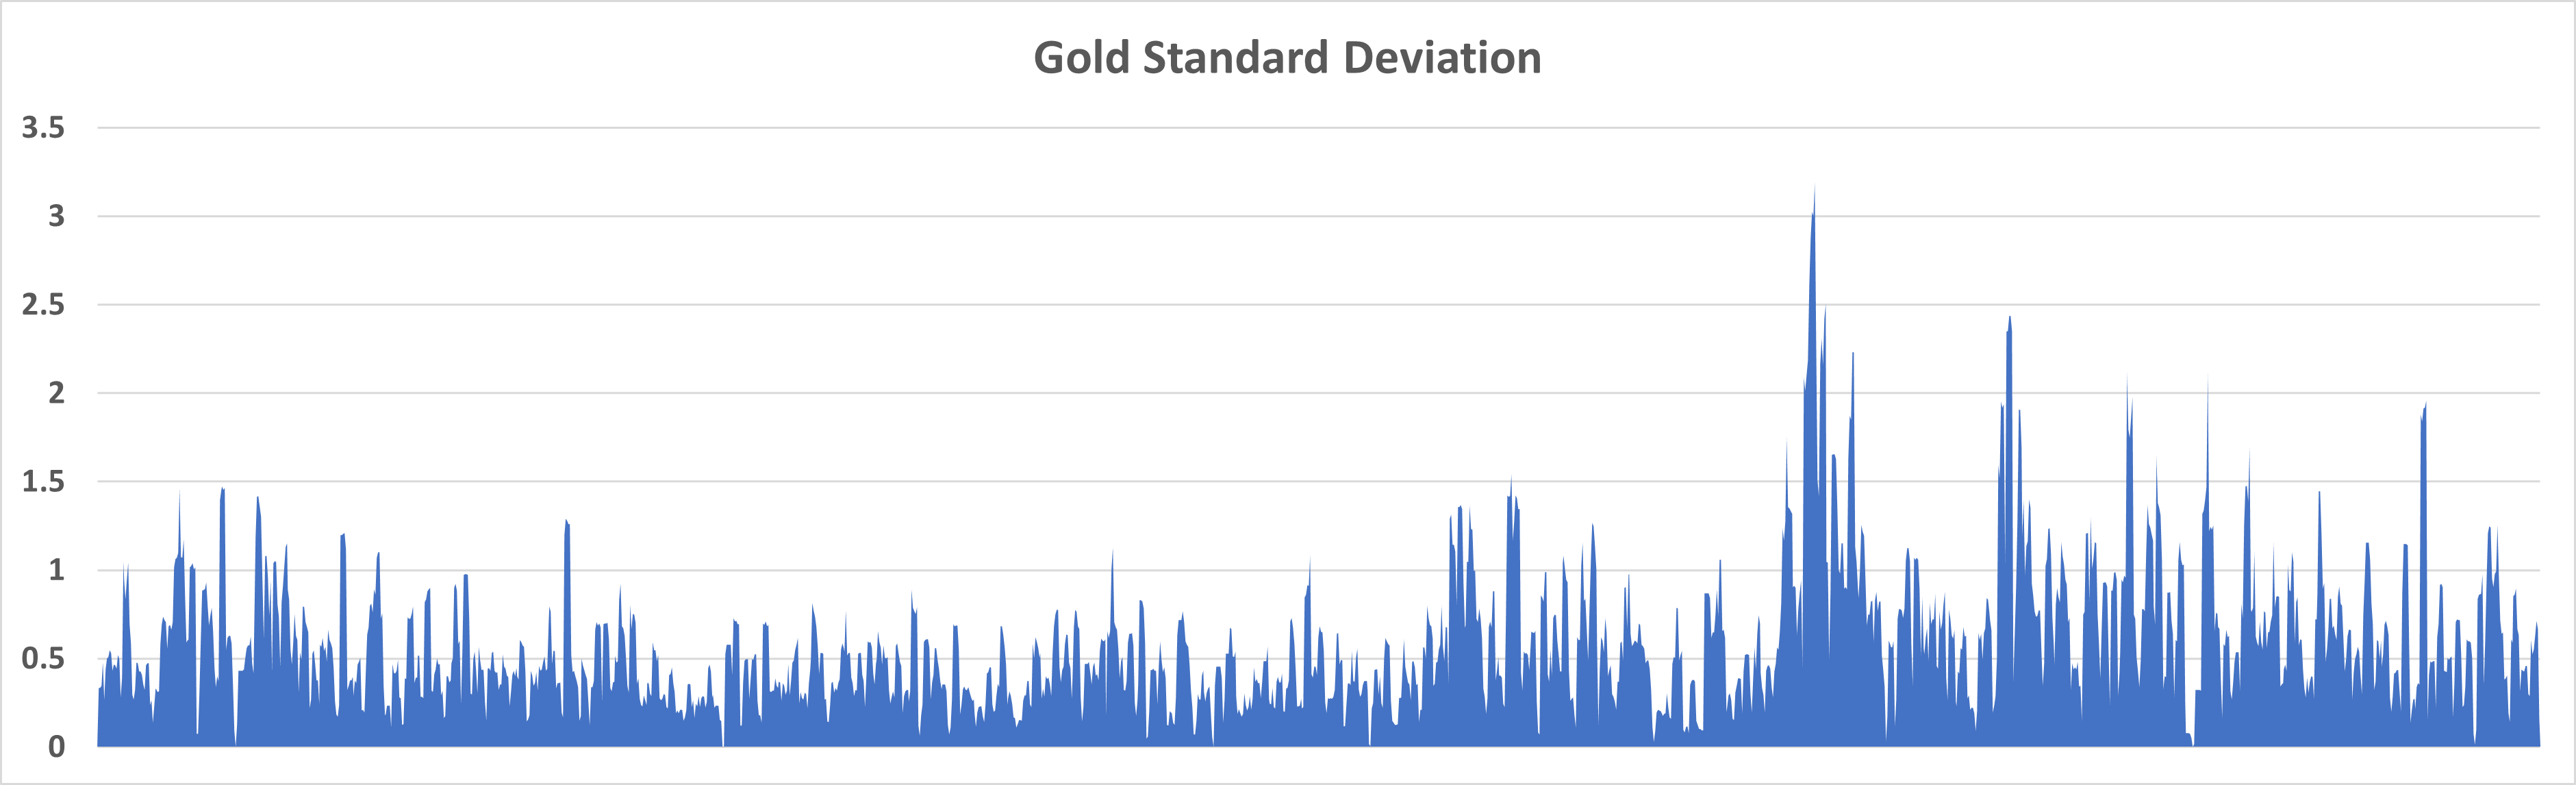
\includegraphics[width=.8\linewidth]{figures/gold_std.png}  
    %         \caption{Gold Standard Deviation}
    %         \label{fig:gold_std}
    % \end{figure}
\section{Prediction Model Construction: Early Stage Data }
\subsection{Building The Binomial Option Pricing Model (BOPM)}
\paragraph{}
Since for the first few days, the quantity of data that we can use for predicting the price of the coming day is comparatively limited. Given this circumstance, we decide to use the Binomial Option Pricing Model to predict the price of gold and bitcoin for the first 500 days (9/11/2016 to 1/23/18)
\begin{figure}[htp]
    \centering
        
\includegraphics[width=.4\linewidth]{figures/fig3.png}  
        \caption{The Binomial Option Pricing Model}
        \label{fig:fig3}
\end{figure}
\paragraph{}
Although Binomial Option Pricing Model can actually predict prices for many days in the future, we noticed that every time when we predict the price for the next day, we will have an updated data set consisting of all the prices up to date. So instead of predicting many day's prices at one time, our team decided to only predict the next day's price each time using the latest up-to-date data to reach higher accuracy.  The predict price of $i$-th day $p'_{i}$ can be calculated with
\begin{equation}
    p'_{i}=e^{\sigma'_i\sqrt{\frac{t}{i-1}}} \frac{e^{\frac{rt}{i-1}}-e^{-\sigma'_i\sqrt{\frac{t}{i-1}}}}{e^{\sigma'_i\sqrt{\frac{t}{i-1}}}-e^{-\sigma'_i\sqrt{\frac{t}{i-1}}}} p_{i-1}+e^{-\sigma'_i\sqrt{\frac{t}{i-1}}} (1-\frac{e^{\frac{rt}{i-1}}-e^{-\sigma'_i\sqrt{\frac{t}{i-1}}}}{e^{\sigma'_i\sqrt{\frac{t}{i-1}}}-e^{-\sigma'_i\sqrt{\frac{t}{i-1}}}})p_{i-1}
\end{equation}
where $\sigma'_i$ is the standard deviation of daily price before $i$-th day, $t$ is the number of period of one day. In our model, $t=1$
\subsection{Predicting Short-Term Data (first 500 days)}
\subsubsection{Price Prediction for Gold}
For gold, 9/11/2016 is not a trading day, the first trading day is 9/12/2016. Since on this day, we only have one price data, denoted as $P_1$, which is far from enough to predict the next day's price. Therefore, to be on the safe side, our team decided to assume that the 9/13/2016 predicted price, denoted as $P'_2$, is a random number fluctuating within the range of $(P_1\times95\%, P_1\times105\%)$, thus making the trading strategy for 9/12/2016. 
\paragraph{}
When we come to the second trading day 9/12/2016, we already have two day's price data, $P_1$ and $P_2$, we can then use the Binomial Option Pricing model to do price prediction starting from this day.
Starting from the second trading day 9/13/2016, every time we predict the price for the next day, our prediction model will base on all the historical data up to that day and output two predicted prices, one is $p_{i-1}e^{\sigma'_i\sqrt{\frac{t}{i-1}}}$, with probability $\frac{e^{\frac{rt}{i-1}}-e^{-\sigma'_i\sqrt{\frac{t}{i-1}}}}{e^{\sigma'_i\sqrt{\frac{t}{i-1}}}-e^{-\sigma'_i\sqrt{\frac{t}{i-1}}}}$, the other one is $p_{i-1}e^{-\sigma'_i\sqrt{\frac{t}{i-1}}}$, with $1-\frac{e^{\frac{rt}{i-1}}-e^{-\sigma'_i\sqrt{\frac{t}{i-1}}}}{e^{\sigma'_i\sqrt{\frac{t}{i-1}}}-e^{-\sigma'_i\sqrt{\frac{t}{i-1}}}}$ probability. After that, the model would calculate the mathematical expectation of the two prices $p_{i-1}e^{\sigma'_i\sqrt{\frac{t}{i-1}}}$ and $p_{i-1}e^{-\sigma'_i\sqrt{\frac{t}{i-1}}}$, and take the expectation as predicted price for the next day. Figure \ref{fig4:2} is the result of our gold price prediction for the first 500 days and Figure \ref{fig5:2} its error rate.
\begin{figure}[htp]
    \centering
    % include second image
    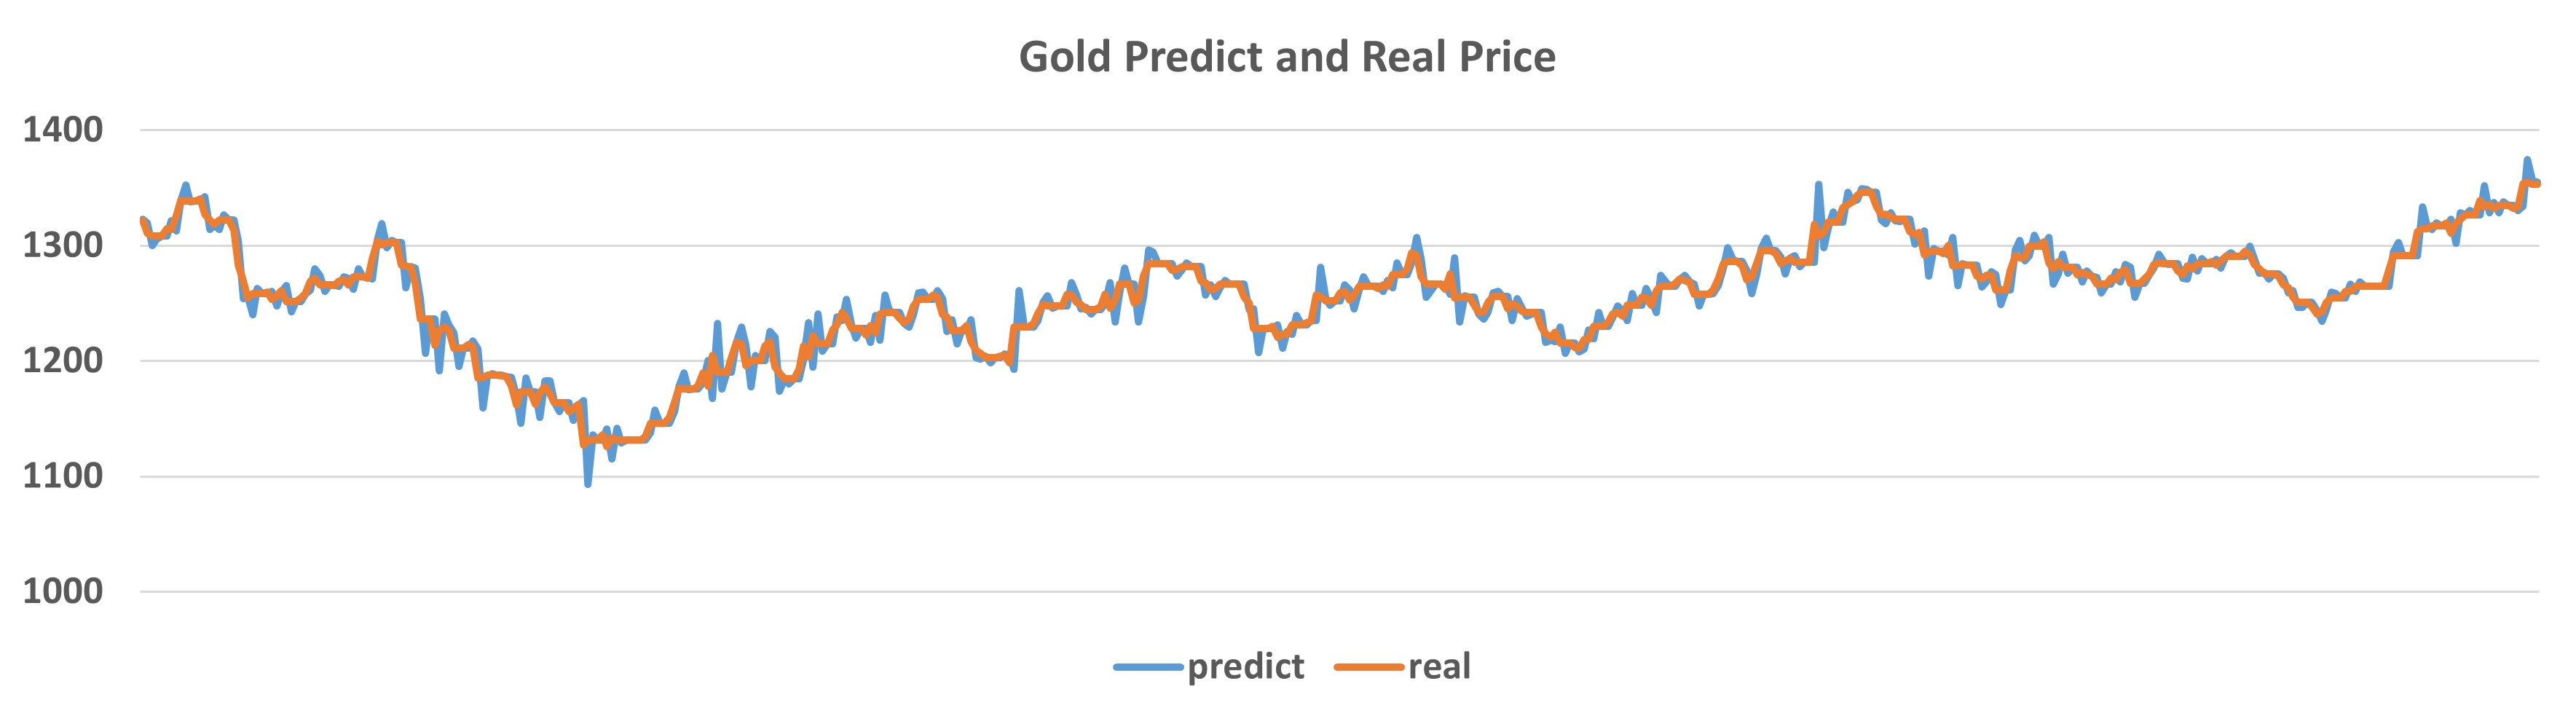
\includegraphics[width=.8\linewidth]{figures/fig5}  
    \caption{Gold Prediction Price}
    \label{fig4:2}
\end{figure}

\begin{figure}[htp]
    \centering
    % include second image
    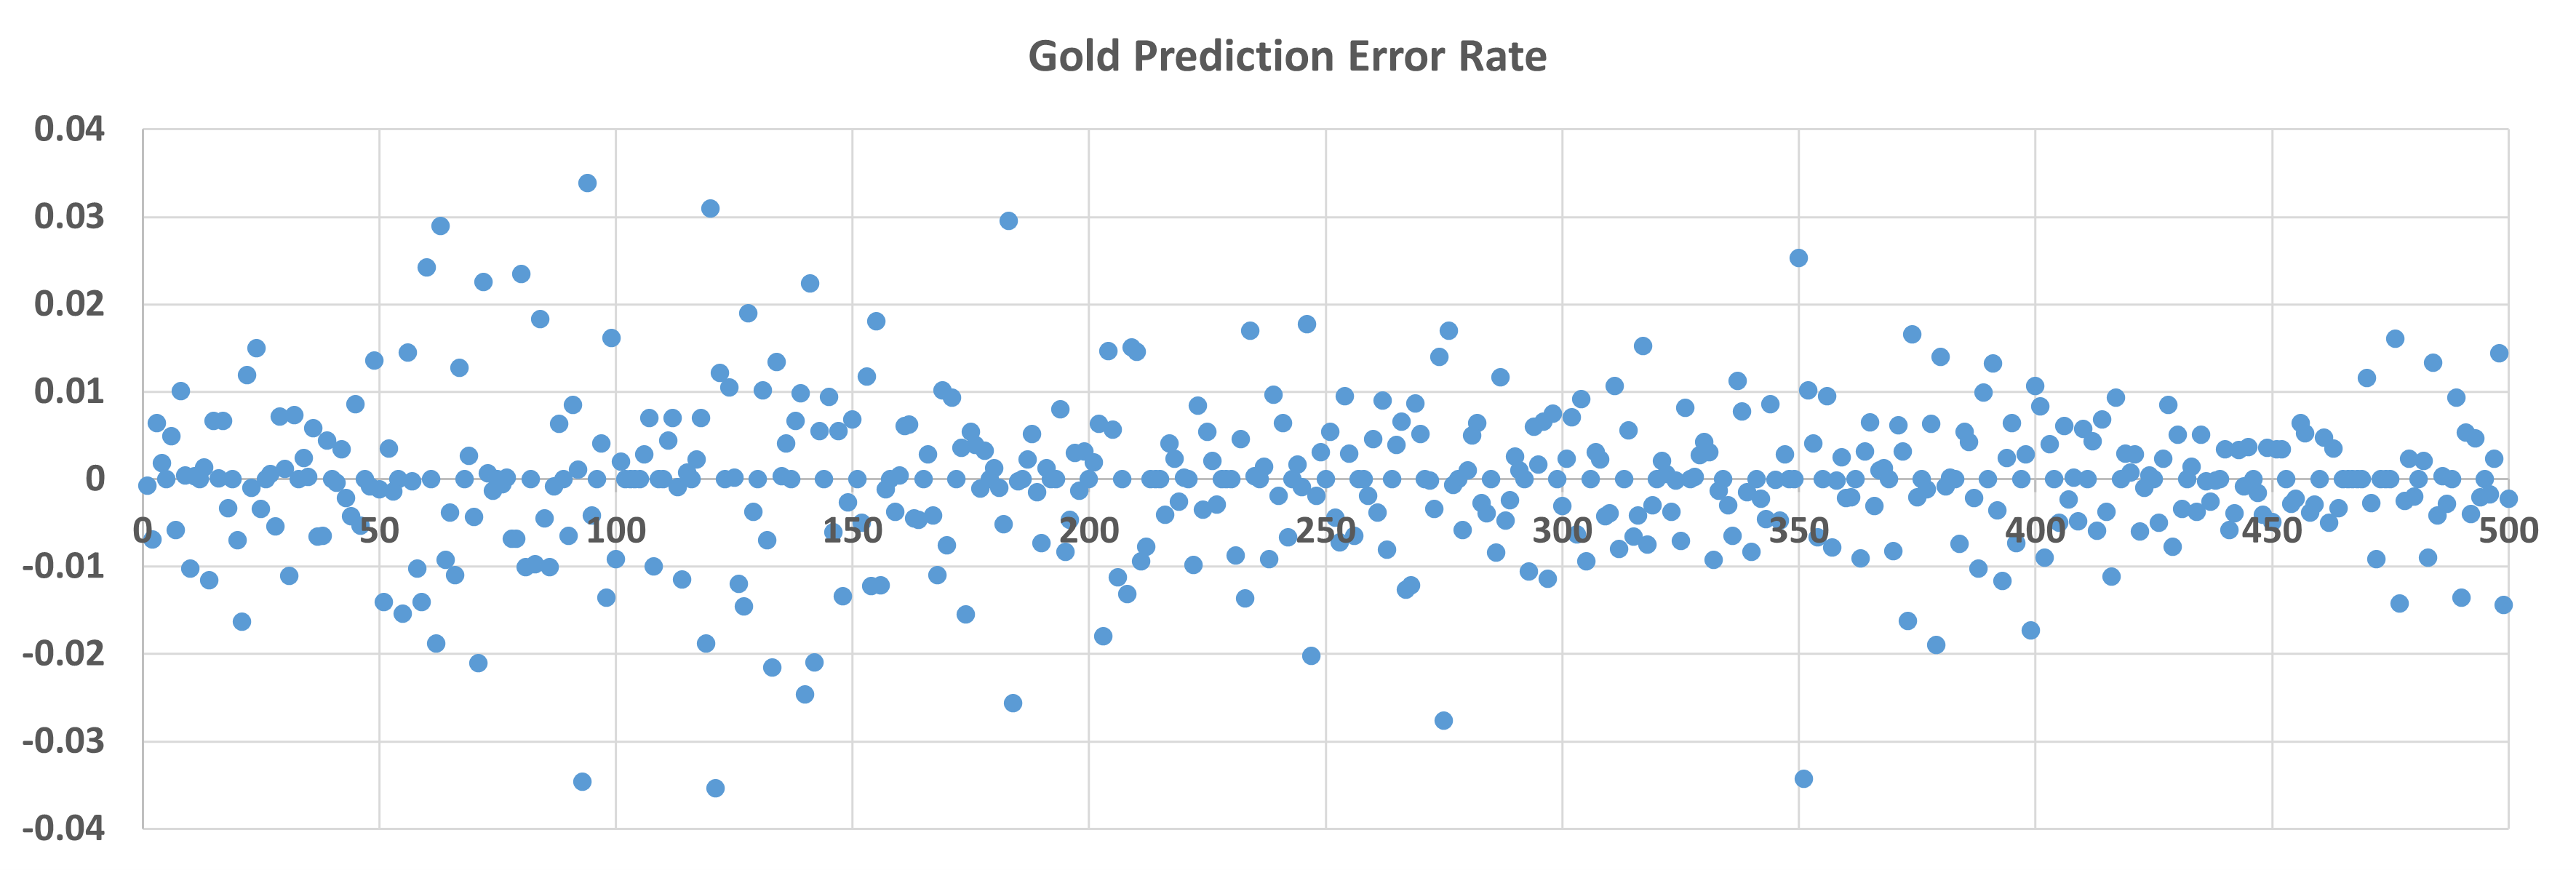
\includegraphics[width=0.8\linewidth]{figures/fig6}  
    \caption{Gold Prediction Error Rate}
    \label{fig5:2}
\end{figure}

% \newpage
\subsubsection{Price Prediction for Bitcoin}
\paragraph{}
For Bitcoin, 9/11/2016 is the first trading day. Since on this day, we only have one price data, denoted as $P_1$, which is far from enough to predict the next day's price. Therefore, to be on the safe side, our team decided to assume that the 9/12/2016 predicted price, denoted as $P'_2$, is a random number fluctuating within the range of $(P_1\times95\%, P_1\times105\%)$, thus making the trading strategy for 9/11/2016.
\paragraph{}
When we come to the second trading day 9/12/2016, we already have two day's price data, $P_1$ and $P_2$, we can then use the Binomial Option Pricing model to do price prediction starting from this day.Figure \ref{fig4:1} is the result of our gold price prediction for the first 500 days and Figure \ref{fig5:1} its error rate.
\begin{figure}[htp]
    \centering
        % include first image
    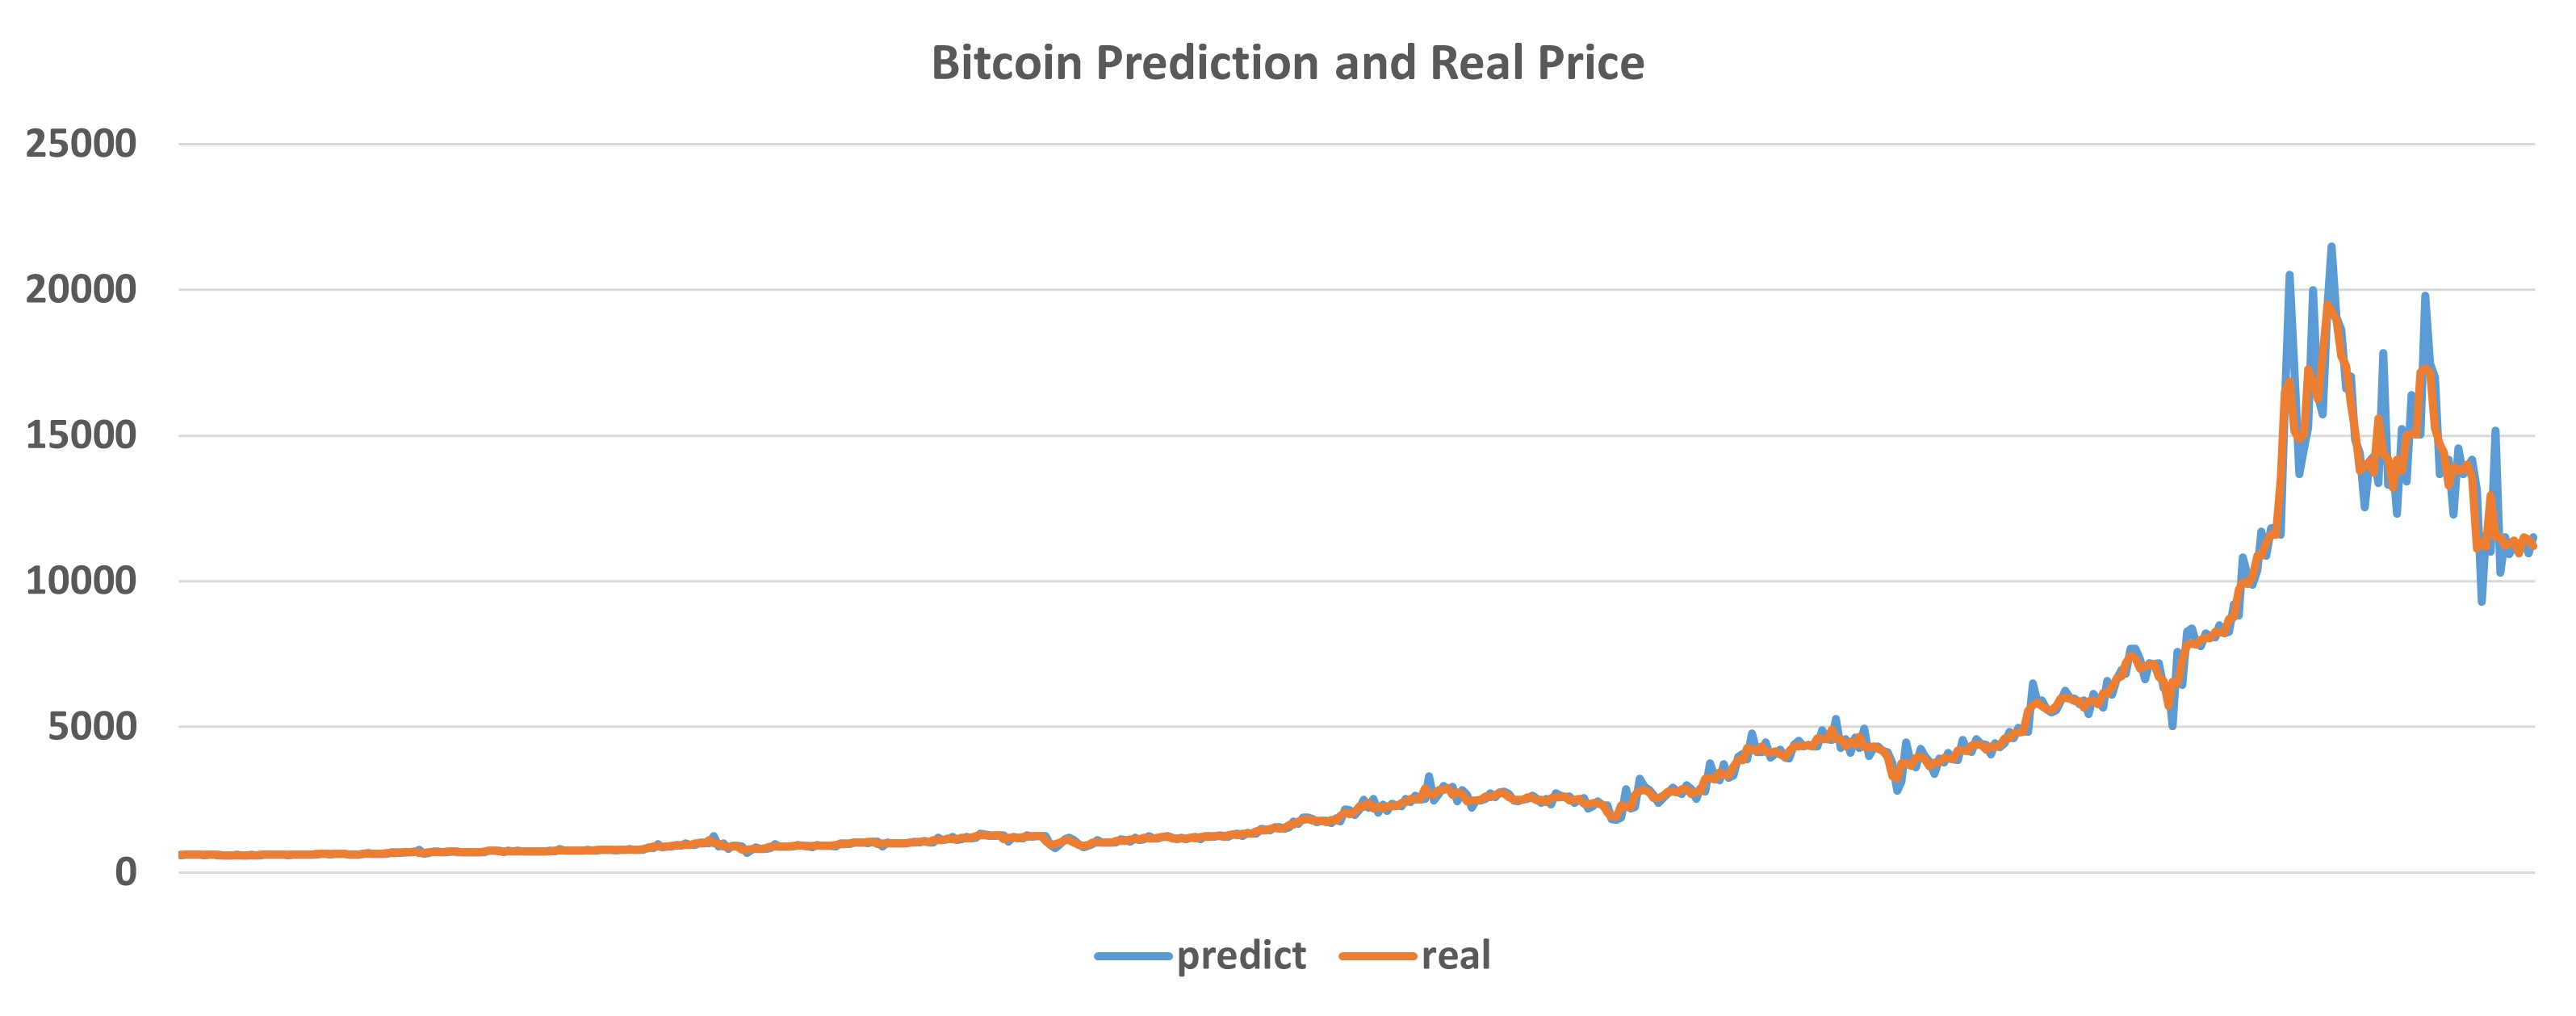
\includegraphics[width=.8\linewidth]{figures/fig4.jpg}  
    \caption{Bitcoin Prediction Price}
    \label{fig4:1}
\end{figure}
\begin{figure}[htp]
    \centering
    % include first image
    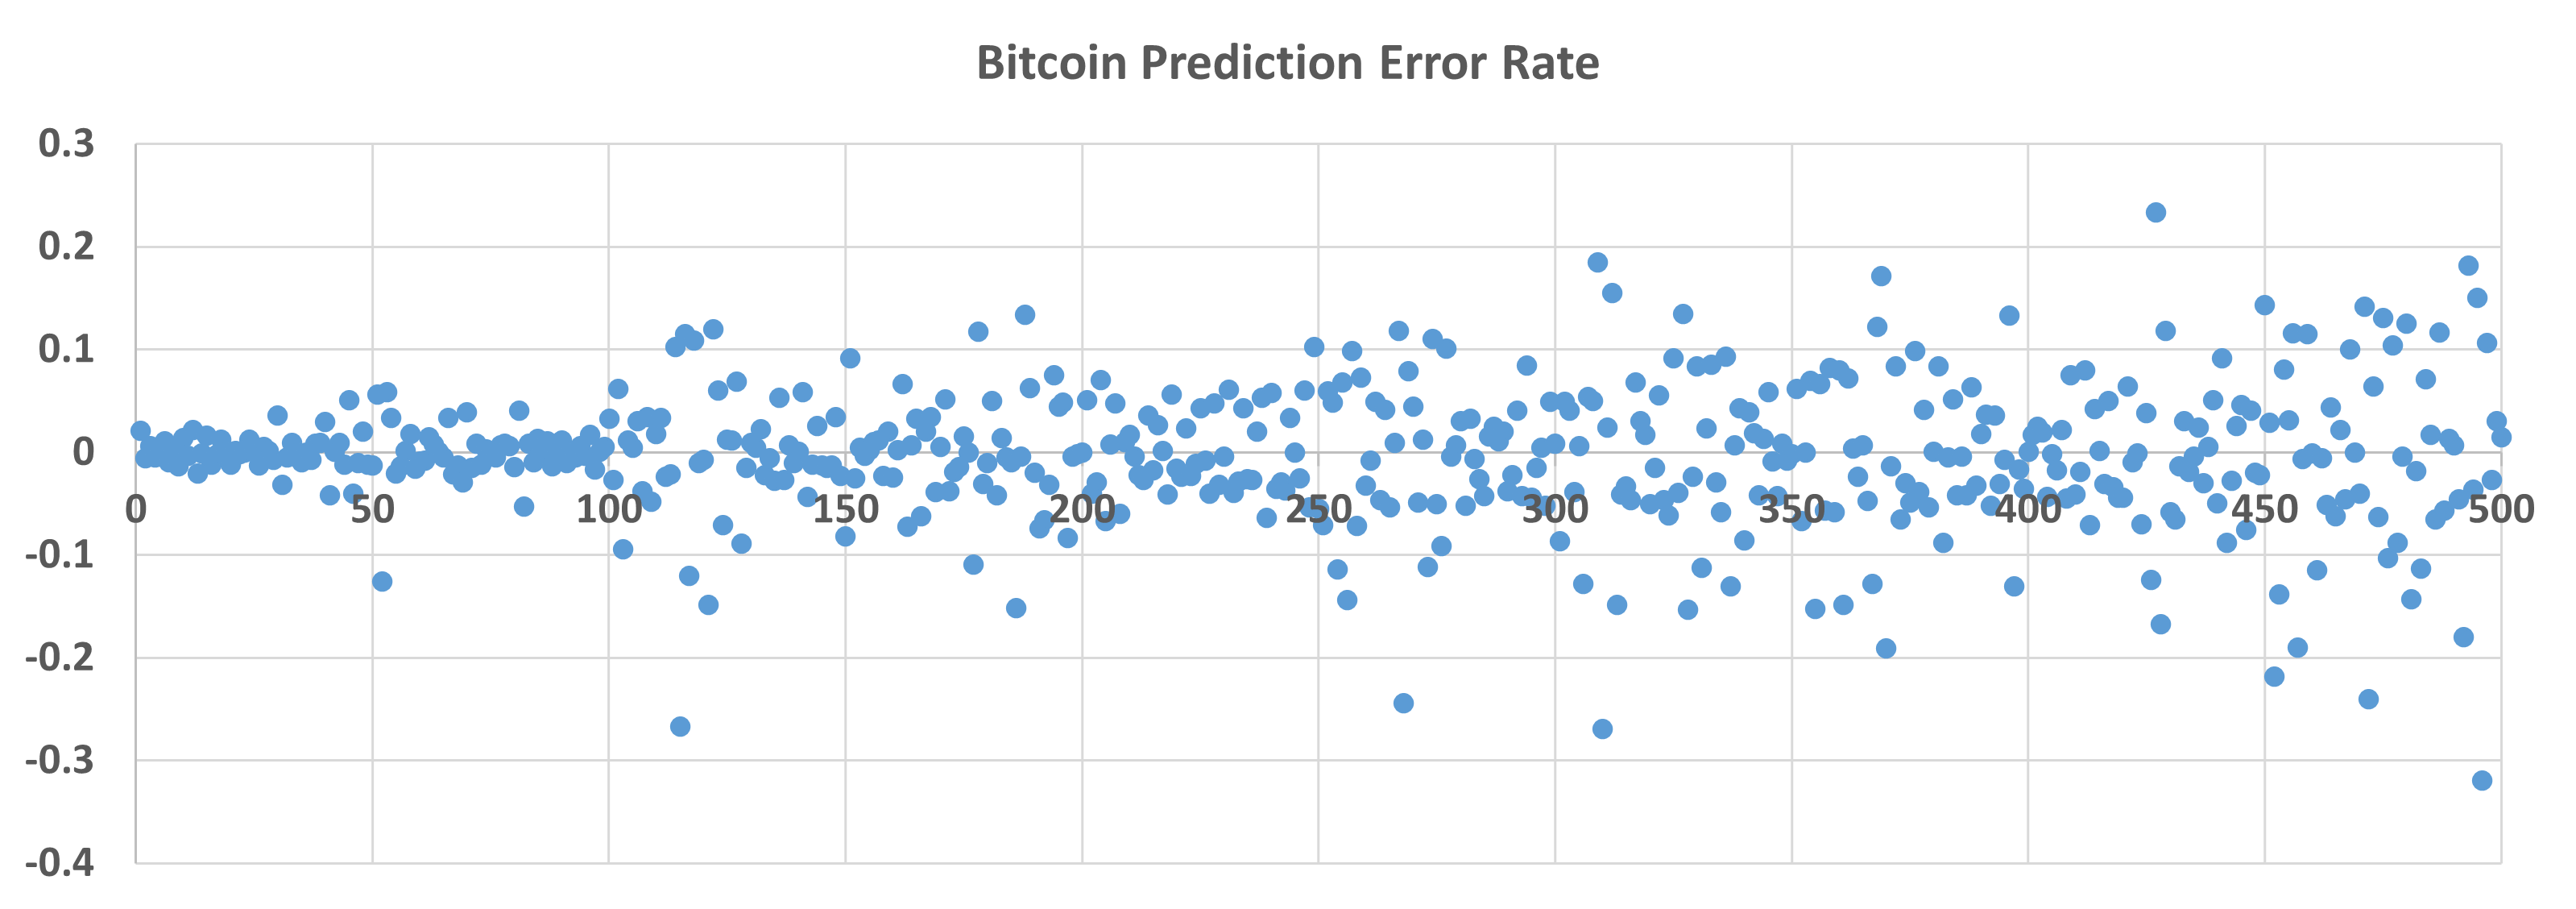
\includegraphics[width=0.8\linewidth]{figures/fig7}  
    \caption{Bitcoin Prediction Error Rate}
    \label{fig5:1}
\end{figure}
\newpage
\section{Prediction Model Construction: Interim and Late Stage Data}
\subsection{Building Monte Carlo Model}
When it comes to the 500th day, a sizable set of real historical price data has been accumulated. Our team decided to use the Monte Carlo model to predict the prices from the 501th day till the last day (1/24/2018~9/10/2021). Since the original historical price data do not meet the normal distribution requirement of MC model, we first applied Box-Cox transformation to make the price data set closely resemble a normal distribution, then used MC method to predict the next day's price, and finally applied inverse of the Box-Cox transformation to generate the ultimate predicted price. 
\subsubsection{Box-Cox transformation}
At first, Box-Cox transformation is applied to the historical price data set.
\begin{equation}
    y(\lambda)=\left\{
            \begin{aligned}
                \frac{y^\lambda-1}{\lambda},& &\lambda &\neq 0,\\
                \log(y),&&\lambda&=0.
            \end{aligned}
        \right.
\end{equation}
All values of $\lambda$, ranging from $-5$ to $5$, are considered and attempted for calculation. And the optimal value is selected from the trial result set; The selected optimal value set is the one which results in the best approximation of a normal distribution curve.

\subsubsection{Predicting Long-Term Data (after 500 days)}
Since $X,X_1,...,X_n$ are independently identically distributed random variables and $f$ is a function. $E[f(X)]<\infty$
\begin{equation}
    \lim_{n\rightarrow \infty}\frac{f(X_1)+...+f(X_n)}{n}=E[f(X)]
\end{equation}
with probability is 1. If $X$ has a probability density function $g(x)$, we have\begin{equation}
    E[f(X)]=\int_{\mathbb{R}^d}f(x)g(x)dx
\end{equation}
For $i$-the day, its compound annual return rate 
\begin{equation}
    \mu={\frac{p_{i-1}}{p_1}}^{\frac{365}{i-1}}-1,
\end{equation}
For the historical price $p_1,...,p_{i-1}$, let $D=\{d_1,...d_{i-2}\}$ where $d_j=\frac{p_j}{p_{j+1}}-1$, $j \in [1,i-2]\cap\mathbb{Z}$, and $\sigma_D$ is the standard deviation of $D$. We can get the annual volatility 
\begin{equation}
    v=\sigma_d\times\sqrt{365},
\end{equation}
and the $i+1$-th day prediction price
\begin{equation}
    p'_{i+1}\sim N(\frac{\mu}{i},\frac{v}{\sqrt{i}})
\end{equation}
\paragraph{}
For every time the model works, it will generate $p'_{i+1}$ randomly $10,000$ time for one prediction, and we would take the men value of the all outputs to work out the unique predicted price.
\subsubsection{Inverse Box-Cox Transformation}
After doing MC model prediction, we will transform it back using Inverse Box-Cox transformation
\begin{equation}
    y=(x\times \lambda+1)^{\frac{1}{\lambda}}
\end{equation}
After this process, the final predicted price is done.
\subsection{Predicting Price for gold and Bitcoin after the 500th day}
By repeating the whole process every day, we generate the predicted price set for 1/24/2018~9/10/2021, Figure \ref{fig8:1},Figure \ref{fig6:1} are Bitcoin prediction price and its error rate,Figure \ref{fig9:1},Figure \ref{fig7:1} are Gold prediction price and its error rate.
\begin{figure}[htp]
    \centering
    % include first image
    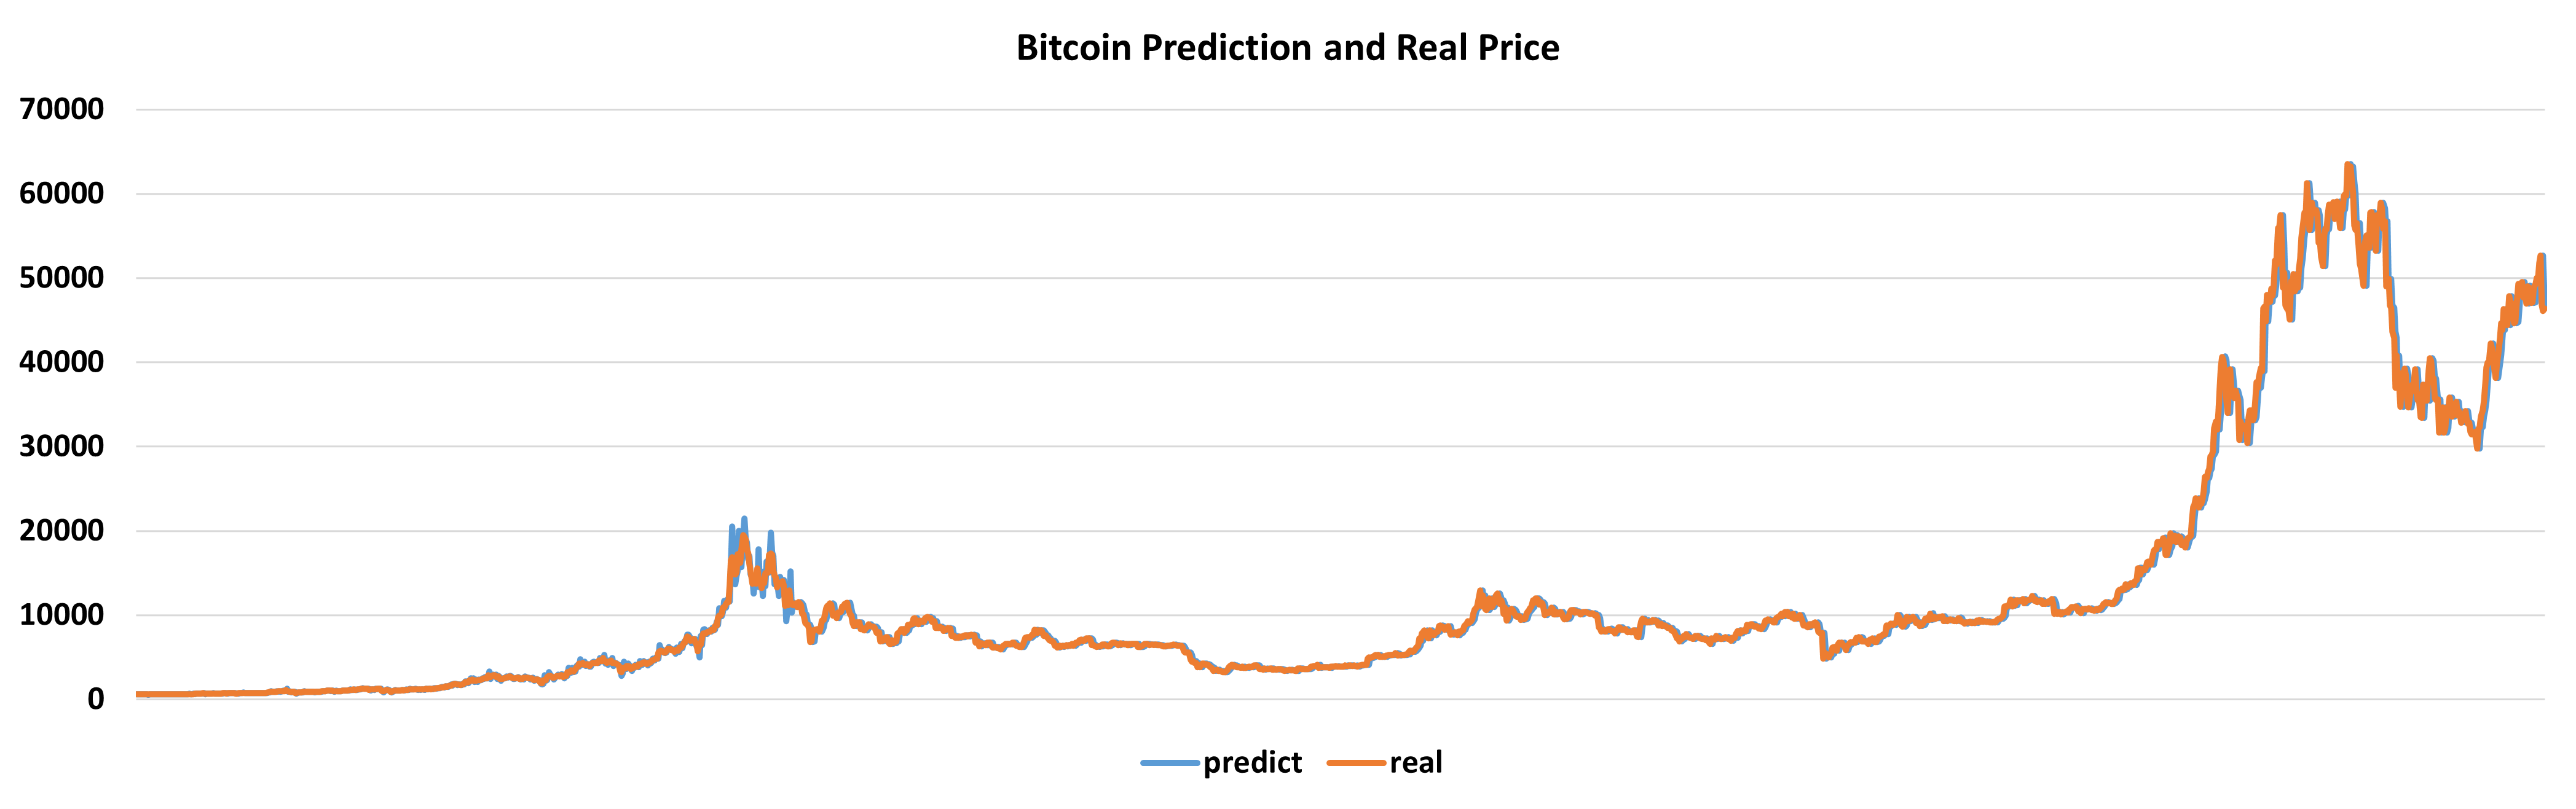
\includegraphics[width=0.8\linewidth]{figures/fig11_bitcoin_t.png}  
    \caption{Bitcoin Prediction Price}
    \label{fig8:1}
\end{figure}
\begin{figure}[htp]
    \centering
    % include first image
    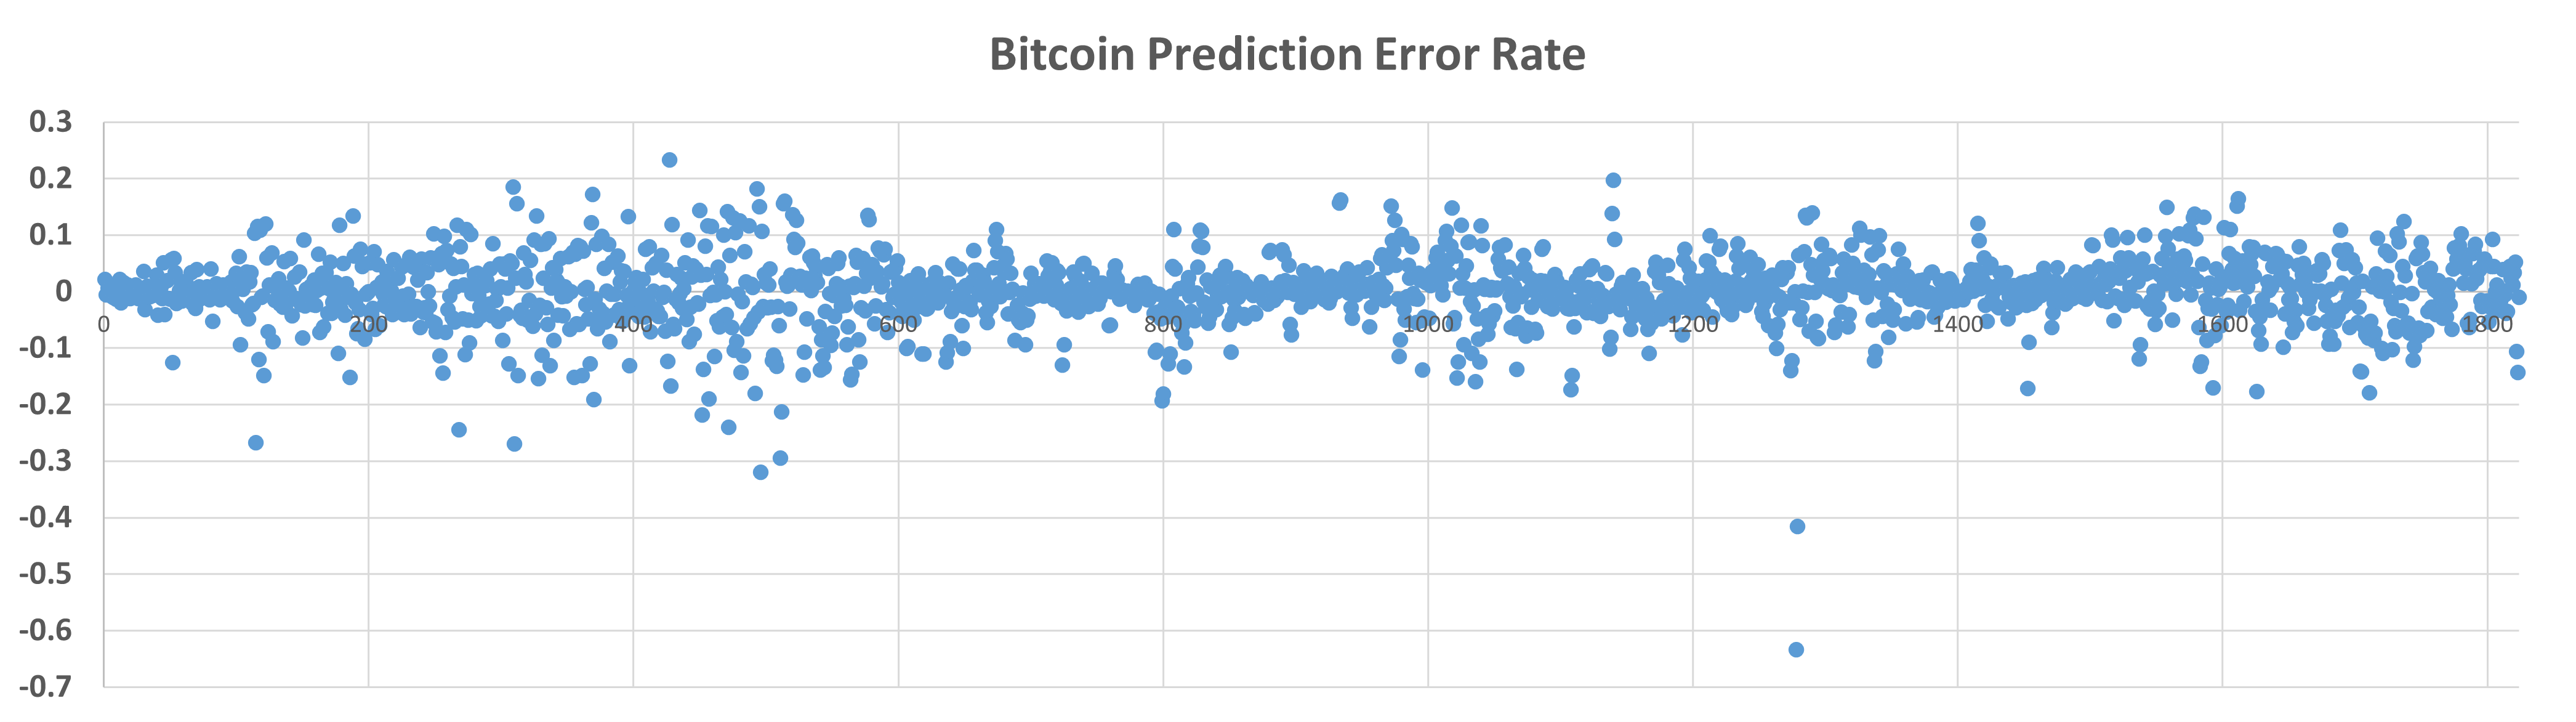
\includegraphics[width=0.8\linewidth]{figures/fig9.png}  
    \caption{Bitcoin Prediction Error Rate}
    \label{fig6:1}
\end{figure}
\begin{figure}[htp]
    \centering
    % include first image
    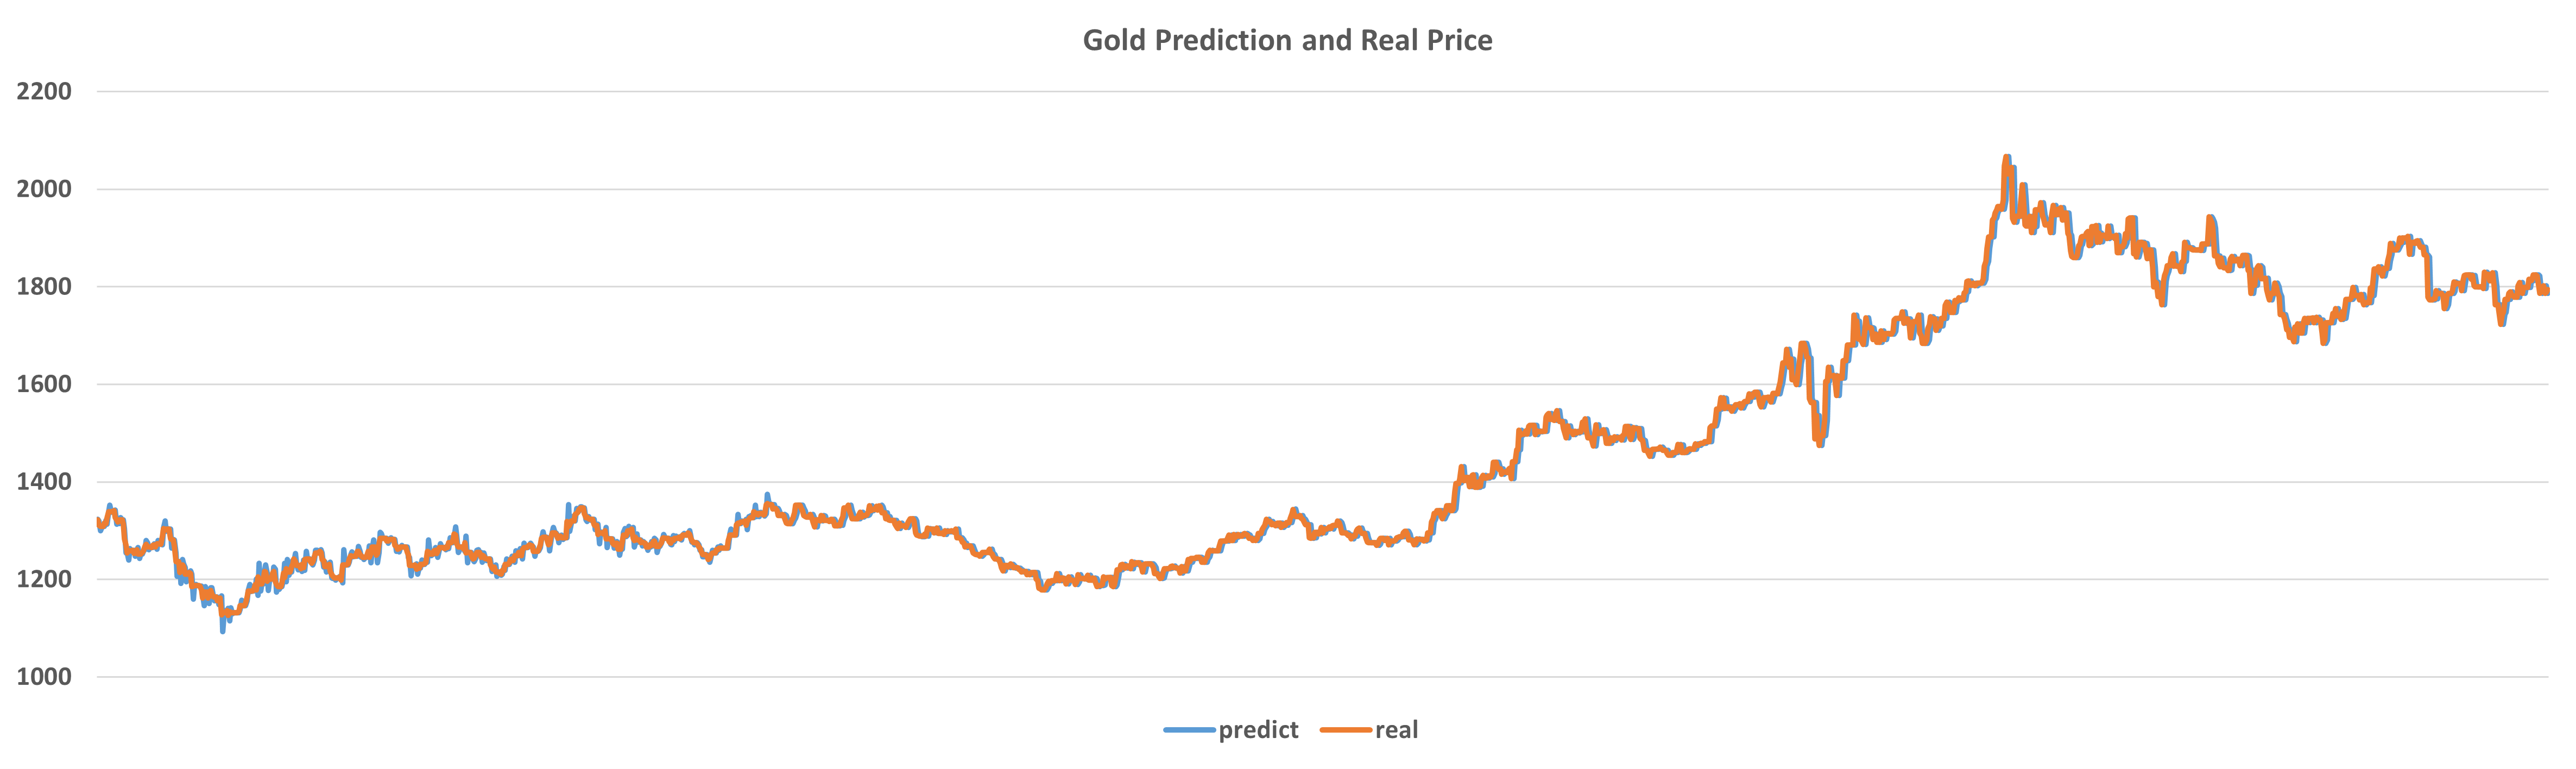
\includegraphics[width=0.8\linewidth]{figures/fig12_gold_t.png}  
    \caption{Gold Prediction Price}
    \label{fig9:1}
\end{figure}
\begin{figure}[htp]
    \centering
    % include first image
    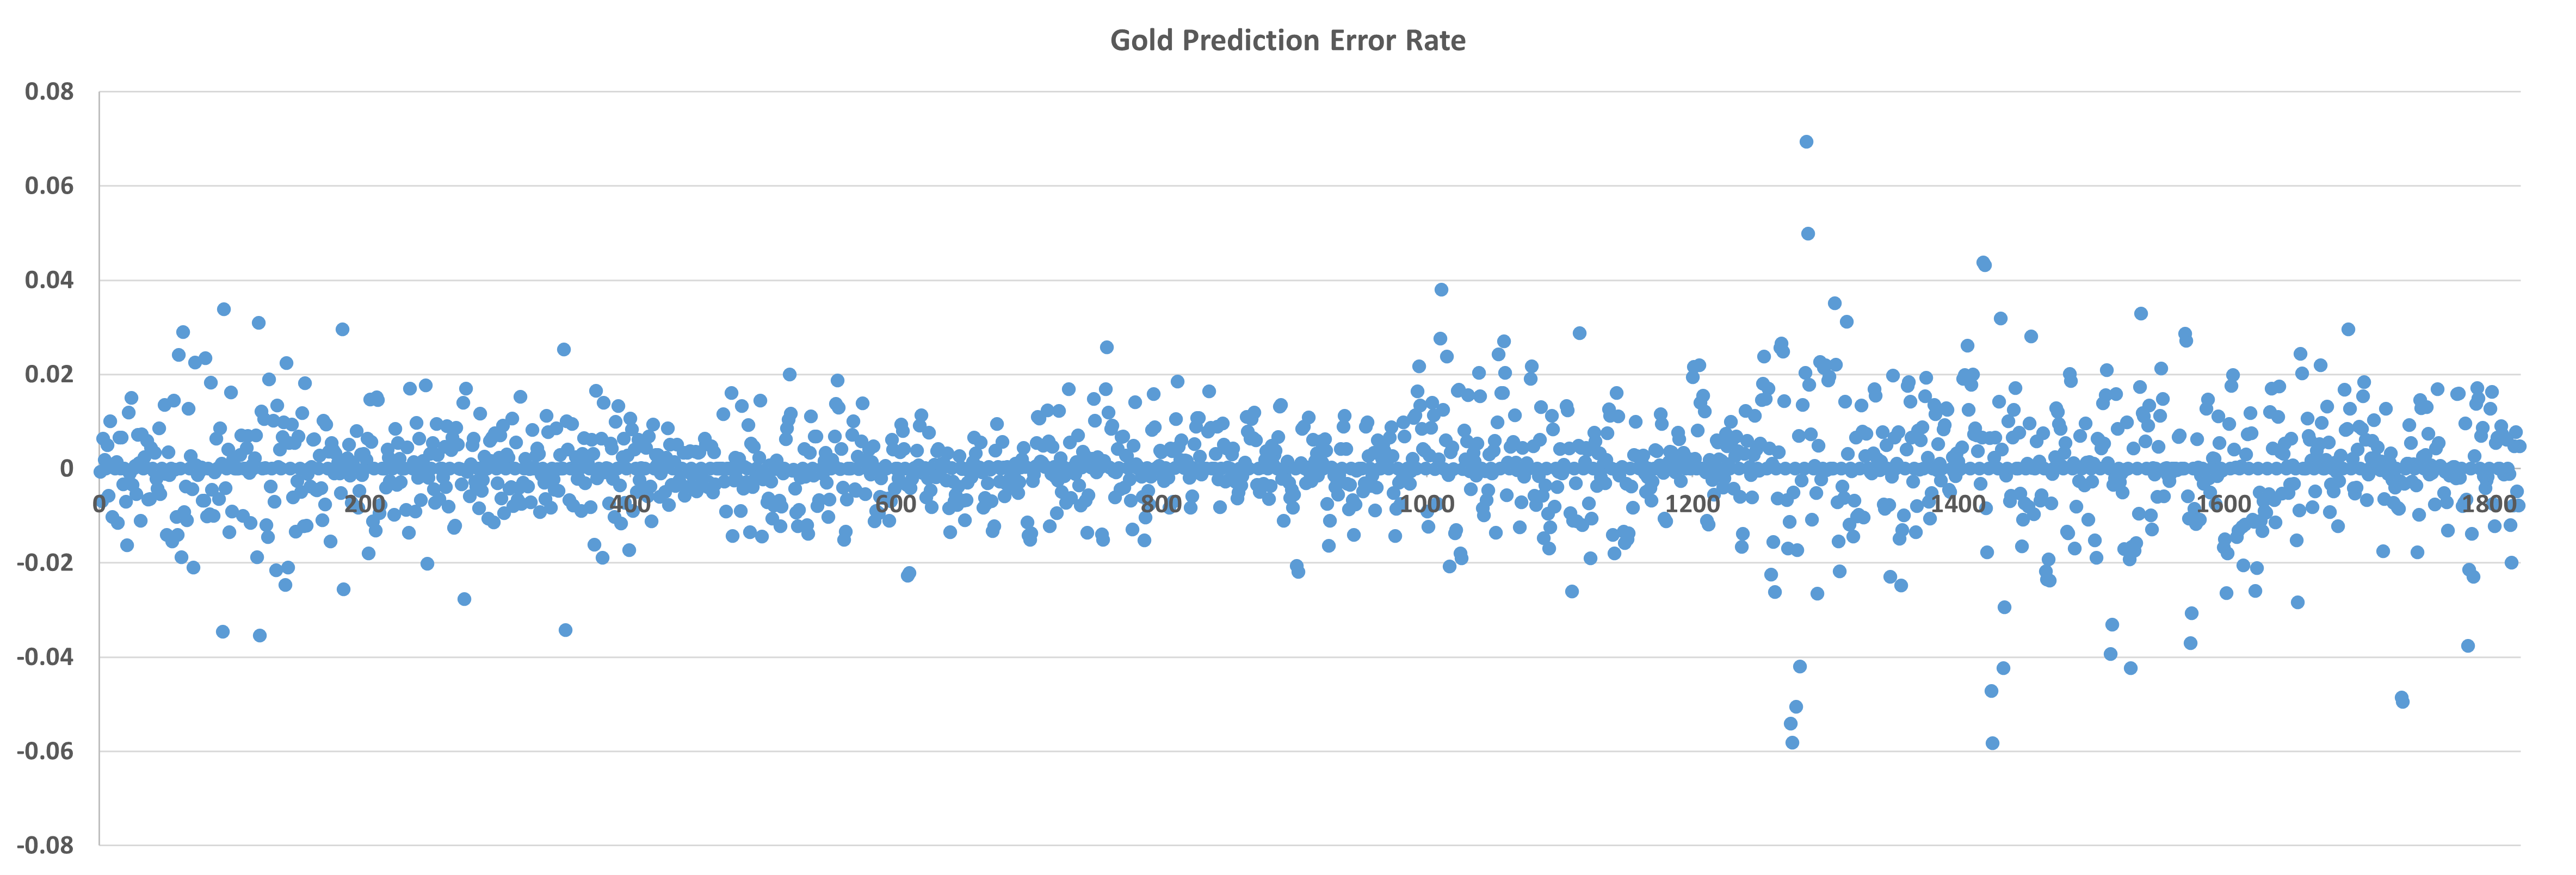
\includegraphics[width=0.8\linewidth]{figures/fig8.png}  
    \caption{Gold Prediction Error Rate}
    \label{fig7:1}
\end{figure}
\newpage
\section{Strategy Model Construction}
\subsection{Mentality in Building the Decision-making Model}
\paragraph{}
When building our model in the python program, whenever we are making a portfolio decision, we already know today's trading prices and tomorrow's predicted prices. So we decided to do three calculations simultaneously (Algorithm 1). 
\paragraph{}
\begin{algorithm}[H]
    \tcc{The revenue of selling all gold and Bitcoin and all in dollar}
    Dollar Revenue= sold(gold)+sold(Bitcoin)-value(gold)+value(Bitcoin)\\
    B Value=sold(BTC)-commission(BTC)\\
    G Value=sold(gold)-commission(gold)\\
    \tcc{The revenue of selling gold and all in Bitcoin}
    BTC Revenue= (G Value+Dollar-commission(BTC))*(Tmr BTC Price/Today BTC Price-1)\\
    \tcc{The revenue of selling BTC and all in gold}
    Gold Revenue= (B Value+Dollar-commission(gold))*(Tmr gold Price/Today gold Price-1)\\
    \tcc{Today's best strategy}
    max revenue=max(Dollar Revenue,BTC Revenue,Gold Revenue)\\
    \caption{Strategy}
\end{algorithm}
\newpage
Calculate the total value of your asset when you
\begin{itemize}
    \item[a.] sell all gold and Bitcoin holdings,
    \item[b.] sell all gold holdings and use all the USD in hand to buy BTC,
    \item[c.] sell all BTC holdings and use all the USD in hand to buy gold.
\end{itemize}
And we would select the largest value out of the three circumstances and take this strategy as the best portfolio decision for that day.
\paragraph{}
However, being the best portfolio strategy may not necessarily mean the best strategy for the overall situation.
Based on this, we need a transaction cost rate for each trade we make, and we need to deduct this transaction cost for each gain. The transaction cost of gold is 1\%,and the transaction cost of bitcoin is 2\%. If we trade frequently, we get less than the maximum total return. Our team decides not to trade when the return on each trade is less than the transaction cost to be paid.
\paragraph{}
So after several testing, our team set an earning threshold: if the best trading strategy today can't earn more than \$190, then the model will reject the strategy and choose not to trade on that day. Only when the predicted earning is over \$190 will the model accept the optimal strategy and do the trade. This practice is to reduce the loss of assets caused by frequent commission payments.

\subsection{How much is the initial \$1,000 investment worth on 9/10/2021 under our Model?}
By running our model, we calculated that the value of the asset on 9/10/2021 is \emph{\textbf{\$18929.4537}}, with a portfolio of 0 dollar, 0 ounce of gold and 0.408237837 Bitcoin.(Table 1 or Appendix)

\begin{table}
    % \tiny
    \caption{Final Result}
    \begin{center}
    \begin{tabular}{p{40pt}p{40pt}p{40pt}p{40pt}p{40pt}p{40pt}}
    \toprule
    Date & Value&(C,B,G)&Date & Value&(C,B,G)\\
    \midrule
    9/10/21&18810.9&(0,0.0,0.4)&9/11/21&18929.5&(0,0.0,0.4)\\
    \bottomrule 
    \end{tabular}
    \end{center}
    \end{table}
\section{Optimal Strategy Model and Sensitivity Analysis}
\subsection{Building the Markowitz Mean-Variance Model}
\paragraph{}
The Modern Portfolio Theory \cite{ref3} points out that investing in a portfolio with a relatively stable risk rate to maximize expected returns. And, based on the model that has some assumption:

\begin{itemize}
    \item there is no high correlation between the risky assets of the portfolio,
    \item investors are allowed to short sell stocks,
    \item the investor estimates the risk of the portfolio based on the expected return of the security.
\end{itemize}

\begin{table}
    \begin{center}
    \begin{tabular}{p{80pt}p{280pt}}
    \toprule
    Symbol       & Definitions \\
    \midrule
    $\sigma^2(\lambda_p)$       &  Variance of portfolio investment that is total portfolio investment risk. \\
    % \midrule
    $R_i$    & Standard deviation of daily volatility before $i$-th day. \\
    $\lambda_p$     & Portfolio investment income. \\
    $\omega_i$& Weight of the $i$-th investment. \\
    $\mu$& Expected return on portfolio investment.\\
    \bottomrule 
    \end{tabular}
    \end{center}
    \end{table}

\paragraph{}
Based on the solution to the optimal portfolio problem is the linear programming problem of finding the minimum $\sigma^2(\lambda_p)$ under the restriction that the fixed $\mu$ is known and $\omega_i$ is $1$. We get the model:
\begin{equation}
    \min \sigma^2(\lambda_p)=\frac{1}{2}\Omega^{T}\Sigma \Omega,
\end{equation}
\emph{s.t}
$$
    \left\{
        \begin{aligned}
            &\Omega^{T}R&=&\mu,\\
            &\Omega^T 1_n&=&1,\\
        \end{aligned}
    \right.
$$
where
$$
    % \left\{
        \begin{aligned}
            &\Sigma&=&\begin{bmatrix}
                cov(r_1,r_1)&cov(r_1,r_2)\\
                cov(r_2,r_1)&cov(r_2,r_2)
            \end{bmatrix},\\
            &\Omega&=&\begin{bmatrix}
                \omega_1\\
                \omega_2
            \end{bmatrix},\\
            &R&=&\begin{bmatrix}
                r_1\\
                r_2
            \end{bmatrix},\\
            &1_n&=&\begin{bmatrix}
                1\\
                1
            \end{bmatrix}.\\
        \end{aligned}
    % \right.
$$
By using the Lagrange multiplier to solve the solution, and Lagrange multiplier is defined by: For the case with n variables and k constraints, we have
\begin{equation}
    \mathcal{L}(x_1,...x_n,\lambda_1,...,\lambda_n)=f(x_1,...x_n)-\sum_{i=1}^k\lambda_ig_i(x_1,...x_n)
\end{equation}
Thus, we get the solution :
\begin{equation}
    \Omega^T=\begin{bmatrix}
        0.6&0.4
    \end{bmatrix}
\end{equation}
Table 2 shows that with different $mu$ we will have different the optimal solution of portfolio investment.
\begin{table}
    \caption{The optimal solution of portfolio investment with different $mu$}
    \begin{center}
    \begin{tabular}{p{40pt}p{40pt}p{40pt}p{40pt}p{40pt}p{40pt}p{40pt}p{40pt}}
    \toprule
    $\mu$\%       & 5\%&7.5\%&10\%&12.5\%&15\%&17.5\%&20\% \\
    \midrule
    Gold       & 0.459    &0.482&0.537&0.563&0.575&0.586&0.592 \\
    Bitcoin       & 0.541&0.518&0.463&0.437&0.425&0.414&0.408 \\
    \bottomrule 
    \end{tabular}
    \end{center}
    \end{table}
\subsection{How do transaction costs affect the strategy and results}
Figure \ref{fig:fig10} is our simulation result betwween commission rate and revenue rate. Revenue rate $r'(\alpha_B,\alpha_G)$ is defined by
\begin{equation}
    r'(\alpha_B,\alpha_G)=\frac{r(\alpha_B,\alpha_G)-r(2\%,1\%)}{r(2\%,1\%)}
\end{equation}
 where $r(\alpha_B,\alpha_G)$ is the final revenue under the Bitcoin commission rate $\alpha_B$ and gold commission rate $\alpha_G$
\begin{figure}[htp]
    \begin{subfigure}{.5\textwidth}
        \centering
        % include first image
        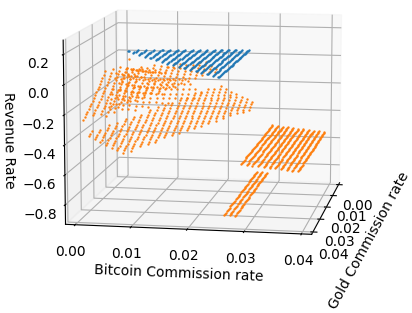
\includegraphics[width=0.9\linewidth]{figures/sen1.png}  
        \caption{}
        \label{fig10:1}
      \end{subfigure}
      \begin{subfigure}{.5\textwidth}
        \centering
        % include second image
        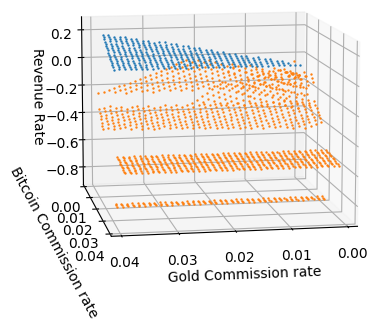
\includegraphics[width=0.9\linewidth]{figures/sne2.png}  
        \caption{}
        \label{fig10:2}
      \end{subfigure}
      \caption{Simulation Between Commission Rate and Revenue Rate}
      \label{fig:fig10}
\end{figure}
\paragraph{}
When the Bitcoin commission rate maintains a certain value, the gold commission rate between $0.1\%$ and $4\%$ can maintain a higher profit ratio than $(1\%, 2\%)$.
Similarly, when the Bitcoin commission ratio changes, the earning we can obtain is less than the earning at $(1\%, 2\%)$, and the gold commission ratio also has little effect on the final income. It can be seen that the sensitivity of our transaction model to the commission ratio of Bitcoin is much greater than the sensitivity of the commission ratio of gold.
\paragraph{}
Over the given five-year period, Bitcoin and gold prices have mostly been on the upswing, but Bitcoin prices have risen much more than gold. Likewise, according to the daily trading strategies generated by our analytical model, it can be seen that our model trades much more often between USD and Bitcoin compared with the trading frequency between USD and gold. This also indicates that in a market that continues to grow rapidly, Bitcoin, as a high-risk asset, has a higher value potential, so the transaction cost generated also affects our final income to a greater extent. It is conceivable that in a continuously shrinking market, as a stable asset, the transaction costs generated by gold will also affect our earnings to a greater extent.

\section{Evaluation of Model}
\subsection{Strengths}
\begin{itemize}
    \item We can make flexible adjustments to our trading strategy, since we are computing prediction values on a daily basis, which is a high frequency. Each time our model would use the latest stream of prices. By referring to the most recent daily price fluctuations, we can make more accurate predictions, thus better adjusting the trading strategy to maximize total earning.
    \item We did a case by case discussion, separating the whole trading period into two parts, the first 500 days and after 500 days, and applied two different models to achieve a better approximation.
    \item We set a trading baseline of \$190 and will not have a trade if the earning yield is less than the baseline. This ensures that each trade has a return that is greater than the cost of the trade,and ensures that each trade is executed at maximum return.
    \item By using BOPM for the early stage, the prediction calculation is simplified and the logic is more intuitive.
    \item The Monte Carlo Model is an empirical method based on the law of large numbers. When the quantity of experiments is large enough, the average value will be close to the theoretical value. Moreover, this model can estimate various risk factors of the portfolio, especially for non-linear portfolios that are difficult to estimate.
\end{itemize}
\subsection{Weaknesses}
\begin{itemize}
    \item Since the BOPM is based on the fact that today's price and next day's price are independent from each other, but in real life they are more or less inter-related.
    \item Since the Monte Carlo model requires a certain quantity of data to be accurate, a slightly large quantity of data upfront may affect the results of data prediction.
    \item The Monte Carlo model relies too much on particular historical data sets and ignores risk considerations, which may be affected by extreme values or structural changes.
\end{itemize}
\newpage
\section{Memorandum}
To: Trader\\
From: Team 2202067\\
Data: 21 Feb. 2022\\
Subject: Gold and Bitcoin Portfolio Decision Analysis\\
\noindent\rule[0.25\baselineskip]{\textwidth}{1pt}
\newline
We are the modeling team 2202067, today we are providing you with a comprehensive model that can be helpful in making investment decisions. Our model can not only predict future prices, but also work out optimal trading strategies and maximize your portfolio profit.  
\paragraph{}
Firstly, we would like to provide a brief overview of go-to-market: Bitcoin and gold. According to Statista (2022), the average daily trading volume of Bitcoin since 2017-2021 is about 280,000 times, and the average daily trading volume of gold is \$145.5 billion. This information shows that gold and Bitcoin have a large percentage of the market share and are popular commodities among investors.
\paragraph{}
Since your investment period is five years, which is quite a long time, we decided to use two prediction models in different time periods. Binomial Option Pricing Model for the first 500 days, and Monte Carlo Model for remaining days. The aim is to achieve higher accuracy. After predicting the prices, our model will generate the best trading strategy based on the past stream of daily prices as well as the next day's predicted price. 
\paragraph{}
However accurate our model is, please always note that the estimated risky rate of investment products can not accurately calculate the future price trend. 
\paragraph{}
Last but not least, what makes our model unique and competitive is that we did case by case discussion to work out more accurate predictions, also we set a earning baseline to prevent unnecessary duplication due to frequent commission payment.
\\ \hspace*{\fill} \\
FAQ:
\\ \hspace*{\fill} \\
Q: What factors may affect investment results?\\
A: Sudden social unrest, natural disasters, large public health security incidents, macroeconomic development, etc.
\\ \hspace*{\fill} \\
Q: Can you analyze why are gold and Bitcoin so popular among investors nowadays?\\
A: Gold is a value-preserving metal for investment, and the price of gold is at a relatively stable level. For Bitcoin, due to the development of science and technology, more market targets have shifted to the virtual world. Bitcoin is the origin of virtual currency, and the amount that can be mined is very small, so people may believe that If you own a certain amount of Bitcoin now, you can have an advantage in the future.\\

\emph{\textbf{**RISK WARNING: Discretion is advised for investments in the risky market.}}


\begin{thebibliography}{99}  
    \bibitem{ref5}HKEX, "Trading value, volume and number of deals", HKEX,21-Feb-2022. [Online]. Available: https://www.hkex.com.hk/. [Accessed: 21-Feb-2022]. 
    \bibitem{ref1}R. de Best, “Daily Bitcoin transactions 2017-2021,” Statista, 10-Jan-2022. [Online]. Available: https://www.statista.com/statistics/730806/daily-number-of-bitcoin-transactions/. [Accessed: 21-Feb-2022].   
    \bibitem{ref2}“Mean-variance portfolio theory,” CFA, FRM, and Actuarial Exams Study Notes, 14-Jul-2021. [Online]. Available: https://analystprep.com/study-notes/actuarial-exams/soa/ifm-investment-and-financial-markets/mean-variance-portfolio-theory/. [Accessed: 21-Feb-2022]. 
    \bibitem{ref3}“Modern portfolio theory (MPT),” Corporate Finance Institute, 05-Feb-2022. [Online]. Available: https://corporatefinanceinstitute.com/resources/knowledge/trading-investing/modern-portfolio-theory-mpt/. [Accessed: 21-Feb-2022].  
    \bibitem{ref4}Statista Research Department and J. , “Financial assets by Daily Trading Volume 2019,” Statista, 11-Jan-2022. [Online]. Available: https://www.statista.com/statistics/625422/daily-trading-volumes-of-major-financial-assets-worldwide/. [Accessed: 21-Feb-2022]. 
    \bibitem{ref6}E. Borgonovo, X. Lu, E. Plischke, O. Rakovec, and M. C. Hill, “Making the most out of a hydrological model data set: Sensitivity analyses to open the model black-box,” Water Resources Research, vol. 53, no. 9, pp. 7933-7950, 2017. 
\end{thebibliography}
\newpage
\section{Appendices}
% \addcontentsline{toc}{section}{Appendix}
\subsection{Monte Carlo Model Code}
\begin{lstlisting}
from scipy import stats,special
import numpy

def monte_carlo(bitcoin_price:list,n:int):
    past_bitcoin_price=bitcoin_price[:n]
    bitcoin_lm = stats.boxcox_normmax(past_bitcoin_price)
    bitcoin_nor = stats.boxcox(past_bitcoin_price, lmbda=bitcoin_lm)
    mu=(bitcoin_nor[-1]/bitcoin_nor[1])**(365/len(bitcoin_nor))-1
    t_array=[]
    for i in range(1,len(bitcoin_nor)):
        t_array=bitcoin_nor[i]/bitcoin_nor[i-1]-1
    vol=numpy.array(t_array).std()*numpy.sqrt(365)
    pe=bitcoin_price[n-1]
    res=[]
    for i in range(10000):
        res.append(numpy.random.normal(mu/len(bitcoin_nor), vol/numpy.sqrt(len(bitcoin_nor)),len(bitcoin_nor)))
    res=numpy.array(res)
    res=res.mean()
    res=special.inv_boxcox(res,bitcoin_lm)
    return (res)*pe   
\end{lstlisting}
\subsection{Binomial Option Pricing Model}
\begin{lstlisting}
import numpy

def bopm(bitcoin_price,n):
    past_bitcoin_price = bitcoin_price[n]
    r=(bitcoin_price[n]/bitcoin_price[n-1])-1
    t_array=[]
    for i in range(1,n):
        t_array=bitcoin_price[i]/bitcoin_price[i-1]-1
    vol=numpy.array(t_array).std()
    sigma=vol   
    u=numpy.e**sigma
    d=1/u
    a=numpy.e**r
    p=(a-d)/(u-d)
    res=p*past_bitcoin_price*u+(1-p)*past_bitcoin_price*d
    return res
\end{lstlisting}
\subsection{Trading Straregy}
\begin{lstlisting}
def strategy(today_bitcoin_price,tmr_bitcoin_price,
    today_gold_price,tmr_gold_price,
    gold_number,bitcoin_number,dollar_num):
    t = (bitcoin_number * today_bitcoin_price) / (1 + a_bitcoin)
    t += (gold_number * today_gold_price) / (1 + a_gold)
    dollar_prof = t-(bitcoin_number * today_bitcoin_price + gold_number * today_gold_price)
    if gold_number!=0:
        gold_prof=(gold_number*today_gold_price)*
                    (tmr_gold_price-today_gold_price)/
                    today_gold_price
        bitcoin_prof=(((gold_number*today_gold_price)/
                    (1+a_gold))/(1+a_bitcoin))*
                    (tmr_bitcoin_price-today_bitcoin_price)/
                    today_bitcoin_price
        flag=1
    elif bitcoin_number!=0:
        bitcoin_prof=(bitcoin_number*today_bitcoin_price)*
                    (tmr_bitcoin_price-today_bitcoin_price)/
                    today_bitcoin_price
        gold_prof=(((bitcoin_number*today_bitcoin_price)/
                    (1+a_bitcoin))/(1+a_gold))*
                    ((tmr_gold_price-today_gold_price)/
                    today_gold_price)
        flag=2
    else:
        gold_prof = (dollar_num / (1 + a_gold)) * ((tmr_gold_price - today_gold_price) / today_gold_price)
        bitcoin_prof = (dollar_num / (1 + a_bitcoin)) * (tmr_bitcoin_price - today_bitcoin_price) / today_bitcoin_price
        flag=3
    max_prof=max(max(gold_prof, bitcoin_prof), dollar_prof)
    if max_prof<190:
        return gold_number, bitcoin_number, dollar_num
    if max_prof==gold_prof:
        if flag==1:
            return gold_number, bitcoin_number, dollar_num
        if flag==2:
            gold_number+=(((bitcoin_number*today_bitcoin_price)/
                        (1+a_bitcoin))/(1+a_gold))/today_gold_price
            bitcoin_number=0
            return gold_number, bitcoin_number, dollar_num
        if flag==3:
            gold_number +=(dollar_num/(1+a_gold))/today_gold_price
            dollar_num=0
            return gold_number, bitcoin_number, dollar_num
        if max_prof==bitcoin_prof:
            if flag==1:
                bitcoin_number+=((gold_number*today_gold_price)/
                                (1+a_gold))/(1+a_bitcoin)/today_bitcoin_price
                gold_number=0
                return gold_number, bitcoin_number, dollar_num
            if flag==2:
                return gold_number, bitcoin_number, dollar_num
            if flag==3:
                bitcoin_number +=(dollar_num/(1+a_bitcoin))/today_bitcoin_price
                dollar_num=0
                return gold_number, bitcoin_number, dollar_num
        if max_prof==dollar_prof:
            if flag==1:
                dollar_num+=((gold_number*today_gold_price)/(1+a_gold))
                gold_number=0
                return gold_number, bitcoin_number, dollar_num
            if flag==2:
                dollar_num += ((bitcoin_number * today_bitcoin_price) / (1 + a_bitcoin))
                bitcoin_number = 0
                return gold_number, bitcoin_number, dollar_num
            if flag==3:
                return gold_number, bitcoin_number, dollar_num
\end{lstlisting}
%%%%%%%%%%%%%%%%%%%%%%%%%%%%%%
\subsection{The Data List of Portfolio and Accumulated Total Values}
\newpage
% \subsection{Strategy }
% \paragraph{}
\begin{table}
    \tiny
    \begin{center}
    \begin{tabular}{p{15pt}p{15pt}p{25pt}p{15pt}p{15pt}p{25pt}p{15pt}p{15pt}p{25pt}p{15pt}p{15pt}p{25pt}p{15pt}p{15pt}p{25pt}}
    \toprule
    Date & Value&(C,B,G)&Date & Value&(C,B,G)&Date & Value&(C,B,G)&Date & Value&(C,B,G)&Date & Value&(C,B,G)\\
    \midrule
    9/14/16&1000.0&(1000,0.0,0.0)&9/15/16&1000.0&(1000,0.0,0.0)&9/16/16&1000.0&(1000,0.0,0.0)&9/17/16&1000.0&(1000,0.0,0.0)&9/18/16&1000.0&(1000,0.0,0.0)\\
    9/19/16&1000.0&(1000,0.0,0.0)&9/20/16&1000.0&(1000,0.0,0.0)&9/21/16&1000.0&(1000,0.0,0.0)&9/22/16&1000.0&(1000,0.0,0.0)&9/23/16&1000.0&(1000,0.0,0.0)\\
    9/24/16&1000.0&(1000,0.0,0.0)&9/25/16&1000.0&(1000,0.0,0.0)&9/26/16&1000.0&(1000,0.0,0.0)&9/27/16&1000.0&(1000,0.0,0.0)&9/28/16&1000.0&(1000,0.0,0.0)\\
    9/29/16&1000.0&(1000,0.0,0.0)&9/30/16&1000.0&(1000,0.0,0.0)&10/1/16&1000.0&(1000,0.0,0.0)&10/2/16&1000.0&(1000,0.0,0.0)&10/3/16&1000.0&(1000,0.0,0.0)\\
    10/4/16&1000.0&(1000,0.0,0.0)&10/5/16&1000.0&(1000,0.0,0.0)&10/6/16&1000.0&(1000,0.0,0.0)&10/7/16&1000.0&(1000,0.0,0.0)&10/8/16&1000.0&(1000,0.0,0.0)\\
    10/9/16&1000.0&(1000,0.0,0.0)&10/10/16&1000.0&(1000,0.0,0.0)&10/11/16&1000.0&(1000,0.0,0.0)&10/12/16&1000.0&(1000,0.0,0.0)&10/13/16&1000.0&(1000,0.0,0.0)\\
    10/14/16&1000.0&(1000,0.0,0.0)&10/15/16&1000.0&(1000,0.0,0.0)&10/16/16&1000.0&(1000,0.0,0.0)&10/17/16&1000.0&(1000,0.0,0.0)&10/18/16&1000.0&(1000,0.0,0.0)\\
    10/19/16&1000.0&(1000,0.0,0.0)&10/20/16&1000.0&(1000,0.0,0.0)&10/21/16&1000.0&(1000,0.0,0.0)&10/22/16&1000.0&(1000,0.0,0.0)&10/23/16&1000.0&(1000,0.0,0.0)\\
    10/24/16&1000.0&(1000,0.0,0.0)&10/25/16&1000.0&(1000,0.0,0.0)&10/26/16&1000.0&(1000,0.0,0.0)&10/27/16&1000.0&(1000,0.0,0.0)&10/28/16&1000.0&(1000,0.0,0.0)\\
    10/29/16&1000.0&(1000,0.0,0.0)&10/30/16&1000.0&(1000,0.0,0.0)&10/31/16&1000.0&(1000,0.0,0.0)&11/1/16&1000.0&(1000,0.0,0.0)&11/2/16&1000.0&(1000,0.0,0.0)\\
    11/3/16&1000.0&(1000,0.0,0.0)&11/4/16&1000.0&(1000,0.0,0.0)&11/5/16&1000.0&(1000,0.0,0.0)&11/6/16&1000.0&(1000,0.0,0.0)&11/7/16&1000.0&(1000,0.0,0.0)\\
    11/8/16&1000.0&(1000,0.0,0.0)&11/9/16&1000.0&(1000,0.0,0.0)&11/10/16&1000.0&(1000,0.0,0.0)&11/11/16&1000.0&(1000,0.0,0.0)&11/12/16&1000.0&(1000,0.0,0.0)\\
    11/13/16&1000.0&(1000,0.0,0.0)&11/14/16&1000.0&(1000,0.0,0.0)&11/15/16&1000.0&(1000,0.0,0.0)&11/16/16&1000.0&(1000,0.0,0.0)&11/17/16&1000.0&(1000,0.0,0.0)\\
    11/18/16&1000.0&(1000,0.0,0.0)&11/19/16&1000.0&(1000,0.0,0.0)&11/20/16&1000.0&(1000,0.0,0.0)&11/21/16&1000.0&(1000,0.0,0.0)&11/22/16&1000.0&(1000,0.0,0.0)\\
    11/23/16&1000.0&(1000,0.0,0.0)&11/24/16&1000.0&(1000,0.0,0.0)&11/25/16&1000.0&(1000,0.0,0.0)&11/26/16&1000.0&(1000,0.0,0.0)&11/27/16&1000.0&(1000,0.0,0.0)\\
    11/28/16&1000.0&(1000,0.0,0.0)&11/29/16&1000.0&(1000,0.0,0.0)&11/30/16&1000.0&(1000,0.0,0.0)&12/1/16&1000.0&(1000,0.0,0.0)&12/2/16&1000.0&(1000,0.0,0.0)\\
    12/3/16&1000.0&(1000,0.0,0.0)&12/4/16&1000.0&(1000,0.0,0.0)&12/5/16&1000.0&(1000,0.0,0.0)&12/6/16&1000.0&(1000,0.0,0.0)&12/7/16&1000.0&(1000,0.0,0.0)\\
    12/8/16&1000.0&(1000,0.0,0.0)&12/9/16&1000.0&(1000,0.0,0.0)&12/10/16&1000.0&(1000,0.0,0.0)&12/11/16&1000.0&(1000,0.0,0.0)&12/12/16&1000.0&(1000,0.0,0.0)\\
    12/13/16&1000.0&(1000,0.0,0.0)&12/14/16&1000.0&(1000,0.0,0.0)&12/15/16&1000.0&(1000,0.0,0.0)&12/16/16&1000.0&(1000,0.0,0.0)&12/17/16&1000.0&(1000,0.0,0.0)\\
    12/18/16&1000.0&(1000,0.0,0.0)&12/19/16&1000.0&(1000,0.0,0.0)&12/20/16&1000.0&(1000,0.0,0.0)&12/21/16&1000.0&(1000,0.0,0.0)&12/22/16&1000.0&(1000,0.0,0.0)\\
    12/23/16&1000.0&(1000,0.0,0.0)&12/24/16&1000.0&(1000,0.0,0.0)&12/25/16&1000.0&(1000,0.0,0.0)&12/26/16&1000.0&(1000,0.0,0.0)&12/27/16&1000.0&(1000,0.0,0.0)\\
    12/28/16&1000.0&(1000,0.0,0.0)&12/29/16&1000.0&(1000,0.0,0.0)&12/30/16&1000.0&(1000,0.0,0.0)&12/31/16&1000.0&(1000,0.0,0.0)&1/1/17&1000.0&(1000,0.0,0.0)\\
    1/2/17&1000.0&(1000,0.0,0.0)&1/3/17&1000.0&(1000,0.0,0.0)&1/4/17&1000.0&(1000,0.0,0.0)&1/5/17&1000.0&(1000,0.0,0.0)&1/6/17&1000.0&(1000,0.0,0.0)\\
    1/7/17&1000.0&(1000,0.0,0.0)&1/8/17&1000.0&(1000,0.0,0.0)&1/9/17&1000.0&(1000,0.0,0.0)&1/10/17&1000.0&(1000,0.0,0.0)&1/11/17&1000.0&(1000,0.0,0.0)\\
    1/12/17&1000.0&(1000,0.0,0.0)&1/13/17&1000.0&(1000,0.0,0.0)&1/14/17&1000.0&(1000,0.0,0.0)&1/15/17&1000.0&(1000,0.0,0.0)&1/16/17&1000.0&(1000,0.0,0.0)\\
    1/17/17&1000.0&(1000,0.0,0.0)&1/18/17&1000.0&(1000,0.0,0.0)&1/19/17&1000.0&(1000,0.0,0.0)&1/20/17&1000.0&(1000,0.0,0.0)&1/21/17&1000.0&(1000,0.0,0.0)\\
    1/22/17&1000.0&(1000,0.0,0.0)&1/23/17&1000.0&(1000,0.0,0.0)&1/24/17&1000.0&(1000,0.0,0.0)&1/25/17&1000.0&(1000,0.0,0.0)&1/26/17&1000.0&(1000,0.0,0.0)\\
    1/27/17&1000.0&(1000,0.0,0.0)&1/28/17&1000.0&(1000,0.0,0.0)&1/29/17&1000.0&(1000,0.0,0.0)&1/30/17&1000.0&(1000,0.0,0.0)&1/31/17&1000.0&(1000,0.0,0.0)\\
    2/1/17&1000.0&(1000,0.0,0.0)&2/2/17&1000.0&(1000,0.0,0.0)&2/3/17&1000.0&(1000,0.0,0.0)&2/4/17&1000.0&(1000,0.0,0.0)&2/5/17&1000.0&(1000,0.0,0.0)\\
    2/6/17&1000.0&(1000,0.0,0.0)&2/7/17&1000.0&(1000,0.0,0.0)&2/8/17&1000.0&(1000,0.0,0.0)&2/9/17&1000.0&(1000,0.0,0.0)&2/10/17&1000.0&(1000,0.0,0.0)\\
    2/11/17&1000.0&(1000,0.0,0.0)&2/12/17&1000.0&(1000,0.0,0.0)&2/13/17&1000.0&(1000,0.0,0.0)&2/14/17&1000.0&(1000,0.0,0.0)&2/15/17&1000.0&(1000,0.0,0.0)\\
    2/16/17&1000.0&(1000,0.0,0.0)&2/17/17&1000.0&(1000,0.0,0.0)&2/18/17&1000.0&(1000,0.0,0.0)&2/19/17&1000.0&(1000,0.0,0.0)&2/20/17&1000.0&(1000,0.0,0.0)\\
    2/21/17&1000.0&(1000,0.0,0.0)&2/22/17&1000.0&(1000,0.0,0.0)&2/23/17&1000.0&(1000,0.0,0.0)&2/24/17&1000.0&(1000,0.0,0.0)&2/25/17&1000.0&(1000,0.0,0.0)\\
    2/26/17&1000.0&(1000,0.0,0.0)&2/27/17&1000.0&(1000,0.0,0.0)&2/28/17&1000.0&(1000,0.0,0.0)&3/1/17&1000.0&(1000,0.0,0.0)&3/2/17&1000.0&(1000,0.0,0.0)\\
    3/3/17&1000.0&(1000,0.0,0.0)&3/4/17&1000.0&(1000,0.0,0.0)&3/5/17&1000.0&(1000,0.0,0.0)&3/6/17&1000.0&(1000,0.0,0.0)&3/7/17&1000.0&(1000,0.0,0.0)\\
    3/8/17&1000.0&(1000,0.0,0.0)&3/9/17&1000.0&(1000,0.0,0.0)&3/10/17&1000.0&(1000,0.0,0.0)&3/11/17&1000.0&(1000,0.0,0.0)&3/12/17&1000.0&(1000,0.0,0.0)\\
    3/13/17&1000.0&(1000,0.0,0.0)&3/14/17&1000.0&(1000,0.0,0.0)&3/15/17&1000.0&(1000,0.0,0.0)&3/16/17&1000.0&(1000,0.0,0.0)&3/17/17&1000.0&(1000,0.0,0.0)\\
    3/18/17&1000.0&(1000,0.0,0.0)&3/19/17&1000.0&(1000,0.0,0.0)&3/20/17&1000.0&(1000,0.0,0.0)&3/21/17&1000.0&(1000,0.0,0.0)&3/22/17&1000.0&(1000,0.0,0.0)\\
    3/23/17&1000.0&(1000,0.0,0.0)&3/24/17&1000.0&(1000,0.0,0.0)&3/25/17&1000.0&(1000,0.0,0.0)&3/26/17&1000.0&(1000,0.0,0.0)&3/27/17&1000.0&(1000,0.0,0.0)\\
    3/28/17&1000.0&(1000,0.0,0.0)&3/29/17&1000.0&(1000,0.0,0.0)&3/30/17&1000.0&(1000,0.0,0.0)&3/31/17&1000.0&(1000,0.0,0.0)&4/1/17&1000.0&(1000,0.0,0.0)\\
    4/2/17&1000.0&(1000,0.0,0.0)&4/3/17&1000.0&(1000,0.0,0.0)&4/4/17&1000.0&(1000,0.0,0.0)&4/5/17&1000.0&(1000,0.0,0.0)&4/6/17&1000.0&(1000,0.0,0.0)\\
    4/7/17&1000.0&(1000,0.0,0.0)&4/8/17&1000.0&(1000,0.0,0.0)&4/9/17&1000.0&(1000,0.0,0.0)&4/10/17&1000.0&(1000,0.0,0.0)&4/11/17&1000.0&(1000,0.0,0.0)\\
    4/12/17&1000.0&(1000,0.0,0.0)&4/13/17&1000.0&(1000,0.0,0.0)&4/14/17&1000.0&(1000,0.0,0.0)&4/15/17&1000.0&(1000,0.0,0.0)&4/16/17&1000.0&(1000,0.0,0.0)\\
    4/17/17&1000.0&(1000,0.0,0.0)&4/18/17&1000.0&(1000,0.0,0.0)&4/19/17&1000.0&(1000,0.0,0.0)&4/20/17&1000.0&(1000,0.0,0.0)&4/21/17&1000.0&(1000,0.0,0.0)\\
    4/22/17&1000.0&(1000,0.0,0.0)&4/23/17&1000.0&(1000,0.0,0.0)&4/24/17&1000.0&(1000,0.0,0.0)&4/25/17&1000.0&(1000,0.0,0.0)&4/26/17&1000.0&(1000,0.0,0.0)\\
    4/27/17&1000.0&(1000,0.0,0.0)&4/28/17&1000.0&(1000,0.0,0.0)&4/29/17&1000.0&(1000,0.0,0.0)&4/30/17&1000.0&(1000,0.0,0.0)&5/1/17&1000.0&(1000,0.0,0.0)\\
    5/2/17&1000.0&(1000,0.0,0.0)&5/3/17&1000.0&(1000,0.0,0.0)&5/4/17&1000.0&(1000,0.0,0.0)&5/5/17&1000.0&(1000,0.0,0.0)&5/6/17&1000.0&(1000,0.0,0.0)\\
    5/7/17&1000.0&(1000,0.0,0.0)&5/8/17&1000.0&(1000,0.0,0.0)&5/9/17&1000.0&(1000,0.0,0.0)&5/10/17&1000.0&(1000,0.0,0.0)&5/11/17&1000.0&(1000,0.0,0.0)\\
    5/12/17&1000.0&(1000,0.0,0.0)&5/13/17&1000.0&(1000,0.0,0.0)&5/14/17&1000.0&(1000,0.0,0.0)&5/15/17&1000.0&(1000,0.0,0.0)&5/16/17&1000.0&(1000,0.0,0.0)\\
    5/17/17&1000.0&(1000,0.0,0.0)&5/18/17&1000.0&(1000,0.0,0.0)&5/19/17&1000.0&(1000,0.0,0.0)&5/20/17&1000.0&(1000,0.0,0.0)&5/21/17&1000.0&(1000,0.0,0.0)\\
    5/22/17&1000.0&(1000,0.0,0.0)&5/23/17&1000.0&(1000,0.0,0.0)&5/24/17&1000.0&(1000,0.0,0.0)&5/25/17&1000.0&(1000,0.0,0.0)&5/26/17&1000.0&(1000,0.0,0.0)\\
    5/27/17&1000.0&(1000,0.0,0.0)&5/28/17&1000.0&(1000,0.0,0.0)&5/29/17&1000.0&(1000,0.0,0.0)&5/30/17&1000.0&(1000,0.0,0.0)&5/31/17&1000.0&(1000,0.0,0.0)\\
    6/1/17&1000.0&(1000,0.0,0.0)&6/2/17&1000.0&(1000,0.0,0.0)&6/3/17&1000.0&(1000,0.0,0.0)&6/4/17&1000.0&(1000,0.0,0.0)&6/5/17&1000.0&(1000,0.0,0.0)\\
    6/6/17&1000.0&(1000,0.0,0.0)&6/7/17&1000.0&(1000,0.0,0.0)&6/8/17&1000.0&(1000,0.0,0.0)&6/9/17&1000.0&(1000,0.0,0.0)&6/10/17&1000.0&(1000,0.0,0.0)\\
    6/11/17&1000.0&(1000,0.0,0.0)&6/12/17&1000.0&(1000,0.0,0.0)&6/13/17&1000.0&(1000,0.0,0.0)&6/14/17&1000.0&(1000,0.0,0.0)&6/15/17&1000.0&(1000,0.0,0.0)\\
    6/16/17&1000.0&(1000,0.0,0.0)&6/17/17&1000.0&(1000,0.0,0.0)&6/18/17&1000.0&(1000,0.0,0.0)&6/19/17&1000.0&(1000,0.0,0.0)&6/20/17&1000.0&(1000,0.0,0.0)\\
    6/21/17&1000.0&(1000,0.0,0.0)&6/22/17&1000.0&(1000,0.0,0.0)&6/23/17&1000.0&(1000,0.0,0.0)&6/24/17&1000.0&(1000,0.0,0.0)&6/25/17&1000.0&(1000,0.0,0.0)\\
    6/26/17&1000.0&(1000,0.0,0.0)&6/27/17&1000.0&(1000,0.0,0.0)&6/28/17&1000.0&(1000,0.0,0.0)&6/29/17&1000.0&(1000,0.0,0.0)&6/30/17&1000.0&(1000,0.0,0.0)\\
    7/1/17&1000.0&(1000,0.0,0.0)&7/2/17&1000.0&(1000,0.0,0.0)&7/3/17&1000.0&(1000,0.0,0.0)&7/4/17&1000.0&(1000,0.0,0.0)&7/5/17&1000.0&(1000,0.0,0.0)\\
    7/6/17&1000.0&(1000,0.0,0.0)&7/7/17&1000.0&(1000,0.0,0.0)&7/8/17&1000.0&(1000,0.0,0.0)&7/9/17&1000.0&(1000,0.0,0.0)&7/10/17&1000.0&(1000,0.0,0.0)\\
    7/11/17&1000.0&(1000,0.0,0.0)&7/12/17&1000.0&(1000,0.0,0.0)&7/13/17&1000.0&(1000,0.0,0.0)&7/14/17&1000.0&(1000,0.0,0.0)&7/15/17&1000.0&(1000,0.0,0.0)\\
    7/16/17&1000.0&(1000,0.0,0.0)&7/17/17&1000.0&(1000,0.0,0.0)&7/18/17&1000.0&(1000,0.0,0.0)&7/19/17&1190.3&(0,0.0,0.5)&7/20/17&1161.9&(0,0.0,0.5)\\
    7/21/17&1162.1&(0,0.0,0.5)&7/22/17&1376.1&(0,0.0,0.5)&7/23/17&1440.4&(0,0.0,0.5)&7/24/17&1449.6&(0,0.0,0.5)&7/25/17&1411.8&(0,0.0,0.5)\\
    7/26/17&1313.9&(0,0.0,0.5)&7/27/17&1315.6&(0,0.0,0.5)&7/28/17&1358.3&(0,0.0,0.5)&7/29/17&1427.1&(0,0.0,0.5)&7/30/17&1428.7&(0,0.0,0.5)\\
    7/31/17&1408.8&(0,0.0,0.5)&8/1/17&1470.6&(0,0.0,0.5)&8/2/17&1468.8&(0,0.0,0.5)&8/3/17&1381.9&(0,0.0,0.5)&8/4/17&1433.5&(0,0.0,0.5)\\
    8/5/17&1431.4&(0,0.0,0.5)&8/6/17&1651.0&(0,0.0,0.5)&8/7/17&1668.7&(0,0.0,0.5)&8/8/17&1646.9&(0,0.0,0.5)&8/9/17&1773.8&(0,0.0,0.5)\\
    8/10/17&1722.4&(0,0.0,0.5)&8/11/17&1713.7&(0,0.0,0.5)&8/12/17&1863.6&(0,0.0,0.5)&8/13/17&1976.6&(0,0.0,0.5)&8/14/17&1984.7&(0,0.0,0.5)\\
    8/15/17&2197.3&(0,0.0,0.5)&8/16/17&2163.5&(0,0.0,0.5)&8/17/17&2144.5&(0,0.0,0.5)&8/18/17&2220.8&(0,0.0,0.5)&8/19/17&2119.1&(0,0.0,0.5)\\
    8/20/17&2105.9&(0,0.0,0.5)&8/21/17&2133.2&(0,0.0,0.5)&8/22/17&2074.6&(0,0.0,0.5)&8/23/17&2045.1&(0,0.0,0.5)&8/24/17&2141.9&(0,0.0,0.5)\\
    8/25/17&2226.7&(0,0.0,0.5)&8/26/17&2222.4&(0,0.0,0.5)&8/27/17&2237.1&(0,0.0,0.5)&8/28/17&2233.9&(0,0.0,0.5)&8/29/17&2226.1&(0,0.0,0.5)\\
    8/30/17&2364.1&(0,0.0,0.5)&8/31/17&2357.4&(0,0.0,0.5)&9/1/17&2351.0&(0,0.0,0.5)&9/2/17&2519.9&(0,0.0,0.5)&9/3/17&2349.9&(0,0.0,0.5)\\
    9/4/17&2352.6&(0,0.0,0.5)&9/5/17&2228.7&(0,0.0,0.5)&9/6/17&2302.9&(0,0.0,0.5)&9/7/17&2249.7&(0,0.0,0.5)&9/8/17&2388.0&(0,0.0,0.5)\\
    9/9/17&2211.6&(0,0.0,0.5)&9/10/17&2212.3&(0,0.0,0.5)&9/11/17&2221.4&(0,0.0,0.5)&9/12/17&2179.4&(0,0.0,0.5)&9/13/17&2154.0&(0,0.0,0.5)\\
    9/14/17&2032.3&(0,0.0,0.5)&9/15/17&1703.1&(0,0.0,0.5)&9/16/17&1650.1&(0,0.0,0.5)&9/17/17&1930.9&(0,0.0,0.5)&9/18/17&1921.9&(0,0.0,0.5)\\
    9/19/17&1887.2&(0,0.0,0.5)&9/20/17&2023.1&(0,0.0,0.5)&9/21/17&2040.6&(0,0.0,0.5)&9/22/17&1998.0&(0,0.0,0.5)&9/23/17&1866.2&(0,0.0,0.5)\\
    9/24/17&1937.4&(0,0.0,0.5)&9/25/17&1938.1&(0,0.0,0.5)&9/26/17&2022.7&(0,0.0,0.5)&9/27/17&2006.1&(0,0.0,0.5)&9/28/17&1991.1&(0,0.0,0.5)\\
    9/29/17&2155.8&(0,0.0,0.5)&9/30/17&2151.5&(0,0.0,0.5)&10/1/17&2136.4&(0,0.0,0.5)&10/2/17&2237.2&(0,0.0,0.5)&10/3/17&2250.6&(0,0.0,0.5)\\
    10/4/17&2254.3&(0,0.0,0.5)&10/5/17&2167.7&(0,0.0,0.5)&10/6/17&2226.0&(0,0.0,0.5)&10/7/17&2215.6&(0,0.0,0.5)&10/8/17&2245.1&(0,0.0,0.5)\\
    10/9/17&2361.1&(0,0.0,0.5)&10/10/17&2362.9&(0,0.0,0.5)&10/11/17&2453.5&(0,0.0,0.5)&10/12/17&2472.6&(0,0.0,0.5)&10/13/17&2473.9&(0,0.0,0.5)\\
    10/14/17&2854.4&(0,0.0,0.5)&10/15/17&2944.5&(0,0.0,0.5)&10/16/17&2988.9&(0,0.0,0.5)&10/17/17&2930.1&(0,0.0,0.5)&10/18/17&2874.9&(0,0.0,0.5)\\
    10/19/17&2870.3&(0,0.0,0.5)&10/20/17&2938.5&(0,0.0,0.5)&10/21/17&3067.7&(0,0.0,0.5)&10/22/17&3071.3&(0,0.0,0.5)&10/23/17&3069.6&(0,0.0,0.5)\\
    10/24/17&3014.6&(0,0.0,0.5)&10/25/17&3027.2&(0,0.0,0.5)&10/26/17&2908.7&(0,0.0,0.5)&10/27/17&3023.4&(0,0.0,0.5)&10/28/17&3021.7&(0,0.0,0.5)\\
    10/29/17&2963.7&(0,0.0,0.5)&10/30/17&3158.0&(0,0.0,0.5)&10/31/17&3148.2&(0,0.0,0.5)&11/1/17&3277.6&(0,0.0,0.5)&11/2/17&3419.5&(0,0.0,0.5)\\
    11/3/17&3464.0&(0,0.0,0.5)&11/4/17&3692.7&(0,0.0,0.5)&11/5/17&3815.7&(0,0.0,0.5)&11/6/17&3779.0&(0,0.0,0.5)&11/7/17&3585.6&(0,0.0,0.5)\\
    11/8/17&3638.5&(0,0.0,0.5)&11/9/17&3657.3&(0,0.0,0.5)&11/10/17&3672.3&(0,0.0,0.5)&11/11/17&3447.3&(0,0.0,0.5)&11/12/17&3370.2&(0,0.0,0.5)\\
    11/13/17&2932.7&(0,0.0,0.5)&11/14/17&3360.5&(0,0.0,0.5)&11/15/17&3331.5&(0,0.0,0.5)&11/16/17&3745.9&(0,0.0,0.5)&11/17/17&4009.4&(0,0.0,0.5)\\
    11/18/17&4037.0&(0,0.0,0.5)&11/19/17&4010.5&(0,0.0,0.5)&11/20/17&4108.2&(0,0.0,0.5)&11/21/17&4129.8&(0,0.0,0.5)&11/22/17&4135.0&(0,0.0,0.5)\\
    11/23/17&4241.8&(0,0.0,0.5)&11/24/17&4225.7&(0,0.0,0.5)&11/25/17&4233.1&(0,0.0,0.5)&11/26/17&4467.2&(0,0.0,0.5)&11/27/17&4498.7&(0,0.0,0.5)\\
    11/28/17&4985.8&(0,0.0,0.5)&11/29/17&5106.0&(0,0.0,0.5)&11/30/17&5088.8&(0,0.0,0.5)&12/1/17&5206.0&(0,0.0,0.5)&12/2/17&5583.8&(0,0.0,0.5)\\
    12/3/17&5581.8&(0,0.0,0.5)&12/4/17&5814.0&(0,0.0,0.5)&12/5/17&5943.4&(0,0.0,0.5)&12/6/17&5946.7&(0,0.0,0.5)&12/7/17&6947.0&(0,0.0,0.5)\\
    12/8/17&8466.1&(0,0.0,0.5)&12/9/17&8650.2&(0,0.0,0.5)&12/10/17&7768.8&(0,0.0,0.5)&12/11/17&7628.8&(0,0.0,0.5)&12/12/17&7730.9&(0,0.0,0.5)\\
    12/13/17&8863.4&(0,0.0,0.5)&12/14/17&8623.3&(0,0.0,0.5)&12/15/17&8338.0&(0,0.0,0.5)&12/16/17&9117.6&(0,0.0,0.5)&12/17/17&10003.5&(0,0.0,0.5)\\
    12/18/17&9891.3&(0,0.0,0.5)&12/19/17&9728.1&(0,0.0,0.5)&12/20/17&9099.8&(0,0.0,0.5)&12/21/17&8918.1&(0,0.0,0.5)&12/22/17&8233.0&(0,0.0,0.5)\\
    12/23/17&7793.5&(0,0.0,0.5)&12/24/17&7067.9&(0,0.0,0.5)&12/25/17&7156.4&(0,0.0,0.5)&12/26/17&7243.6&(0,0.0,0.5)&12/27/17&7049.6&(0,0.0,0.5)\\
    12/28/17&7997.9&(0,0.0,0.5)&12/29/17&7377.8&(0,0.0,0.5)&12/30/17&7292.3&(0,0.0,0.5)&12/31/17&6780.1&(0,0.0,0.5)&1/1/18&7267.5&(0,0.0,0.5)\\
    1/2/18&7077.9&(0,0.0,0.5)&1/3/18&7698.6&(0,0.0,0.5)&1/4/18&7722.9&(0,0.0,0.5)&1/5/18&7715.7&(0,0.0,0.5)&1/6/18&8810.9&(0,0.0,0.5)\\
    1/7/18&8885.4&(0,0.0,0.5)&1/8/18&8801.6&(0,0.0,0.5)&1/9/18&7832.0&(0,0.0,0.5)&1/10/18&7548.9&(0,0.0,0.5)&1/11/18&7406.9&(0,0.0,0.5)\\
    1/12/18&6821.7&(0,0.0,0.5)&1/13/18&7137.8&(0,0.0,0.5)&1/14/18&7075.4&(0,0.0,0.5)&1/15/18&7107.1&(0,0.0,0.5)&1/16/18&7188.8&(0,0.0,0.5)\\
    \bottomrule 
    \end{tabular}
    \end{center}
    \end{table}

    \begin{table}
        \tiny
        \begin{center}
        \begin{tabular}{p{15pt}p{15pt}p{25pt}p{15pt}p{15pt}p{25pt}p{15pt}p{15pt}p{25pt}p{15pt}p{15pt}p{25pt}p{15pt}p{15pt}p{25pt}}
        \toprule
        Date & Value&(C,B,G)&Date & Value&(C,B,G)&Date & Value&(C,B,G)&Date & Value&(C,B,G)&Date & Value&(C,B,G)\\
        \midrule
        1/17/18&6953.8&(0,0.0,0.5)&1/18/18&5703.4&(0,0.0,0.5)&1/19/18&5820.6&(0,0.0,0.5)&1/20/18&5733.1&(0,0.0,0.5)&1/21/18&6644.2&(0,0.0,0.5)\\
        1/22/18&5902.6&(0,0.0,0.5)&1/23/18&5906.8&(0,0.0,0.5)&1/24/18&5757.8&(0,0.0,0.5)&1/25/18&5788.2&(0,0.0,0.5)&1/26/18&5844.5&(0,0.0,0.5)\\
        1/27/18&5627.9&(0,0.0,0.5)&1/28/18&5912.6&(0,0.0,0.5)&1/29/18&5864.7&(0,0.0,0.5)&1/30/18&5752.5&(0,0.0,0.5)&1/31/18&5224.8&(0,0.0,0.5)\\
        2/1/18&5172.7&(0,0.0,0.5)&2/2/18&4660.0&(0,0.0,0.5)&2/3/18&4567.0&(0,0.0,0.5)&2/4/18&4541.8&(0,0.0,0.5)&2/5/18&4309.8&(0,0.0,0.5)\\
        2/6/18&3508.6&(0,0.0,0.5)&2/7/18&3553.0&(0,0.0,0.5)&2/8/18&4155.6&(0,0.0,0.5)&2/9/18&4227.7&(0,0.0,0.5)&2/10/18&4230.0&(0,0.0,0.5)\\
        2/11/18&4268.4&(0,0.0,0.5)&2/12/18&4280.5&(0,0.0,0.5)&2/13/18&4139.2&(0,0.0,0.5)&2/14/18&4411.0&(0,0.0,0.5)&2/15/18&4789.0&(0,0.0,0.5)\\
        2/16/18&4859.3&(0,0.0,0.5)&2/17/18&5195.6&(0,0.0,0.5)&2/18/18&5562.3&(0,0.0,0.5)&2/19/18&5687.4&(0,0.0,0.5)&2/20/18&5700.3&(0,0.0,0.5)\\
        2/21/18&5843.7&(0,0.0,0.5)&2/22/18&5769.6&(0,0.0,0.5)&2/23/18&5095.0&(0,0.0,0.5)&2/24/18&5213.5&(0,0.0,0.5)&2/25/18&5218.2&(0,0.0,0.5)\\
        2/26/18&4974.7&(0,0.0,0.5)&2/27/18&5309.2&(0,0.0,0.5)&2/28/18&5294.3&(0,0.0,0.5)&3/1/18&5320.3&(0,0.0,0.5)&3/2/18&5648.2&(0,0.0,0.5)\\
        3/3/18&5608.1&(0,0.0,0.5)&3/4/18&5811.1&(0,0.0,0.5)&3/5/18&5864.1&(0,0.0,0.5)&3/6/18&5908.6&(0,0.0,0.5)&3/7/18&5521.9&(0,0.0,0.5)\\
        3/8/18&5190.9&(0,0.0,0.5)&3/9/18&5089.6&(0,0.0,0.5)&3/10/18&4663.1&(0,0.0,0.5)&3/11/18&4487.0&(0,0.0,0.5)&3/12/18&4503.1&(0,0.0,0.5)\\
        3/13/18&4711.1&(0,0.0,0.5)&3/14/18&4696.7&(0,0.0,0.5)&3/15/18&4696.1&(0,0.0,0.5)&3/16/18&4288.0&(0,0.0,0.5)&3/17/18&4376.4&(0,0.0,0.5)\\
        3/18/18&4257.1&(0,0.0,0.5)&3/19/18&4192.2&(0,0.0,0.5)&3/20/18&4315.7&(0,0.0,0.5)&3/21/18&4415.0&(0,0.0,0.5)&3/22/18&4590.5&(0,0.0,0.5)\\
        3/23/18&4458.5&(0,0.0,0.5)&3/24/18&4476.4&(0,0.0,0.5)&3/25/18&4444.1&(0,0.0,0.5)&3/26/18&4421.0&(0,0.0,0.5)&3/27/18&4339.2&(0,0.0,0.5)\\
        3/28/18&4040.8&(0,0.0,0.5)&3/29/18&4084.0&(0,0.0,0.5)&3/30/18&4079.0&(0,0.0,0.5)&3/31/18&3531.0&(0,0.0,0.5)&4/1/18&3558.2&(0,0.0,0.5)\\
        4/2/18&3559.2&(0,0.0,0.5)&4/3/18&3609.6&(0,0.0,0.5)&4/4/18&3801.8&(0,0.0,0.5)&4/5/18&3810.1&(0,0.0,0.5)&4/6/18&3502.2&(0,0.0,0.5)\\
        4/7/18&3388.0&(0,0.0,0.5)&4/8/18&3403.8&(0,0.0,0.5)&4/9/18&3600.3&(0,0.0,0.5)&4/10/18&3437.0&(0,0.0,0.5)&4/11/18&3480.6&(0,0.0,0.5)\\
        4/12/18&3553.4&(0,0.0,0.5)&4/13/18&4026.2&(0,0.0,0.5)&4/14/18&4074.3&(0,0.0,0.5)&4/15/18&4123.0&(0,0.0,0.5)&4/16/18&4279.1&(0,0.0,0.5)\\
        4/17/18&4293.1&(0,0.0,0.5)&4/18/18&4050.6&(0,0.0,0.5)&4/19/18&4188.9&(0,0.0,0.5)&4/20/18&4194.6&(0,0.0,0.5)&4/21/18&4541.8&(0,0.0,0.5)\\
        4/22/18&4518.4&(0,0.0,0.5)&4/23/18&4581.7&(0,0.0,0.5)&4/24/18&4583.4&(0,0.0,0.5)&4/25/18&4902.3&(0,0.0,0.5)&4/26/18&4955.0&(0,0.0,0.5)\\
        4/27/18&4749.9&(0,0.0,0.5)&4/28/18&4622.6&(0,0.0,0.5)&4/29/18&4580.7&(0,0.0,0.5)&4/30/18&4788.8&(0,0.0,0.5)&5/1/18&4750.5&(0,0.0,0.5)\\
        5/2/18&4740.2&(0,0.0,0.5)&5/3/18&4730.9&(0,0.0,0.5)&5/4/18&4945.3&(0,0.0,0.5)&5/5/18&5003.8&(0,0.0,0.5)&5/6/18&5029.5&(0,0.0,0.5)\\
        5/7/18&4940.6&(0,0.0,0.5)&5/8/18&4941.3&(0,0.0,0.5)&5/9/18&4734.6&(0,0.0,0.5)&5/10/18&4782.5&(0,0.0,0.5)&5/11/18&4776.6&(0,0.0,0.5)\\
        5/12/18&4344.8&(0,0.0,0.5)&5/13/18&4352.8&(0,0.0,0.5)&5/14/18&4342.1&(0,0.0,0.5)&5/15/18&4438.8&(0,0.0,0.5)&5/16/18&4366.7&(0,0.0,0.5)\\
        5/17/18&4346.0&(0,0.0,0.5)&5/18/18&4158.7&(0,0.0,0.5)&5/19/18&4227.4&(0,0.0,0.5)&5/20/18&4226.9&(0,0.0,0.5)&5/21/18&4364.6&(0,0.0,0.5)\\
        5/22/18&4302.1&(0,0.0,0.5)&5/23/18&4307.8&(0,0.0,0.5)&5/24/18&3876.4&(0,0.0,0.5)&5/25/18&3881.7&(0,0.0,0.5)&5/26/18&3887.2&(0,0.0,0.5)\\
        5/27/18&3767.2&(0,0.0,0.5)&5/28/18&3776.9&(0,0.0,0.5)&5/29/18&3768.0&(0,0.0,0.5)&5/30/18&3827.2&(0,0.0,0.5)&5/31/18&3789.0&(0,0.0,0.5)\\
        6/1/18&3789.7&(0,0.0,0.5)&6/2/18&3865.8&(0,0.0,0.5)&6/3/18&3922.2&(0,0.0,0.5)&6/4/18&3918.1&(0,0.0,0.5)&6/5/18&3847.9&(0,0.0,0.5)\\
        6/6/18&3907.1&(0,0.0,0.5)&6/7/18&3909.0&(0,0.0,0.5)&6/8/18&3938.2&(0,0.0,0.5)&6/9/18&3909.4&(0,0.0,0.5)&6/10/18&3907.0&(0,0.0,0.5)\\
        6/11/18&3476.8&(0,0.0,0.5)&6/12/18&3527.5&(0,0.0,0.5)&6/13/18&3529.3&(0,0.0,0.5)&6/14/18&3240.2&(0,0.0,0.5)&6/15/18&3410.2&(0,0.0,0.5)\\
        6/16/18&3405.2&(0,0.0,0.5)&6/17/18&3339.6&(0,0.0,0.5)&6/18/18&3316.5&(0,0.0,0.5)&6/19/18&3306.9&(0,0.0,0.5)&6/20/18&3456.3&(0,0.0,0.5)\\
        6/21/18&3444.9&(0,0.0,0.5)&6/22/18&3468.6&(0,0.0,0.5)&6/23/18&3248.8&(0,0.0,0.5)&6/24/18&3150.9&(0,0.0,0.5)&6/25/18&3165.7&(0,0.0,0.5)\\
        6/26/18&3186.7&(0,0.0,0.5)&6/27/18&3190.4&(0,0.0,0.5)&6/28/18&3128.2&(0,0.0,0.5)&6/29/18&3133.6&(0,0.0,0.5)&6/30/18&3031.4&(0,0.0,0.5)\\
        7/1/18&3192.8&(0,0.0,0.5)&7/2/18&3270.5&(0,0.0,0.5)&7/3/18&3317.3&(0,0.0,0.5)&7/4/18&3399.6&(0,0.0,0.5)&7/5/18&3382.6&(0,0.0,0.5)\\
        7/6/18&3387.8&(0,0.0,0.5)&7/7/18&3363.2&(0,0.0,0.5)&7/8/18&3383.1&(0,0.0,0.5)&7/9/18&3464.8&(0,0.0,0.5)&7/10/18&3449.7&(0,0.0,0.5)\\
        7/11/18&3340.3&(0,0.0,0.5)&7/12/18&3271.8&(0,0.0,0.5)&7/13/18&3285.1&(0,0.0,0.5)&7/14/18&3203.6&(0,0.0,0.5)&7/15/18&3201.9&(0,0.0,0.5)\\
        7/16/18&3205.9&(0,0.0,0.5)&7/17/18&3342.1&(0,0.0,0.5)&7/18/18&3524.5&(0,0.0,0.5)&7/19/18&3756.3&(0,0.0,0.5)&7/20/18&3794.6&(0,0.0,0.5)\\
        7/21/18&3810.9&(0,0.0,0.5)&7/22/18&3763.1&(0,0.0,0.5)&7/23/18&3822.8&(0,0.0,0.5)&7/24/18&3945.2&(0,0.0,0.5)&7/25/18&3958.1&(0,0.0,0.5)\\
        7/26/18&4233.1&(0,0.0,0.5)&7/27/18&4200.4&(0,0.0,0.5)&7/28/18&4073.4&(0,0.0,0.5)&7/29/18&4197.8&(0,0.0,0.5)&7/30/18&4210.2&(0,0.0,0.5)\\
        7/31/18&4217.6&(0,0.0,0.5)&8/1/18&4061.6&(0,0.0,0.5)&8/2/18&3884.1&(0,0.0,0.5)&8/3/18&3903.0&(0,0.0,0.5)&8/4/18&3793.6&(0,0.0,0.5)\\
        8/5/18&3718.4&(0,0.0,0.5)&8/6/18&3597.0&(0,0.0,0.5)&8/7/18&3585.1&(0,0.0,0.5)&8/8/18&3587.9&(0,0.0,0.5)&8/9/18&3446.7&(0,0.0,0.5)\\
        8/10/18&3281.8&(0,0.0,0.5)&8/11/18&3281.6&(0,0.0,0.5)&8/12/18&3149.5&(0,0.0,0.5)&8/13/18&3237.8&(0,0.0,0.5)&8/14/18&3256.3&(0,0.0,0.5)\\
        8/15/18&3207.6&(0,0.0,0.5)&8/16/18&3264.3&(0,0.0,0.5)&8/17/18&3254.0&(0,0.0,0.5)&8/18/18&3238.7&(0,0.0,0.5)&8/19/18&3302.3&(0,0.0,0.5)\\
        8/20/18&3285.5&(0,0.0,0.5)&8/21/18&3327.9&(0,0.0,0.5)&8/22/18&3284.1&(0,0.0,0.5)&8/23/18&3373.3&(0,0.0,0.5)&8/24/18&3260.1&(0,0.0,0.5)\\
        8/25/18&3357.1&(0,0.0,0.5)&8/26/18&3447.3&(0,0.0,0.5)&8/27/18&3457.0&(0,0.0,0.5)&8/28/18&3447.2&(0,0.0,0.5)&8/29/18&3591.3&(0,0.0,0.5)\\
        8/30/18&3631.4&(0,0.0,0.5)&8/31/18&3556.7&(0,0.0,0.5)&9/1/18&3582.0&(0,0.0,0.5)&9/2/18&3600.9&(0,0.0,0.5)&9/3/18&3718.5&(0,0.0,0.5)\\
        9/4/18&3725.1&(0,0.0,0.5)&9/5/18&3727.3&(0,0.0,0.5)&9/6/18&3649.3&(0,0.0,0.5)&9/7/18&3300.5&(0,0.0,0.5)&9/8/18&3335.3&(0,0.0,0.5)\\
        9/9/18&3266.0&(0,0.0,0.5)&9/10/18&3225.2&(0,0.0,0.5)&9/11/18&3201.9&(0,0.0,0.5)&9/12/18&3230.2&(0,0.0,0.5)&9/13/18&3218.3&(0,0.0,0.5)\\
        9/14/18&3245.5&(0,0.0,0.5)&9/15/18&3334.3&(0,0.0,0.5)&9/16/18&3344.3&(0,0.0,0.5)&9/17/18&3346.2&(0,0.0,0.5)&9/18/18&3283.7&(0,0.0,0.5)\\
        9/19/18&3230.4&(0,0.0,0.5)&9/20/18&3253.9&(0,0.0,0.5)&9/21/18&3293.0&(0,0.0,0.5)&9/22/18&3421.9&(0,0.0,0.5)&9/23/18&3466.1&(0,0.0,0.5)\\
        9/24/18&3442.7&(0,0.0,0.5)&9/25/18&3406.2&(0,0.0,0.5)&9/26/18&3377.5&(0,0.0,0.5)&9/27/18&3318.6&(0,0.0,0.5)&9/28/18&3352.9&(0,0.0,0.5)\\
        9/29/18&3430.2&(0,0.0,0.5)&9/30/18&3360.6&(0,0.0,0.5)&10/1/18&3382.5&(0,0.0,0.5)&10/2/18&3391.7&(0,0.0,0.5)&10/3/18&3366.9&(0,0.0,0.5)\\
        10/4/18&3319.6&(0,0.0,0.5)&10/5/18&3326.4&(0,0.0,0.5)&10/6/18&3369.9&(0,0.0,0.5)&10/7/18&3376.5&(0,0.0,0.5)&10/8/18&3372.5&(0,0.0,0.5)\\
        10/9/18&3395.6&(0,0.0,0.5)&10/10/18&3397.2&(0,0.0,0.5)&10/11/18&3399.8&(0,0.0,0.5)&10/12/18&3205.8&(0,0.0,0.5)&10/13/18&3211.9&(0,0.0,0.5)\\
        10/14/18&3204.9&(0,0.0,0.5)&10/15/18&3231.8&(0,0.0,0.5)&10/16/18&3310.4&(0,0.0,0.5)&10/17/18&3385.6&(0,0.0,0.5)&10/18/18&3384.1&(0,0.0,0.5)\\
        10/19/18&3369.6&(0,0.0,0.5)&10/20/18&3339.7&(0,0.0,0.5)&10/21/18&3329.0&(0,0.0,0.5)&10/22/18&3350.9&(0,0.0,0.5)&10/23/18&3337.2&(0,0.0,0.5)\\
        10/24/18&3325.2&(0,0.0,0.5)&10/25/18&3339.0&(0,0.0,0.5)&10/26/18&3329.5&(0,0.0,0.5)&10/27/18&3321.3&(0,0.0,0.5)&10/28/18&3317.3&(0,0.0,0.5)\\
        10/29/18&3312.8&(0,0.0,0.5)&10/30/18&3274.5&(0,0.0,0.5)&10/31/18&3237.0&(0,0.0,0.5)&11/1/18&3233.0&(0,0.0,0.5)&11/2/18&3253.8&(0,0.0,0.5)\\
        11/3/18&3277.1&(0,0.0,0.5)&11/4/18&3278.5&(0,0.0,0.5)&11/5/18&3279.3&(0,0.0,0.5)&11/6/18&3302.4&(0,0.0,0.5)&11/7/18&3302.8&(0,0.0,0.5)\\
        11/8/18&3354.6&(0,0.0,0.5)&11/9/18&3327.7&(0,0.0,0.5)&11/10/18&3306.5&(0,0.0,0.5)&11/11/18&3282.9&(0,0.0,0.5)&11/12/18&3272.3&(0,0.0,0.5)\\
        11/13/18&3287.8&(0,0.0,0.5)&11/14/18&3269.1&(0,0.0,0.5)&11/15/18&3168.6&(0,0.0,0.5)&11/16/18&2953.4&(0,0.0,0.5)&11/17/18&2871.1&(0,0.0,0.5)\\
        11/18/18&2851.6&(0,0.0,0.5)&11/19/18&2858.9&(0,0.0,0.5)&11/20/18&2721.1&(0,0.0,0.5)&11/21/18&2396.9&(0,0.0,0.5)&11/22/18&2304.5&(0,0.0,0.5)\\
        11/23/18&2333.7&(0,0.0,0.5)&11/24/18&2210.8&(0,0.0,0.5)&11/25/18&2233.2&(0,0.0,0.5)&11/26/18&1961.6&(0,0.0,0.5)&11/27/18&2011.4&(0,0.0,0.5)\\
        11/28/18&1946.1&(0,0.0,0.5)&11/29/18&2105.2&(0,0.0,0.5)&11/30/18&2187.5&(0,0.0,0.5)&12/1/18&2195.2&(0,0.0,0.5)&12/2/18&2112.1&(0,0.0,0.5)\\
        12/3/18&2138.1&(0,0.0,0.5)&12/4/18&2124.3&(0,0.0,0.5)&12/5/18&2032.4&(0,0.0,0.5)&12/6/18&1979.5&(0,0.0,0.5)&12/7/18&1921.3&(0,0.0,0.5)\\
        12/8/18&1747.2&(0,0.0,0.5)&12/9/18&1762.5&(0,0.0,0.5)&12/10/18&1771.9&(0,0.0,0.5)&12/11/18&1807.9&(0,0.0,0.5)&12/12/18&1757.8&(0,0.0,0.5)\\
        12/13/18&1748.1&(0,0.0,0.5)&12/14/18&1747.8&(0,0.0,0.5)&12/15/18&1681.9&(0,0.0,0.5)&12/16/18&1663.5&(0,0.0,0.5)&12/17/18&1678.3&(0,0.0,0.5)\\
        12/18/18&1740.4&(0,0.0,0.5)&12/19/18&1824.6&(0,0.0,0.5)&12/20/18&1953.7&(0,0.0,0.5)&12/21/18&2043.3&(0,0.0,0.5)&12/22/18&2121.5&(0,0.0,0.5)\\
        12/23/18&2006.5&(0,0.0,0.5)&12/24/18&2066.2&(0,0.0,0.5)&12/25/18&2049.7&(0,0.0,0.5)&12/26/18&1956.7&(0,0.0,0.5)&12/27/18&1962.6&(0,0.0,0.5)\\
        12/28/18&1974.3&(0,0.0,0.5)&12/29/18&1920.8&(0,0.0,0.5)&12/30/18&2007.1&(0,0.0,0.5)&12/31/18&1934.3&(0,0.0,0.5)&1/1/19&1945.2&(0,0.0,0.5)\\
        1/2/19&1925.1&(0,0.0,0.5)&1/3/19&1978.2&(0,0.0,0.5)&1/4/19&1983.3&(0,0.0,0.5)&1/5/19&1961.1&(0,0.0,0.5)&1/6/19&1978.6&(0,0.0,0.5)\\
        1/7/19&2011.3&(0,0.0,0.5)&1/8/19&2070.7&(0,0.0,0.5)&1/9/19&2068.7&(0,0.0,0.5)&1/10/19&2069.7&(0,0.0,0.5)&1/11/19&1956.0&(0,0.0,0.5)\\
        1/12/19&1870.7&(0,0.0,0.5)&1/13/19&1870.7&(0,0.0,0.5)&1/14/19&1846.9&(0,0.0,0.5)&1/15/19&1812.0&(0,0.0,0.5)&1/16/19&1876.1&(0,0.0,0.5)\\
        1/17/19&1857.8&(0,0.0,0.5)&1/18/19&1857.9&(0,0.0,0.5)&1/19/19&1863.6&(0,0.0,0.5)&1/20/19&1893.4&(0,0.0,0.5)&1/21/19&1900.3&(0,0.0,0.5)\\
        1/22/19&1820.5&(0,0.0,0.5)&1/23/19&1816.2&(0,0.0,0.5)&1/24/19&1840.4&(0,0.0,0.5)&1/25/19&1829.7&(0,0.0,0.5)&1/26/19&1839.9&(0,0.0,0.5)\\
        1/27/19&1835.5&(0,0.0,0.5)&1/28/19&1834.8&(0,0.0,0.5)&1/29/19&1823.6&(0,0.0,0.5)&1/30/19&1769.2&(0,0.0,0.5)&1/31/19&1755.4&(0,0.0,0.5)\\
        2/1/19&1780.2&(0,0.0,0.5)&2/2/19&1767.3&(0,0.0,0.5)&2/3/19&1783.0&(0,0.0,0.5)&2/4/19&1798.8&(0,0.0,0.5)&2/5/19&1773.1&(0,0.0,0.5)\\
        2/6/19&1771.2&(0,0.0,0.5)&2/7/19&1778.9&(0,0.0,0.5)&2/8/19&1747.2&(0,0.0,0.5)&2/9/19&1741.6&(0,0.0,0.5)&2/10/19&1878.3&(0,0.0,0.5)\\
        2/11/19&1880.0&(0,0.0,0.5)&2/12/19&1891.2&(0,0.0,0.5)&2/13/19&1862.1&(0,0.0,0.5)&2/14/19&1863.6&(0,0.0,0.5)&2/15/19&1854.4&(0,0.0,0.5)\\
        2/16/19&1847.1&(0,0.0,0.5)&2/17/19&1851.1&(0,0.0,0.5)&2/18/19&1857.0&(0,0.0,0.5)&2/19/19&1883.2&(0,0.0,0.5)&2/20/19&2006.4&(0,0.0,0.5)\\
        2/21/19&2014.5&(0,0.0,0.5)&2/22/19&2045.6&(0,0.0,0.5)&2/23/19&2023.9&(0,0.0,0.5)&2/24/19&2043.7&(0,0.0,0.5)&2/25/19&2123.8&(0,0.0,0.5)\\
        2/26/19&1932.6&(0,0.0,0.5)&2/27/19&1974.3&(0,0.0,0.5)&2/28/19&1965.7&(0,0.0,0.5)&3/1/19&1966.6&(0,0.0,0.5)&3/2/19&1975.2&(0,0.0,0.5)\\
        3/3/19&1967.3&(0,0.0,0.5)&3/4/19&1965.7&(0,0.0,0.5)&3/5/19&1957.0&(0,0.0,0.5)&3/6/19&1914.1&(0,0.0,0.5)&3/7/19&1986.6&(0,0.0,0.5)\\
        3/8/19&1989.0&(0,0.0,0.5)&3/9/19&1994.1&(0,0.0,0.5)&3/10/19&1988.5&(0,0.0,0.5)&3/11/19&2026.8&(0,0.0,0.5)&3/12/19&2015.3&(0,0.0,0.5)\\
        3/13/19&1991.1&(0,0.0,0.5)&3/14/19&1997.0&(0,0.0,0.5)&3/15/19&1989.4&(0,0.0,0.5)&3/16/19&1993.3&(0,0.0,0.5)&3/17/19&2019.6&(0,0.0,0.5)\\
        3/18/19&2060.3&(0,0.0,0.5)&3/19/19&2049.5&(0,0.0,0.5)&3/20/19&2051.5&(0,0.0,0.5)&3/21/19&2067.1&(0,0.0,0.5)&3/22/19&2081.1&(0,0.0,0.5)\\
        3/23/19&2048.2&(0,0.0,0.5)&3/24/19&2051.7&(0,0.0,0.5)&3/25/19&2058.3&(0,0.0,0.5)&3/26/19&2049.1&(0,0.0,0.5)&3/27/19&2019.3&(0,0.0,0.5)\\
        3/28/19&2025.3&(0,0.0,0.5)&3/29/19&2077.0&(0,0.0,0.5)&3/30/19&2071.3&(0,0.0,0.5)&3/31/19&2111.4&(0,0.0,0.5)&4/1/19&2110.9&(0,0.0,0.5)\\
        4/2/19&2110.7&(0,0.0,0.5)&4/3/19&2130.4&(0,0.0,0.5)&4/4/19&2505.1&(0,0.0,0.5)&4/5/19&2544.6&(0,0.0,0.5)&4/6/19&2519.6&(0,0.0,0.5)\\
        4/7/19&2579.9&(0,0.0,0.5)&4/8/19&2592.6&(0,0.0,0.5)&4/9/19&2662.3&(0,0.0,0.5)&4/10/19&2703.0&(0,0.0,0.5)&4/11/19&2655.4&(0,0.0,0.5)\\
        4/12/19&2724.3&(0,0.0,0.5)&4/13/19&2583.1&(0,0.0,0.5)&4/14/19&2602.6&(0,0.0,0.5)&4/15/19&2598.3&(0,0.0,0.5)&4/16/19&2643.4&(0,0.0,0.5)\\
        4/17/19&2583.7&(0,0.0,0.5)&4/18/19&2666.1&(0,0.0,0.5)&4/19/19&2678.2&(0,0.0,0.5)&4/20/19&2706.9&(0,0.0,0.5)&4/21/19&2707.3&(0,0.0,0.5)\\
        4/22/19&2723.9&(0,0.0,0.5)&4/23/19&2709.8&(0,0.0,0.5)&4/24/19&2758.7&(0,0.0,0.5)&4/25/19&2831.0&(0,0.0,0.5)&4/26/19&2787.9&(0,0.0,0.5)\\
        4/27/19&2665.5&(0,0.0,0.5)&4/28/19&2715.4&(0,0.0,0.5)&4/29/19&2708.9&(0,0.0,0.5)&4/30/19&2719.8&(0,0.0,0.5)&5/1/19&2698.9&(0,0.0,0.5)\\
        5/2/19&2703.6&(0,0.0,0.5)&5/3/19&2732.8&(0,0.0,0.5)&5/4/19&2765.3&(0,0.0,0.5)&5/5/19&2902.3&(0,0.0,0.5)&5/6/19&2960.8&(0,0.0,0.5)\\
        5/7/19&2933.4&(0,0.0,0.5)&5/8/19&2916.3&(0,0.0,0.5)&5/9/19&2952.9&(0,0.0,0.5)&5/10/19&3045.8&(0,0.0,0.5)&5/11/19&3153.6&(0,0.0,0.5)\\
        5/12/19&3256.8&(0,0.0,0.5)&5/13/19&3718.6&(0,0.0,0.5)&5/14/19&3580.3&(0,0.0,0.5)&5/15/19&4013.5&(0,0.0,0.5)&5/16/19&4100.5&(0,0.0,0.5)\\
        5/17/19&4210.4&(0,0.0,0.5)&5/18/19&4045.8&(0,0.0,0.5)&5/19/19&3777.1&(0,0.0,0.5)&5/20/19&3727.2&(0,0.0,0.5)&5/21/19&4203.7&(0,0.0,0.5)\\
        5/22/19&4107.9&(0,0.0,0.5)&5/23/19&4079.9&(0,0.0,0.5)&5/24/19&3912.4&(0,0.0,0.5)&5/25/19&4042.9&(0,0.0,0.5)&5/26/19&4106.0&(0,0.0,0.5)\\
        5/27/19&4140.9&(0,0.0,0.5)&5/28/19&4486.2&(0,0.0,0.5)&5/29/19&4499.4&(0,0.0,0.5)&5/30/19&4473.6&(0,0.0,0.5)&5/31/19&4444.4&(0,0.0,0.5)\\
        \bottomrule 
        \end{tabular}
        \end{center}
        \end{table}


        \begin{table}
            \tiny
            \begin{center}
            \begin{tabular}{p{15pt}p{15pt}p{25pt}p{15pt}p{15pt}p{25pt}p{15pt}p{15pt}p{25pt}p{15pt}p{15pt}p{25pt}p{15pt}p{15pt}p{25pt}}
            \toprule
            Date & Value&(C,B,G)&Date & Value&(C,B,G)&Date & Value&(C,B,G)&Date & Value&(C,B,G)&Date & Value&(C,B,G)\\
            \midrule
            6/1/19&4244.1&(0,0.0,0.5)&6/2/19&4388.4&(0,0.0,0.5)&6/3/19&4388.9&(0,0.0,0.5)&6/4/19&4483.4&(0,0.0,0.5)&6/5/19&4173.5&(0,0.0,0.5)\\
            6/6/19&3938.0&(0,0.0,0.5)&6/7/19&3994.5&(0,0.0,0.5)&6/8/19&4003.3&(0,0.0,0.5)&6/9/19&4103.4&(0,0.0,0.5)&6/10/19&4069.1&(0,0.0,0.5)\\
            6/11/19&3919.9&(0,0.0,0.5)&6/12/19&4114.7&(0,0.0,0.5)&6/13/19&4062.0&(0,0.0,0.5)&6/14/19&4193.1&(0,0.0,0.5)&6/15/19&4226.3&(0,0.0,0.5)\\
            6/16/19&4460.1&(0,0.0,0.5)&6/17/19&4545.2&(0,0.0,0.5)&6/18/19&4606.5&(0,0.0,0.5)&6/19/19&4785.3&(0,0.0,0.5)&6/20/19&4656.4&(0,0.0,0.5)\\
            6/21/19&4761.9&(0,0.0,0.5)&6/22/19&4889.9&(0,0.0,0.5)&6/23/19&5237.8&(0,0.0,0.5)&6/24/19&5473.4&(0,0.0,0.5)&6/25/19&5548.2&(0,0.0,0.5)\\
            6/26/19&5652.4&(0,0.0,0.5)&6/27/19&6036.6&(0,0.0,0.5)&6/28/19&6634.9&(0,0.0,0.5)&6/29/19&5711.6&(0,0.0,0.5)&6/30/19&6348.5&(0,0.0,0.5)\\
            7/1/19&6100.2&(0,0.0,0.5)&7/2/19&5508.8&(0,0.0,0.5)&7/3/19&5427.3&(0,0.0,0.5)&7/4/19&5543.6&(0,0.0,0.5)&7/5/19&6148.6&(0,0.0,0.5)\\
            7/6/19&5725.7&(0,0.0,0.5)&7/7/19&5620.4&(0,0.0,0.5)&7/8/19&5762.4&(0,0.0,0.5)&7/9/19&5888.1&(0,0.0,0.5)&7/10/19&6317.1&(0,0.0,0.5)\\
            7/11/19&6457.5&(0,0.0,0.5)&7/12/19&6207.7&(0,0.0,0.5)&7/13/19&5824.4&(0,0.0,0.5)&7/14/19&6055.9&(0,0.0,0.5)&7/15/19&5843.0&(0,0.0,0.5)\\
            7/16/19&5226.3&(0,0.0,0.5)&7/17/19&5578.5&(0,0.0,0.5)&7/18/19&4821.4&(0,0.0,0.5)&7/19/19&4963.3&(0,0.0,0.5)&7/20/19&5458.0&(0,0.0,0.5)\\
            7/21/19&5405.2&(0,0.0,0.5)&7/22/19&5522.8&(0,0.0,0.5)&7/23/19&5431.7&(0,0.0,0.5)&7/24/19&5296.4&(0,0.0,0.5)&7/25/19&5050.5&(0,0.0,0.5)\\
            7/26/19&5013.5&(0,0.0,0.5)&7/27/19&5066.3&(0,0.0,0.5)&7/28/19&5052.7&(0,0.0,0.5)&7/29/19&4860.5&(0,0.0,0.5)&7/30/19&4889.2&(0,0.0,0.5)\\
            7/31/19&4874.5&(0,0.0,0.5)&8/1/19&4919.6&(0,0.0,0.5)&8/2/19&5173.8&(0,0.0,0.5)&8/3/19&5339.3&(0,0.0,0.5)&8/4/19&5402.0&(0,0.0,0.5)\\
            8/5/19&5548.3&(0,0.0,0.5)&8/6/19&5633.3&(0,0.0,0.5)&8/7/19&6047.7&(0,0.0,0.5)&8/8/19&5882.3&(0,0.0,0.5)&8/9/19&6136.3&(0,0.0,0.5)\\
            8/10/19&6154.6&(0,0.0,0.5)&8/11/19&6082.9&(0,0.0,0.5)&8/12/19&5788.2&(0,0.0,0.5)&8/13/19&5934.2&(0,0.0,0.5)&8/14/19&5841.6&(0,0.0,0.5)\\
            8/15/19&5570.6&(0,0.0,0.5)&8/16/19&5139.1&(0,0.0,0.5)&8/17/19&5285.4&(0,0.0,0.5)&8/18/19&5314.8&(0,0.0,0.5)&8/19/19&5240.4&(0,0.0,0.5)\\
            8/20/19&5293.3&(0,0.0,0.5)&8/21/19&5601.0&(0,0.0,0.5)&8/22/19&5520.6&(0,0.0,0.5)&8/23/19&5196.8&(0,0.0,0.5)&8/24/19&5187.8&(0,0.0,0.5)\\
            8/25/19&5338.6&(0,0.0,0.5)&8/26/19&5204.1&(0,0.0,0.5)&8/27/19&5199.7&(0,0.0,0.5)&8/28/19&5315.2&(0,0.0,0.5)&8/29/19&5218.6&(0,0.0,0.5)\\
            8/30/19&4985.6&(0,0.0,0.5)&8/31/19&4865.9&(0,0.0,0.5)&9/1/19&4913.9&(0,0.0,0.5)&9/2/19&4925.6&(0,0.0,0.5)&9/3/19&5012.3&(0,0.0,0.5)\\
            9/4/19&5328.7&(0,0.0,0.5)&9/5/19&5449.1&(0,0.0,0.5)&9/6/19&5430.1&(0,0.0,0.5)&9/7/19&5426.8&(0,0.0,0.5)&9/8/19&5293.2&(0,0.0,0.5)\\
            9/9/19&5380.3&(0,0.0,0.5)&9/10/19&5338.8&(0,0.0,0.5)&9/11/19&5291.3&(0,0.0,0.5)&9/12/19&5182.2&(0,0.0,0.5)&9/13/19&5212.1&(0,0.0,0.5)\\
            9/14/19&5345.9&(0,0.0,0.5)&9/15/19&5317.1&(0,0.0,0.5)&9/16/19&5315.7&(0,0.0,0.5)&9/17/19&5289.6&(0,0.0,0.5)&9/18/19&5266.6&(0,0.0,0.5)\\
            9/19/19&5228.0&(0,0.0,0.5)&9/20/19&5211.2&(0,0.0,0.5)&9/21/19&5271.9&(0,0.0,0.5)&9/22/19&5219.2&(0,0.0,0.5)&9/23/19&5119.8&(0,0.0,0.5)\\
            9/24/19&5147.3&(0,0.0,0.5)&9/25/19&4967.9&(0,0.0,0.5)&9/26/19&4388.3&(0,0.0,0.5)&9/27/19&4326.0&(0,0.0,0.5)&9/28/19&4132.8&(0,0.0,0.5)\\
            9/29/19&4203.8&(0,0.0,0.5)&9/30/19&4219.7&(0,0.0,0.5)&10/1/19&4133.4&(0,0.0,0.5)&10/2/19&4262.2&(0,0.0,0.5)&10/3/19&4270.0&(0,0.0,0.5)\\
            10/4/19&4300.3&(0,0.0,0.5)&10/5/19&4225.5&(0,0.0,0.5)&10/6/19&4184.1&(0,0.0,0.5)&10/7/19&4180.1&(0,0.0,0.5)&10/8/19&4037.5&(0,0.0,0.5)\\
            10/9/19&4213.1&(0,0.0,0.5)&10/10/19&4201.8&(0,0.0,0.5)&10/11/19&4405.9&(0,0.0,0.5)&10/12/19&4405.4&(0,0.0,0.5)&10/13/19&4242.7&(0,0.0,0.5)\\
            10/14/19&4262.3&(0,0.0,0.5)&10/15/19&4249.9&(0,0.0,0.5)&10/16/19&4285.7&(0,0.0,0.5)&10/17/19&4187.5&(0,0.0,0.5)&10/18/19&4105.6&(0,0.0,0.5)\\
            10/19/19&4143.7&(0,0.0,0.5)&10/20/19&4080.8&(0,0.0,0.5)&10/21/19&4083.8&(0,0.0,0.5)&10/22/19&4222.8&(0,0.0,0.5)&10/23/19&4218.5&(0,0.0,0.5)\\
            10/24/19&4118.0&(0,0.0,0.5)&10/25/19&3832.2&(0,0.0,0.5)&10/26/19&3812.8&(0,0.0,0.5)&10/27/19&4446.4&(0,0.0,0.5)&10/28/19&4750.6&(0,0.0,0.5)\\
            10/29/19&4900.3&(0,0.0,0.5)&10/30/19&4729.6&(0,0.0,0.5)&10/31/19&4839.7&(0,0.0,0.5)&11/1/19&4701.8&(0,0.0,0.5)&11/2/19&4693.2&(0,0.0,0.5)\\
            11/3/19&4747.1&(0,0.0,0.5)&11/4/19&4771.8&(0,0.0,0.5)&11/5/19&4723.1&(0,0.0,0.5)&11/6/19&4831.8&(0,0.0,0.5)&11/7/19&4776.5&(0,0.0,0.5)\\
            11/8/19&4793.5&(0,0.0,0.5)&11/9/19&4722.1&(0,0.0,0.5)&11/10/19&4497.3&(0,0.0,0.5)&11/11/19&4519.5&(0,0.0,0.5)&11/12/19&4636.4&(0,0.0,0.5)\\
            11/13/19&4472.6&(0,0.0,0.5)&11/14/19&4515.5&(0,0.0,0.5)&11/15/19&4495.4&(0,0.0,0.5)&11/16/19&4428.7&(0,0.0,0.5)&11/17/19&4339.1&(0,0.0,0.5)\\
            11/18/19&4351.9&(0,0.0,0.5)&11/19/19&4362.8&(0,0.0,0.5)&11/20/19&4194.6&(0,0.0,0.5)&11/21/19&4166.3&(0,0.0,0.5)&11/22/19&4146.3&(0,0.0,0.5)\\
            11/23/19&3907.8&(0,0.0,0.5)&11/24/19&3738.2&(0,0.0,0.5)&11/25/19&3757.5&(0,0.0,0.5)&11/26/19&3543.7&(0,0.0,0.5)&11/27/19&3658.1&(0,0.0,0.5)\\
            11/28/19&3675.2&(0,0.0,0.5)&11/29/19&3860.0&(0,0.0,0.5)&11/30/19&3812.4&(0,0.0,0.5)&12/1/19&3979.9&(0,0.0,0.5)&12/2/19&3877.4&(0,0.0,0.5)\\
            12/3/19&3797.8&(0,0.0,0.5)&12/4/19&3750.1&(0,0.0,0.5)&12/5/19&3743.5&(0,0.0,0.5)&12/6/19&3690.2&(0,0.0,0.5)&12/7/19&3794.4&(0,0.0,0.5)\\
            12/8/19&3872.0&(0,0.0,0.5)&12/9/19&3850.3&(0,0.0,0.5)&12/10/19&3859.3&(0,0.0,0.5)&12/11/19&3764.4&(0,0.0,0.5)&12/12/19&3704.5&(0,0.0,0.5)\\
            12/13/19&3695.0&(0,0.0,0.5)&12/14/19&3688.3&(0,0.0,0.5)&12/15/19&3720.5&(0,0.0,0.5)&12/16/19&3626.0&(0,0.0,0.5)&12/17/19&3648.3&(0,0.0,0.5)\\
            12/18/19&3529.5&(0,0.0,0.5)&12/19/19&3392.3&(0,0.0,0.5)&12/20/19&3737.1&(0,0.0,0.5)&12/21/19&3668.7&(0,0.0,0.5)&12/22/19&3688.8&(0,0.0,0.5)\\
            12/23/19&3664.7&(0,0.0,0.5)&12/24/19&3855.2&(0,0.0,0.5)&12/25/19&3756.5&(0,0.0,0.5)&12/26/19&3719.9&(0,0.0,0.5)&12/27/19&3690.1&(0,0.0,0.5)\\
            12/28/19&3691.0&(0,0.0,0.5)&12/29/19&3716.4&(0,0.0,0.5)&12/30/19&3745.7&(0,0.0,0.5)&12/31/19&3789.0&(0,0.0,0.5)&1/1/20&3703.9&(0,0.0,0.5)\\
            1/2/20&3677.6&(0,0.0,0.5)&1/3/20&3681.4&(0,0.0,0.5)&1/4/20&3562.7&(0,0.0,0.5)&1/5/20&3758.7&(0,0.0,0.5)&1/6/20&3769.7&(0,0.0,0.5)\\
            1/7/20&3771.6&(0,0.0,0.5)&1/8/20&3980.8&(0,0.0,0.5)&1/9/20&4189.2&(0,0.0,0.5)&1/10/20&4126.2&(0,0.0,0.5)&1/11/20&4010.9&(0,0.0,0.5)\\
            1/12/20&4199.0&(0,0.0,0.5)&1/13/20&4115.3&(0,0.0,0.5)&1/14/20&4193.5&(0,0.0,0.5)&1/15/20&4158.3&(0,0.0,0.5)&1/16/20&4536.5&(0,0.0,0.5)\\
            1/17/20&4521.8&(0,0.0,0.5)&1/18/20&4474.7&(0,0.0,0.5)&1/19/20&4566.2&(0,0.0,0.5)&1/20/20&4571.6&(0,0.0,0.5)&1/21/20&4465.1&(0,0.0,0.5)\\
            1/22/20&4425.7&(0,0.0,0.5)&1/23/20&4474.8&(0,0.0,0.5)&1/24/20&4442.4&(0,0.0,0.5)&1/25/20&4303.4&(0,0.0,0.5)&1/26/20&4324.0&(0,0.0,0.5)\\
            1/27/20&4272.2&(0,0.0,0.5)&1/28/20&4406.2&(0,0.0,0.5)&1/29/20&4563.9&(0,0.0,0.5)&1/30/20&4815.2&(0,0.0,0.5)&1/31/20&4760.9&(0,0.0,0.5)\\
            2/1/20&4875.1&(0,0.0,0.5)&2/2/20&4788.6&(0,0.0,0.5)&2/3/20&4811.3&(0,0.0,0.5)&2/4/20&4778.7&(0,0.0,0.5)&2/5/20&4700.5&(0,0.0,0.5)\\
            2/6/20&4700.5&(0,0.0,0.5)&2/7/20&4932.8&(0,0.0,0.5)&2/8/20&5005.0&(0,0.0,0.5)&2/9/20&5031.6&(0,0.0,0.5)&2/10/20&5082.7&(0,0.0,0.5)\\
            2/11/20&5213.7&(0,0.0,0.5)&2/12/20&5055.9&(0,0.0,0.5)&2/13/20&5271.6&(0,0.0,0.5)&2/14/20&5312.1&(0,0.0,0.5)&2/15/20&5254.7&(0,0.0,0.5)\\
            2/16/20&5319.4&(0,0.0,0.5)&2/17/20&5081.2&(0,0.0,0.5)&2/18/20&5098.4&(0,0.0,0.5)&2/19/20&4978.5&(0,0.0,0.5)&2/20/20&5223.0&(0,0.0,0.5)\\
            2/21/20&4927.6&(0,0.0,0.5)&2/22/20&4928.7&(0,0.0,0.5)&2/23/20&4974.7&(0,0.0,0.5)&2/24/20&4960.9&(0,0.0,0.5)&2/25/20&5124.9&(0,0.0,0.5)\\
            2/26/20&4957.9&(0,0.0,0.5)&2/27/20&4775.9&(0,0.0,0.5)&2/28/20&4507.3&(0,0.0,0.5)&2/29/20&4517.1&(0,0.0,0.5)&3/1/20&4469.8&(0,0.0,0.5)\\
            3/2/20&4378.3&(0,0.0,0.5)&3/3/20&4572.6&(0,0.0,0.5)&3/4/20&4572.6&(0,0.0,0.5)&3/5/20&4491.3&(0,0.0,0.5)&3/6/20&4493.6&(0,0.0,0.5)\\
            3/7/20&4651.9&(0,0.0,0.5)&3/8/20&4697.3&(0,0.0,0.5)&3/9/20&4565.3&(0,0.0,0.5)&3/10/20&4124.5&(0,0.0,0.5)&3/11/20&4069.4&(0,0.0,0.5)\\
            3/12/20&4045.5&(0,0.0,0.5)&3/13/20&4071.8&(0,0.0,0.5)&3/14/20&2478.1&(0,0.0,0.5)&3/15/20&2877.6&(0,0.0,0.5)&3/16/20&2650.5&(0,0.0,0.5)\\
            3/17/20&2743.9&(0,0.0,0.5)&3/18/20&2578.7&(0,0.0,0.5)&3/19/20&2748.6&(0,0.0,0.5)&3/20/20&2775.6&(0,0.0,0.5)&3/21/20&3178.4&(0,0.0,0.5)\\
            3/22/20&3194.4&(0,0.0,0.5)&3/23/20&3175.6&(0,0.0,0.5)&3/24/20&2987.2&(0,0.0,0.5)&3/25/20&3335.8&(0,0.0,0.5)&3/26/20&3472.5&(0,0.0,0.5)\\
            3/27/20&3436.6&(0,0.0,0.5)&3/28/20&3470.1&(0,0.0,0.5)&3/29/20&3267.6&(0,0.0,0.5)&3/30/20&3212.1&(0,0.0,0.5)&3/31/20&3019.4&(0,0.0,0.5)\\
            4/1/20&3286.1&(0,0.0,0.5)&4/2/20&3297.9&(0,0.0,0.5)&4/3/20&3413.2&(0,0.0,0.5)&4/4/20&3493.3&(0,0.0,0.5)&4/5/20&3458.7&(0,0.0,0.5)\\
            4/6/20&3525.4&(0,0.0,0.5)&4/7/20&3477.1&(0,0.0,0.5)&4/8/20&3767.3&(0,0.0,0.5)&4/9/20&3696.7&(0,0.0,0.5)&4/10/20&3778.5&(0,0.0,0.5)\\
            4/11/20&3741.9&(0,0.0,0.5)&4/12/20&3526.2&(0,0.0,0.5)&4/13/20&3535.6&(0,0.0,0.5)&4/14/20&3547.8&(0,0.0,0.5)&4/15/20&3518.2&(0,0.0,0.5)\\
            4/16/20&3525.6&(0,0.0,0.5)&4/17/20&3398.3&(0,0.0,0.5)&4/18/20&3648.9&(0,0.0,0.5)&4/19/20&3609.2&(0,0.0,0.5)&4/20/20&3724.3&(0,0.0,0.5)\\
            4/21/20&3658.0&(0,0.0,0.5)&4/22/20&3509.3&(0,0.0,0.5)&4/23/20&3515.6&(0,0.0,0.5)&4/24/20&3658.5&(0,0.0,0.5)&4/25/20&3836.3&(0,0.0,0.5)\\
            4/26/20&3851.4&(0,0.0,0.5)&4/27/20&3873.2&(0,0.0,0.5)&4/28/20&3950.0&(0,0.0,0.5)&4/29/20&3996.9&(0,0.0,0.5)&4/30/20&3983.9&(0,0.0,0.5)\\
            5/1/20&4503.2&(0,0.0,0.5)&5/2/20&4426.9&(0,0.0,0.5)&5/3/20&4527.4&(0,0.0,0.5)&5/4/20&4603.9&(0,0.0,0.5)&5/5/20&4568.1&(0,0.0,0.5)\\
            5/6/20&4558.8&(0,0.0,0.5)&5/7/20&4633.2&(0,0.0,0.5)&5/8/20&4704.9&(0,0.0,0.5)&5/9/20&5131.6&(0,0.0,0.5)&5/10/20&5038.9&(0,0.0,0.5)\\
            5/11/20&4887.9&(0,0.0,0.5)&5/12/20&4491.4&(0,0.0,0.5)&5/13/20&4421.0&(0,0.0,0.5)&5/14/20&4522.2&(0,0.0,0.5)&5/15/20&4774.3&(0,0.0,0.5)\\
            5/16/20&5022.8&(0,0.0,0.5)&5/17/20&4773.1&(0,0.0,0.5)&5/18/20&4815.2&(0,0.0,0.5)&5/19/20&4960.8&(0,0.0,0.5)&5/20/20&4986.4&(0,0.0,0.5)\\
            5/21/20&5020.4&(0,0.0,0.5)&5/22/20&4879.3&(0,0.0,0.5)&5/23/20&4646.9&(0,0.0,0.5)&5/24/20&4703.1&(0,0.0,0.5)&5/25/20&4708.8&(0,0.0,0.5)\\
            5/26/20&4479.2&(0,0.0,0.5)&5/27/20&4565.9&(0,0.0,0.5)&5/28/20&4536.7&(0,0.0,0.5)&5/29/20&4718.7&(0,0.0,0.5)&5/30/20&4909.4&(0,0.0,0.5)\\
            5/31/20&4835.9&(0,0.0,0.5)&6/1/20&4975.5&(0,0.0,0.5)&6/2/20&4848.6&(0,0.0,0.5)&6/3/20&5235.1&(0,0.0,0.5)&6/4/20&4887.0&(0,0.0,0.5)\\
            6/5/20&4954.9&(0,0.0,0.5)&6/6/20&5025.0&(0,0.0,0.5)&6/7/20&4937.3&(0,0.0,0.5)&6/8/20&4961.3&(0,0.0,0.5)&6/9/20&5004.1&(0,0.0,0.5)\\
            6/10/20&5018.8&(0,0.0,0.5)&6/11/20&5015.0&(0,0.0,0.5)&6/12/20&5075.0&(0,0.0,0.5)&6/13/20&4764.3&(0,0.0,0.5)&6/14/20&4853.3&(0,0.0,0.5)\\
            6/15/20&4860.3&(0,0.0,0.5)&6/16/20&4786.7&(0,0.0,0.5)&6/17/20&4836.2&(0,0.0,0.5)&6/18/20&4887.2&(0,0.0,0.5)&6/19/20&4850.7&(0,0.0,0.5)\\
            6/20/20&4812.3&(0,0.0,0.5)&6/21/20&4771.3&(0,0.0,0.5)&6/22/20&4800.7&(0,0.0,0.5)&6/23/20&4763.4&(0,0.0,0.5)&6/24/20&4972.3&(0,0.0,0.5)\\
            6/25/20&4936.2&(0,0.0,0.5)&6/26/20&4759.2&(0,0.0,0.5)&6/27/20&4740.9&(0,0.0,0.5)&6/28/20&4696.6&(0,0.0,0.5)&6/29/20&4619.5&(0,0.0,0.5)\\
            6/30/20&4682.7&(0,0.0,0.5)&7/1/20&4712.4&(0,0.0,0.5)&7/2/20&4686.1&(0,0.0,0.5)&7/3/20&4738.6&(0,0.0,0.5)&7/4/20&4662.5&(0,0.0,0.5)\\
            7/5/20&4654.5&(0,0.0,0.5)&7/6/20&4684.7&(0,0.0,0.5)&7/7/20&4663.0&(0,0.0,0.5)&7/8/20&4796.3&(0,0.0,0.5)&7/9/20&4748.8&(0,0.0,0.5)\\
            7/10/20&4843.1&(0,0.0,0.5)&7/11/20&4739.5&(0,0.0,0.5)&7/12/20&4764.8&(0,0.0,0.5)&7/13/20&4738.4&(0,0.0,0.5)&7/14/20&4769.1&(0,0.0,0.5)\\
            7/15/20&4739.5&(0,0.0,0.5)&7/16/20&4747.9&(0,0.0,0.5)&7/17/20&4716.6&(0,0.0,0.5)&7/18/20&4684.5&(0,0.0,0.5)&7/19/20&4696.4&(0,0.0,0.5)\\
            7/20/20&4707.0&(0,0.0,0.5)&7/21/20&4727.5&(0,0.0,0.5)&7/22/20&4701.4&(0,0.0,0.5)&7/23/20&4818.8&(0,0.0,0.5)&7/24/20&4893.0&(0,0.0,0.5)\\
            7/25/20&4931.9&(0,0.0,0.5)&7/26/20&4900.2&(0,0.0,0.5)&7/27/20&4980.3&(0,0.0,0.5)&7/28/20&5099.0&(0,0.0,0.5)&7/29/20&5665.2&(0,0.0,0.5)\\
            7/30/20&5610.0&(0,0.0,0.5)&7/31/20&5696.1&(0,0.0,0.5)&8/1/20&5702.4&(0,0.0,0.5)&8/2/20&5819.8&(0,0.0,0.5)&8/3/20&6066.0&(0,0.0,0.5)\\
            8/4/20&5683.3&(0,0.0,0.5)&8/5/20&5767.8&(0,0.0,0.5)&8/6/20&5743.1&(0,0.0,0.5)&8/7/20&6028.3&(0,0.0,0.5)&8/8/20&6039.9&(0,0.0,0.5)\\
            8/9/20&5954.1&(0,0.0,0.5)&8/10/20&6037.2&(0,0.0,0.5)&8/11/20&5994.3&(0,0.0,0.5)&8/12/20&6101.6&(0,0.0,0.5)&8/13/20&5844.7&(0,0.0,0.5)\\
            8/14/20&5937.4&(0,0.0,0.5)&8/15/20&6042.3&(0,0.0,0.5)&8/16/20&6040.7&(0,0.0,0.5)&8/17/20&6091.8&(0,0.0,0.5)&8/18/20&6112.3&(0,0.0,0.5)\\
            8/19/20&6307.1&(0,0.0,0.5)&8/20/20&6140.8&(0,0.0,0.5)&8/21/20&6020.0&(0,0.0,0.5)&8/22/20&6087.6&(0,0.0,0.5)&8/23/20&5911.6&(0,0.0,0.5)\\
            8/24/20&5994.0&(0,0.0,0.5)&8/25/20&5978.4&(0,0.0,0.5)&8/26/20&6035.3&(0,0.0,0.5)&8/27/20&5816.5&(0,0.0,0.5)&8/28/20&5883.2&(0,0.0,0.5)\\
            8/29/20&5798.3&(0,0.0,0.5)&8/30/20&5917.7&(0,0.0,0.5)&8/31/20&5890.5&(0,0.0,0.5)&9/1/20&6006.5&(0,0.0,0.5)&9/2/20&5981.8&(0,0.0,0.5)\\
            9/3/20&6117.1&(0,0.0,0.5)&9/4/20&5847.3&(0,0.0,0.5)&9/5/20&5226.6&(0,0.0,0.5)&9/6/20&5370.4&(0,0.0,0.5)&9/7/20&5212.3&(0,0.0,0.5)\\
            9/8/20&5261.2&(0,0.0,0.5)&9/9/20&5319.0&(0,0.0,0.5)&9/10/20&5192.7&(0,0.0,0.5)&9/11/20&5247.2&(0,0.0,0.5)&9/12/20&5311.3&(0,0.0,0.5)\\
            9/13/20&5333.2&(0,0.0,0.5)&9/14/20&5359.4&(0,0.0,0.5)&9/15/20&5300.1&(0,0.0,0.5)&9/16/20&5476.5&(0,0.0,0.5)&9/17/20&5533.4&(0,0.0,0.5)\\
            9/18/20&5616.9&(0,0.0,0.5)&9/19/20&5614.6&(0,0.0,0.5)&9/20/20&5608.4&(0,0.0,0.5)&9/21/20&5685.2&(0,0.0,0.5)&9/22/20&5602.2&(0,0.0,0.5)\\
            9/23/20&5351.2&(0,0.0,0.5)&9/24/20&5403.4&(0,0.0,0.5)&9/25/20&5250.7&(0,0.0,0.5)&9/26/20&5506.1&(0,0.0,0.5)&9/27/20&5485.8&(0,0.0,0.5)\\
            9/28/20&5506.1&(0,0.0,0.5)&9/29/20&5527.6&(0,0.0,0.5)&9/30/20&5485.6&(0,0.0,0.5)&10/1/20&5561.7&(0,0.0,0.5)&10/2/20&5529.5&(0,0.0,0.5)\\
            10/3/20&5448.1&(0,0.0,0.5)&10/4/20&5425.4&(0,0.0,0.5)&10/5/20&5413.4&(0,0.0,0.5)&10/6/20&5475.9&(0,0.0,0.5)&10/7/20&5534.9&(0,0.0,0.5)\\
            10/8/20&5440.1&(0,0.0,0.5)&10/9/20&5474.5&(0,0.0,0.5)&10/10/20&5604.1&(0,0.0,0.5)&10/11/20&5675.8&(0,0.0,0.5)&10/12/20&5798.7&(0,0.0,0.5)\\
            \bottomrule 
            \end{tabular}
            \end{center}
            \end{table}

            \begin{table}
                \tiny
                \begin{center}
                \begin{tabular}{p{15pt}p{15pt}p{25pt}p{15pt}p{15pt}p{25pt}p{15pt}p{15pt}p{25pt}p{15pt}p{15pt}p{25pt}p{15pt}p{15pt}p{25pt}}
                \toprule
                Date & Value&(C,B,G)&Date & Value&(C,B,G)&Date & Value&(C,B,G)&Date & Value&(C,B,G)&Date & Value&(C,B,G)\\
                \midrule
                10/13/20&5836.6&(0,0.0,0.5)&10/14/20&5920.5&(0,0.0,0.5)&10/15/20&5863.1&(0,0.0,0.5)&10/16/20&5864.7&(0,0.0,0.5)&10/17/20&5901.8&(0,0.0,0.5)\\
                10/18/20&5811.5&(0,0.0,0.5)&10/19/20&5831.4&(0,0.0,0.5)&10/20/20&5904.1&(0,0.0,0.5)&10/21/20&6032.4&(0,0.0,0.5)&10/22/20&6118.2&(0,0.0,0.5)\\
                10/23/20&6583.1&(0,0.0,0.5)&10/24/20&6664.5&(0,0.0,0.5)&10/25/20&6641.0&(0,0.0,0.5)&10/26/20&6735.4&(0,0.0,0.5)&10/27/20&6688.3&(0,0.0,0.5)\\
                10/28/20&6708.7&(0,0.0,0.5)&10/29/20&7003.7&(0,0.0,0.5)&10/30/20&6817.7&(0,0.0,0.5)&10/31/20&6904.8&(0,0.0,0.5)&11/1/20&6959.2&(0,0.0,0.5)\\
                11/2/20&7085.2&(0,0.0,0.5)&11/3/20&7058.8&(0,0.0,0.5)&11/4/20&6964.6&(0,0.0,0.5)&11/5/20&7194.5&(0,0.0,0.5)&11/6/20&7262.3&(0,0.0,0.5)\\
                11/7/20&7999.0&(0,0.0,0.5)&11/8/20&8001.2&(0,0.0,0.5)&11/9/20&7613.4&(0,0.0,0.5)&11/10/20&7947.2&(0,0.0,0.5)&11/11/20&7864.1&(0,0.0,0.5)\\
                11/12/20&7858.2&(0,0.0,0.5)&11/13/20&8059.1&(0,0.0,0.5)&11/14/20&8360.2&(0,0.0,0.5)&11/15/20&8382.7&(0,0.0,0.5)&11/16/20&8255.3&(0,0.0,0.5)\\
                11/17/20&8192.2&(0,0.0,0.5)&11/18/20&8580.6&(0,0.0,0.5)&11/19/20&9070.3&(0,0.0,0.5)&11/20/20&9131.3&(0,0.0,0.5)&11/21/20&9142.6&(0,0.0,0.5)\\
                11/22/20&9587.3&(0,0.0,0.5)&11/23/20&9593.7&(0,0.0,0.5)&11/24/20&9451.3&(0,0.0,0.5)&11/25/20&9439.3&(0,0.0,0.5)&11/26/20&9836.2&(0,0.0,0.5)\\
                11/27/20&9614.2&(0,0.0,0.5)&11/28/20&8799.3&(0,0.0,0.5)&11/29/20&8774.9&(0,4.8,0.0)&11/30/20&8832.4&(0,4.8,0.0)&12/1/20&8795.5&(0,0.0,0.5)\\
                12/2/20&9529.5&(0,0.0,0.5)&12/3/20&9086.0&(0,0.0,0.5)&12/4/20&9296.1&(0,0.0,0.5)&12/5/20&9406.1&(0,0.0,0.5)&12/6/20&9027.0&(0,0.0,0.5)\\
                12/7/20&9261.3&(0,0.0,0.5)&12/8/20&9368.9&(0,0.0,0.5)&12/9/20&9274.0&(0,0.0,0.5)&12/10/20&8857.0&(0,0.0,0.5)&12/11/20&8970.7&(0,0.0,0.5)\\
                12/12/20&8822.6&(0,0.0,0.5)&12/13/20&8717.0&(0,0.0,0.5)&12/14/20&9091.3&(0,0.0,0.5)&12/15/20&9265.8&(0,0.0,0.5)&12/16/20&9320.0&(0,0.0,0.5)\\
                12/17/20&9398.9&(0,0.0,0.5)&12/18/20&10336.8&(0,0.0,0.5)&12/19/20&11046.5&(0,0.0,0.5)&12/20/20&11193.2&(0,0.0,0.5)&12/21/20&11540.9&(0,0.0,0.5)\\
                12/22/20&11357.5&(0,0.0,0.5)&12/23/20&10997.2&(0,0.0,0.5)&12/24/20&11519.1&(0,0.0,0.5)&12/25/20&11242.8&(0,0.0,0.5)&12/26/20&11466.2&(0,0.0,0.5)\\
                12/27/20&11939.1&(0,0.0,0.5)&12/28/20&12785.0&(0,0.0,0.5)&12/29/20&12690.0&(0,0.0,0.5)&12/30/20&13072.0&(0,0.0,0.5)&12/31/20&13236.2&(0,0.0,0.5)\\
                1/1/21&13951.9&(0,0.0,0.5)&1/2/21&14012.8&(0,0.0,0.5)&1/3/21&14211.6&(0,0.0,0.5)&1/4/21&15566.2&(0,0.0,0.5)&1/5/21&15955.6&(0,0.0,0.5)\\
                1/6/21&15488.6&(0,0.0,0.5)&1/7/21&16461.2&(0,0.0,0.5)&1/8/21&17821.6&(0,0.0,0.5)&1/9/21&19091.1&(0,0.0,0.5)&1/10/21&19663.7&(0,0.0,0.5)\\
                1/11/21&19456.0&(0,0.0,0.5)&1/12/21&18488.7&(0,0.0,0.5)&1/13/21&17185.6&(0,0.0,0.5)&1/14/21&16444.4&(0,0.0,0.5)&1/15/21&18079.2&(0,0.0,0.5)\\
                1/16/21&18932.7&(0,0.0,0.5)&1/17/21&17806.2&(0,0.0,0.5)&1/18/21&17437.2&(0,0.0,0.5)&1/19/21&17305.6&(0,0.0,0.5)&1/20/21&17711.4&(0,0.0,0.5)\\
                1/21/21&17415.4&(0,0.0,0.5)&1/22/21&17182.7&(0,0.0,0.5)&1/23/21&14890.5&(0,0.0,0.5)&1/24/21&15956.3&(0,0.0,0.5)&1/25/21&15519.9&(0,0.0,0.5)\\
                1/26/21&15605.5&(0,0.0,0.5)&1/27/21&15589.3&(0,0.0,0.5)&1/28/21&15733.6&(0,0.0,0.5)&1/29/21&14707.4&(0,0.0,0.5)&1/30/21&16150.1&(0,0.0,0.5)\\
                1/31/21&16590.6&(0,0.0,0.5)&2/1/21&16592.5&(0,0.0,0.5)&2/2/21&16021.2&(0,0.0,0.5)&2/3/21&16208.0&(0,0.0,0.5)&2/4/21&17178.2&(0,0.0,0.5)\\
                2/5/21&18216.1&(0,0.0,0.5)&2/6/21&17890.1&(0,0.0,0.5)&2/7/21&18507.3&(0,0.0,0.5)&2/8/21&19012.4&(0,0.0,0.5)&2/9/21&18821.4&(0,0.0,0.5)\\
                2/10/21&22416.7&(0,0.0,0.5)&2/11/21&22525.6&(0,0.0,0.5)&2/12/21&21698.2&(0,0.0,0.5)&2/13/21&23214.0&(0,0.0,0.5)&2/14/21&22952.0&(0,0.0,0.5)\\
                2/15/21&22813.6&(0,0.0,0.5)&2/16/21&23555.8&(0,0.0,0.5)&2/17/21&23184.2&(0,0.0,0.5)&2/18/21&23768.4&(0,0.0,0.5)&2/19/21&25198.7&(0,0.0,0.5)\\
                2/20/21&24751.0&(0,13.7,0.0)&2/21/21&26031.1&(0,0.0,0.5)&2/22/21&26070.5&(0,0.0,0.5)&2/23/21&26762.6&(0,0.0,0.5)&2/24/21&25196.3&(0,0.0,0.5)\\
                2/25/21&22755.5&(0,0.0,0.5)&2/26/21&23567.6&(0,0.0,0.5)&2/27/21&21787.2&(0,0.0,0.5)&2/28/21&21573.0&(0,0.0,0.5)&3/1/21&21487.2&(0,0.0,0.5)\\
                3/2/21&21002.1&(0,0.0,0.5)&3/3/21&23099.1&(0,0.0,0.5)&3/4/21&22511.4&(0,0.0,0.5)&3/5/21&23499.1&(0,0.0,0.5)&3/6/21&22554.7&(0,0.0,0.5)\\
                3/7/21&22746.7&(0,0.0,0.5)&3/8/21&22756.1&(0,0.0,0.5)&3/9/21&23821.3&(0,0.0,0.5)&3/10/21&24347.2&(0,0.0,0.5)&3/11/21&25549.3&(0,0.0,0.5)\\
                3/12/21&26068.7&(0,0.0,0.5)&3/13/21&26891.2&(0,0.0,0.5)&3/14/21&26653.4&(0,0.0,0.5)&3/15/21&28518.1&(0,0.0,0.5)&3/16/21&27528.7&(0,0.0,0.5)\\
                3/17/21&25955.8&(0,0.0,0.5)&3/18/21&26476.1&(0,0.0,0.5)&3/19/21&27426.0&(0,0.0,0.5)&3/20/21&26845.5&(0,0.0,0.5)&3/21/21&27036.0&(0,0.0,0.5)\\
                3/22/21&27041.0&(0,0.0,0.5)&3/23/21&26726.9&(0,0.0,0.5)&3/24/21&25234.3&(0,0.0,0.5)&3/25/21&25361.2&(0,0.0,0.5)&3/26/21&24444.4&(0,0.0,0.5)\\
                3/27/21&23935.9&(0,0.0,0.5)&3/28/21&25639.1&(0,0.0,0.5)&3/29/21&26006.6&(0,0.0,0.5)&3/30/21&25766.7&(0,14.9,0.0)&3/31/21&25838.1&(0,0.0,0.4)\\
                4/1/21&26332.4&(0,0.0,0.4)&4/2/21&26334.7&(0,0.0,0.4)&4/3/21&26335.5&(0,0.0,0.4)&4/4/21&26467.5&(0,0.0,0.4)&4/5/21&25591.0&(0,0.0,0.4)\\
                4/6/21&26097.7&(0,0.0,0.4)&4/7/21&26477.7&(0,0.0,0.4)&4/8/21&26014.2&(0,0.0,0.4)&4/9/21&25084.7&(0,0.0,0.4)&4/10/21&26026.9&(0,0.0,0.4)\\
                4/11/21&25484.0&(0,14.6,0.0)&4/12/21&25448.6&(0,0.0,0.4)&4/13/21&25529.8&(0,0.0,0.4)&4/14/21&25474.4&(0,0.0,0.4)&4/15/21&27058.1&(0,0.0,0.4)\\
                4/16/21&26808.9&(0,0.0,0.4)&4/17/21&26929.6&(0,0.0,0.4)&4/18/21&26164.7&(0,0.0,0.4)&4/19/21&25688.4&(0,14.3,0.0)&4/20/21&25539.1&(0,14.3,0.0)\\
                4/21/21&24548.8&(0,0.0,0.4)&4/22/21&24903.4&(0,0.0,0.4)&4/23/21&23713.9&(0,0.0,0.4)&4/24/21&22798.5&(0,0.0,0.4)&4/25/21&22543.5&(0,0.0,0.4)\\
                4/26/21&22084.1&(0,0.0,0.4)&4/27/21&21628.0&(0,0.0,0.4)&4/28/21&23823.1&(0,0.0,0.4)&4/29/21&24270.4&(0,0.0,0.4)&4/30/21&24187.8&(0,0.0,0.4)\\
                5/1/21&23614.9&(0,0.0,0.4)&5/2/21&25471.4&(0,0.0,0.4)&5/3/21&25498.2&(0,0.0,0.4)&5/4/21&25179.9&(0,13.9,0.0)&5/5/21&24702.0&(0,0.0,0.4)\\
                5/6/21&22987.3&(0,0.0,0.4)&5/7/21&24814.2&(0,0.0,0.4)&5/8/21&24363.0&(0,0.0,0.4)&5/9/21&24774.1&(0,0.0,0.4)&5/10/21&25442.7&(0,0.0,0.4)\\
                5/11/21&25162.9&(0,0.0,0.4)&5/12/21&24643.8&(0,13.4,0.0)&5/13/21&24292.2&(0,0.0,0.4)&5/14/21&20977.8&(0,0.0,0.4)&5/15/21&21275.4&(0,0.0,0.4)\\
                5/16/21&21369.7&(0,0.0,0.4)&5/17/21&20005.9&(0,0.0,0.4)&5/18/21&19879.7&(0,0.0,0.4)&5/19/21&18661.7&(0,0.0,0.4)&5/20/21&18368.9&(0,0.0,0.4)\\
                5/21/21&15822.8&(0,0.0,0.4)&5/22/21&17458.0&(0,0.0,0.4)&5/23/21&15958.1&(0,0.0,0.4)&5/24/21&16064.3&(0,0.0,0.4)&5/25/21&14876.9&(0,0.0,0.4)\\
                5/26/21&16578.0&(0,0.0,0.4)&5/27/21&16441.9&(0,0.0,0.4)&5/28/21&16808.1&(0,0.0,0.4)&5/29/21&16456.8&(0,0.0,0.4)&5/30/21&15277.2&(0,0.0,0.4)\\
                5/31/21&14831.2&(0,0.0,0.4)&6/1/21&15275.0&(0,0.0,0.4)&6/2/21&15971.0&(0,0.0,0.4)&6/3/21&15693.7&(0,0.0,0.4)&6/4/21&16088.6&(0,0.0,0.4)\\
                6/5/21&16775.0&(0,0.0,0.4)&6/6/21&15789.1&(0,0.0,0.4)&6/7/21&15209.0&(0,0.0,0.4)&6/8/21&15331.4&(0,0.0,0.4)&6/9/21&14346.3&(0,0.0,0.4)\\
                6/10/21&14318.6&(0,0.0,0.4)&6/11/21&15983.0&(0,0.0,0.4)&6/12/21&15711.7&(0,0.0,0.4)&6/13/21&15972.2&(0,0.0,0.4)&6/14/21&15193.8&(0,0.0,0.4)\\
                6/15/21&16722.8&(0,0.0,0.4)&6/16/21&17347.4&(0,0.0,0.4)&6/17/21&17203.0&(0,0.0,0.4)&6/18/21&16405.2&(0,0.0,0.4)&6/19/21&16295.3&(0,0.0,0.4)\\
                6/20/21&15294.4&(0,0.0,0.4)&6/21/21&15206.4&(0,0.0,0.4)&6/22/21&15235.6&(0,0.0,0.4)&6/23/21&13563.7&(0,0.0,0.4)&6/24/21&13889.4&(0,0.0,0.4)\\
                6/25/21&14414.7&(0,0.0,0.4)&6/26/21&14827.6&(0,0.0,0.4)&6/27/21&13544.0&(0,0.0,0.4)&6/28/21&13766.7&(0,0.0,0.4)&6/29/21&14829.8&(0,0.0,0.4)\\
                6/30/21&14749.4&(0,0.0,0.4)&7/1/21&15344.9&(0,0.0,0.4)&7/2/21&15002.3&(0,0.0,0.4)&7/3/21&14355.7&(0,0.0,0.4)&7/4/21&14492.7&(0,0.0,0.4)\\
                7/5/21&14848.9&(0,0.0,0.4)&7/6/21&15114.4&(0,0.0,0.4)&7/7/21&14446.1&(0,0.0,0.4)&7/8/21&14644.3&(0,0.0,0.4)&7/9/21&14485.0&(0,0.0,0.4)\\
                7/10/21&14073.4&(0,0.0,0.4)&7/11/21&14476.3&(0,0.0,0.4)&7/12/21&14346.6&(0,0.0,0.4)&7/13/21&14651.4&(0,0.0,0.4)&7/14/21&14193.6&(0,0.0,0.4)\\
                7/15/21&13991.7&(0,0.0,0.4)&7/16/21&14046.5&(0,0.0,0.4)&7/17/21&13585.9&(0,0.0,0.4)&7/18/21&13450.1&(0,0.0,0.4)&7/19/21&13492.6&(0,0.0,0.4)\\
                7/20/21&13605.2&(0,0.0,0.4)&7/21/21&13191.0&(0,0.0,0.4)&7/22/21&12751.9&(0,0.0,0.4)&7/23/21&13748.4&(0,0.0,0.4)&7/24/21&13825.3&(0,0.0,0.4)\\
                7/25/21&14374.9&(0,0.0,0.4)&7/26/21&14673.5&(0,0.0,0.4)&7/27/21&15138.3&(0,0.0,0.4)&7/28/21&15974.3&(0,0.0,0.4)&7/29/21&16868.0&(0,0.0,0.4)\\
                7/30/21&17123.4&(0,0.0,0.4)&7/31/21&17124.8&(0,0.0,0.4)&8/1/21&18070.1&(0,0.0,0.4)&8/2/21&17832.5&(0,0.0,0.4)&8/3/21&17122.5&(0,0.0,0.4)\\
                8/4/21&16777.2&(0,0.0,0.4)&8/5/21&16325.2&(0,0.0,0.4)&8/6/21&17015.3&(0,0.0,0.4)&8/7/21&17499.8&(0,0.0,0.4)&8/8/21&18332.0&(0,0.0,0.4)\\
                8/9/21&19106.0&(0,0.0,0.4)&8/10/21&18826.6&(0,10.6,0.0)&8/11/21&19324.6&(0,0.0,0.4)&8/12/21&19022.2&(0,0.0,0.4)&8/13/21&19023.5&(0,0.0,0.4)\\
                8/14/21&18525.6&(0,0.0,0.4)&8/15/21&19950.5&(0,0.0,0.4)&8/16/21&19649.4&(0,0.0,0.4)&8/17/21&19626.1&(0,0.0,0.4)&8/18/21&19178.3&(0,0.0,0.4)\\
                8/19/21&18621.9&(0,0.0,0.4)&8/20/21&18675.8&(0,0.0,0.4)&8/21/21&19491.9&(0,0.0,0.4)&8/22/21&20573.5&(0,0.0,0.4)&8/23/21&19946.9&(0,11.2,0.0)\\
                8/24/21&20079.8&(0,11.2,0.0)&8/25/21&20079.8&(0,11.2,0.0)&8/26/21&20079.8&(0,11.2,0.0)&8/27/21&19992.3&(0,0.0,0.4)&8/28/21&19172.0&(0,0.0,0.4)\\
                8/29/21&20026.9&(0,0.0,0.4)&8/30/21&19961.9&(0,0.0,0.4)&8/31/21&19924.8&(0,0.0,0.4)&9/1/21&19217.7&(0,0.0,0.4)&9/2/21&19250.8&(0,0.0,0.4)\\
                9/3/21&19947.6&(0,0.0,0.4)&9/4/21&20138.0&(0,0.0,0.4)&9/5/21&20426.3&(0,0.0,0.4)&9/6/21&20390.4&(0,0.0,0.4)&9/7/21&21134.1&(0,0.0,0.4)\\
                9/8/21&21504.9&(0,0.0,0.4)&9/9/21&19109.3&(0,0.0,0.4)&9/10/21&18810.9&(0,0.0,0.4)&9/11/21&18929.5&(0,0.0,0.4)&null & null&null\\
                \bottomrule 
                \end{tabular}
                \end{center}
                \end{table}
\end{document}
\end